\Annex{Survey results} \label{ap:survey-results}

This appendix gives Voigt profile fitting results in the form of system plots and fitted parameters table and ionisation modelling results for all 29 absorber systems. 

The line of sight and the redshift of the absorber ($z_{abs}$) are given in the title of the system plots. In each of the plots horizontal axis is the rest-frame velocity of lines with respect to z = $z_{abs}$ and vertical axis represents the continuum normalized flux. The green step curve is the observed flux, the red solid curve is the Voigt profile fit, the blue dashed curves are the individual components that make the absorption profile with orange ones being the contamination from other lines and the light pink step curve is the error in observed flux.

For \ion{O}{vi} absorbers, we give $n_H$ and $Z$ values for both excluding and including \ion{O}{vi} cases. The orange lines and the green lines are the model predicted column densities of ions for excluding and including \ion{O}{vi} case respectively. Red errorbars are the observed column densities of ions from Voigt profile fitting. For non-\ion{O}{vi} absorbers we give solutions from the available ions.

\newpage
\thispagestyle{empty}

\begin{landscape}

    \begin{figure}
    \centering
    \vspace{-10mm}
    \hspace*{-20mm}
    \captionsetup{oneside,margin={0cm,20mm}}
    \includegraphics[width=1.1\linewidth]{System-Plots/3C263_z=0.140756_sys_plot.png}
      \caption{System plot for the absorber along the LOS of 3C 263 at $z_{abs} = 0.140756$. }
    \end{figure}
    
\end{landscape}
 

    \begin{center}
     
    \begin{tabular}{cccc}
            \hline \hline \tabularnewline
           \head{Ion} & \head{v (km s\textsuperscript{$\mathbf{-1}$})} & \head{b (km s\textsuperscript{$\mathbf{-1}$})} & \head{log [N cm\textsuperscript{$\mathbf{-2}$}]} 
           \tabularnewline \tabularnewline \hline \tabularnewline 
    
    \ion{Si}{iii}  &    -18 $\pm$ 8   &    35 $\pm$ 11    &     12.39 $\pm$ 0.09 \\
    \ion{C}{iv}   &    -10 $\pm$ 3   &    33 $\pm$ 0    &     13.71 $\pm$ 0.04 \\
    \ion{O}{vi}   &    0 $\pm$ 2   &    26 $\pm$ 4    &     13.63 $\pm$ 0.04 \\
    \ion{H}{i}   &    -14 $\pm$ 1   &    87 $\pm$ 10    &     13.49 $\pm$ 0.06 \\
    \ion{H}{i}   &    0 $\pm$ 1   &    28 $\pm$ 1    &     14.49 $\pm$ 0.02 \\
    \tabularnewline \hline \hline \tabularnewline
    
    \end{tabular}
    
    \end{center}
    
    $\log \text{N}(\ion{H}{i}) \ [\text{cm}^{-2}]=$ 14.49 \\
    
    Excluding \ion{O}{vi} : $\log n_H \ (\text{cm}^{-3})$ = -4.14 $\pm$ 0.04 \hspace{10mm} $\log \ Z/Z_\odot$ = 1.69 $\pm$ 0.08
    
    Including \ion{O}{vi} : $\log n_H \ (\text{cm}^{-3})$ = -4.45 $\pm$ 0.01 \hspace{10mm} $\log \ Z/Z_\odot$ = 1.30 $\pm$ 0.05 \\
    
  \begin{figure}[!h]
      \centering
      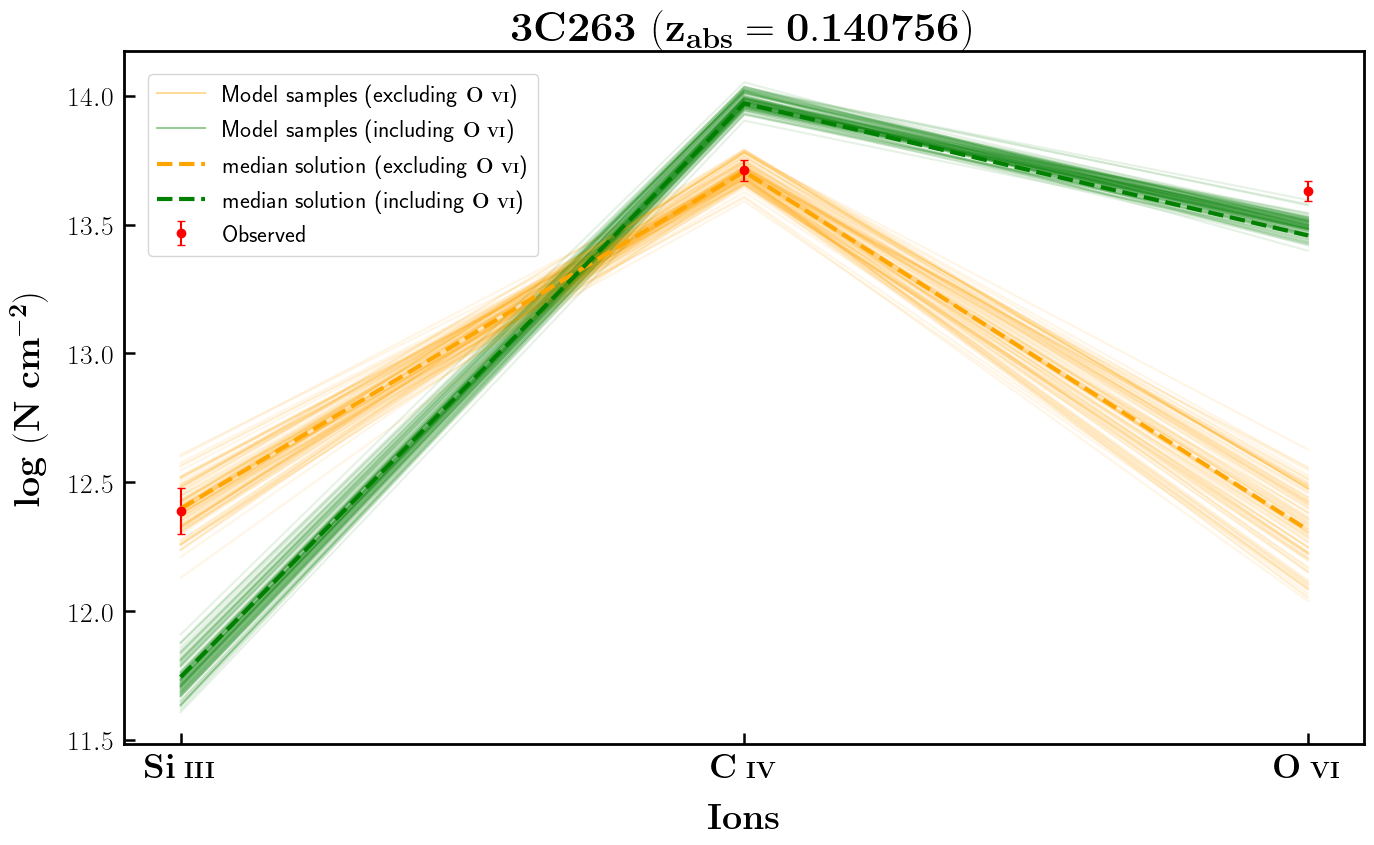
\includegraphics[width=0.9\linewidth]{Ionisation-Modelling-Plots/3c263-z=0.140756-compI_logZ=1.png}
      \caption{$\log \text{N}(\ion{H}{i}) \ [\text{cm}^{-2}]=$ 13.49}
  \end{figure}
  
    
  
  \newpage
  \thispagestyle{empty}
  
  \begin{landscape}
  
      \begin{figure}
      \centering
      \vspace{-10mm}
      \hspace*{-20mm}
      \captionsetup{oneside,margin={0cm,20mm}}
      \includegraphics[width=1.1\linewidth]{System-Plots/PKS0637-752_z=0.161064_sys_plot.png}
      \caption{System plot for the absorber along the LOS of PKS 0637-752 at $z_{abs} = 0.161064$. }
      \end{figure}
      
  \end{landscape}
  
  
  \begin{center}
   
  \begin{tabular}{cccc}
          \hline \hline \tabularnewline
          \head{Ion} & \head{v (km s\textsuperscript{$\mathbf{-1}$})} & \head{b (km s\textsuperscript{$\mathbf{-1}$})} & \head{log [N cm\textsuperscript{$\mathbf{-2}$}]} 
          \tabularnewline \tabularnewline \hline \tabularnewline 
  
          \ion{N}{v}   &    -42 $\pm$ 6    &    40 $\pm$ 9    &     13.37 $\pm$ 0.07 \\
          \ion{Si}{iii}   &    11 $\pm$ 4    &    30 $\pm$ 7    &     12.37 $\pm$ 0.06 \\
          \ion{O}{vi}   &    0 $\pm$ 3    &    48 $\pm$ 5    &     14.02 $\pm$ 0.03 \\
          \ion{H}{i}   &    -13 $\pm$ 2    &    162 $\pm$ 21    &     13.6 $\pm$ 0.06 \\
          \ion{H}{i}   &    -1 $\pm$ 1    &    45 $\pm$ 1    &     15.01 $\pm$ 0.02 \\
  \tabularnewline \hline \hline \tabularnewline
  
  \end{tabular}
  
  \end{center}
  
  $\log \text{N}(\ion{H}{i}) \ [\text{cm}^{-2}]=$ 13.60 \\
  
  Excluding \ion{O}{vi} : $\log n_H \ (\text{cm}^{-3})$ = -4.29 $\pm$ 0.02 \hspace{10mm} $\log \ Z/Z_\odot$ = 1.64 $\pm$ 0.05
  
  Including \ion{O}{vi} : $\log n_H \ (\text{cm}^{-3})$ = -4.42 $\pm$ 0.01 \hspace{10mm} $\log \ Z/Z_\odot$ = 1.69 $\pm$ 0.04 \\
  
  
  \begin{figure}[!h]
    \centering
    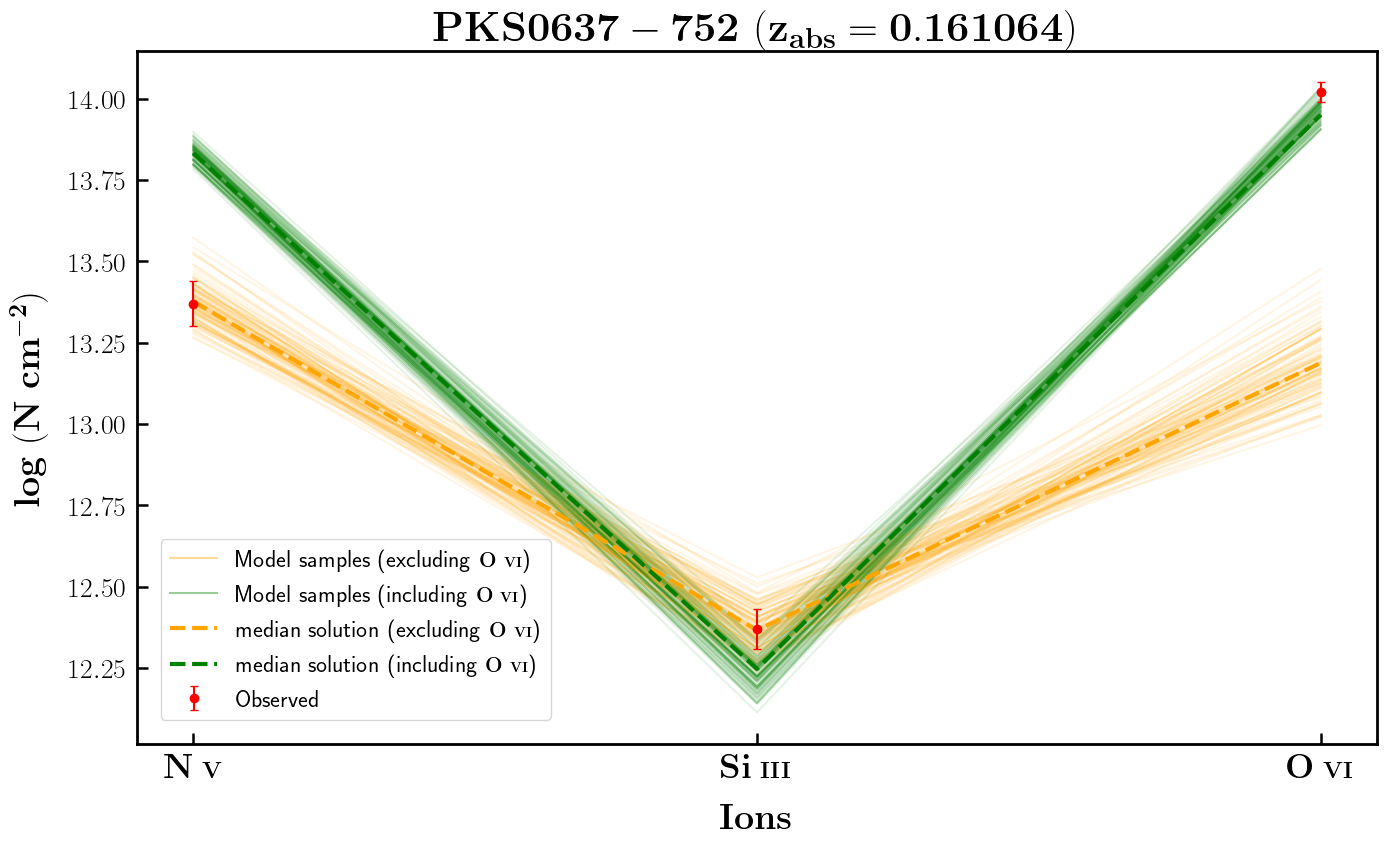
\includegraphics[width=0.9\linewidth]{Ionisation-Modelling-Plots/pks0637-z=0.161064-compI_logZ=1.png}
    \caption{$\log \text{N}(\ion{H}{i}) \ [\text{cm}^{-2}]=$ 13.60}
  \end{figure}
  
  
  
  \newpage
  \thispagestyle{empty}
  
  \begin{landscape}
  
      \begin{figure}
      \centering
      \vspace{-10mm}
      \hspace*{-20mm}
      \captionsetup{oneside,margin={0cm,20mm}}
      \includegraphics[width=1.1\linewidth]{System-Plots/PKS0637-752_z=0.417539_sys_plot.png}
      \caption{System plot for the absorber along the LOS of PKS 0637-752 at $z_{abs} = 0.417539$. }
      \end{figure}
      
  \end{landscape}
  
  
  \begin{center}
      
      \begin{tabular}{cccc}
          \hline \hline \tabularnewline
          \head{Ion} & \head{v (km s\textsuperscript{$\mathbf{-1}$})} & \head{b (km s\textsuperscript{$\mathbf{-1}$})} & \head{log [N cm\textsuperscript{$\mathbf{-2}$}]} 
          \tabularnewline \tabularnewline \hline \tabularnewline 
      
          \ion{Si}{iii}   &    -5 $\pm$ 4    &    35 $\pm$ 7    &     12.74 $\pm$ 0.06 \\
          \ion{C}{iii}   &    -4 $\pm$ 1    &    24 $\pm$ 2    &     14.44 $\pm$ 0.15 \\
          \ion{O}{vi}   &    0 $\pm$ 1    &    42 $\pm$ 6    &     14.19 $\pm$ 0.05 \\
          \ion{H}{i}   &    -17 $\pm$ 1    &    30 $\pm$ 1    &     15.41 $\pm$ 0.03 \\
          \ion{H}{i}   &    20 $\pm$ 1    &    46 $\pm$ 4    &     14.61 $\pm$ 0.07 \\
          
          \tabularnewline \hline \hline \tabularnewline
      
      \end{tabular}
      
  \end{center}
      
  $\log \text{N}(\ion{H}{i}) \ [\text{cm}^{-2}]=$ 15.41 \\
  
  Excluding \ion{O}{vi} : $\log n_H \ (\text{cm}^{-3})$ = -3.54 $\pm$ 0.11 \hspace{10mm} $\log \ Z/Z_\odot$ = -0.49 $\pm$ 0.11
  
  Including \ion{O}{vi} : $\log n_H \ (\text{cm}^{-3})$ = -3.74 $\pm$ 0.02 \hspace{10mm} $\log \ Z/Z_\odot$ = -0.23 $\pm$ 0.04 \\
  
  
  \begin{figure}[!h]
    \centering
    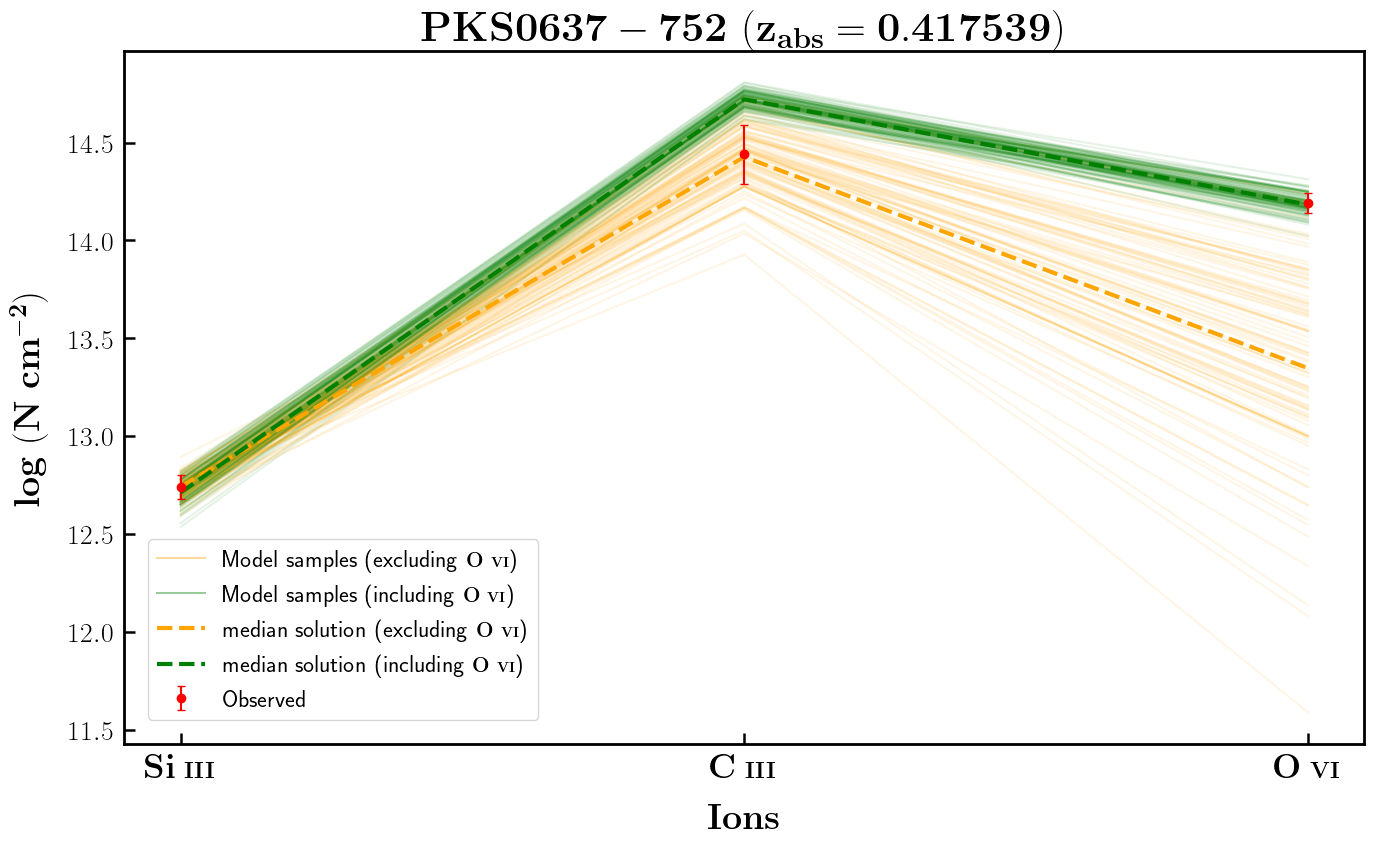
\includegraphics[width=0.9\linewidth]{Ionisation-Modelling-Plots/pks0637-z=0.417539-compI.png}
    \caption{$\log \text{N}(\ion{H}{i}) \ [\text{cm}^{-2}]=$ 15.41}
  \end{figure}
  
  
  \newpage
  \thispagestyle{empty}
  
  \begin{landscape}
  
      \begin{figure}
      \centering
      \vspace{-10mm}
      \hspace*{-20mm}
      \captionsetup{oneside,margin={0cm,20mm}}
      \includegraphics[width=1.1\linewidth]{System-Plots/PG1424+240_z=0.147104_sys_plot.png}
      \caption{System plot for the absorber along the LOS of PG 1424+240 at $z_{abs} = 0.147104$. }
      \end{figure}
      
  \end{landscape}
  
  
  \begin{center}
      
      \begin{tabular}{cccc}
              \hline \hline \tabularnewline
              \head{Ion} & \head{v (km s\textsuperscript{$\mathbf{-1}$})} & \head{b (km s\textsuperscript{$\mathbf{-1}$})} & \head{log [N cm\textsuperscript{$\mathbf{-2}$}]} 
              \tabularnewline \tabularnewline \hline \tabularnewline 
      
              \ion{C}{iv}   &    -81 $\pm$ 2    &    11 $\pm$ 4    &     13.58 $\pm$ 0.09 \\
              \ion{C}{iv}   &    -18 $\pm$ 2    &    20 $\pm$ 3    &     14.06 $\pm$ 0.05 \\ \tabularnewline
              \ion{Si}{iii}   &    -78 $\pm$ 2    &    15 $\pm$ 3    &     12.58 $\pm$ 0.05 \\
              \ion{Si}{iii}   &    -9 $\pm$ 1    &    16 $\pm$ 2    &     12.87 $\pm$ 0.03 \\ \tabularnewline
              \ion{Si}{iv}   &    -82 $\pm$ 4    &    13 $\pm$ 7    &     12.69 $\pm$ 0.1 \\
              \ion{Si}{iv}   &    -11 $\pm$ 2    &    11 $\pm$ 5    &     12.88 $\pm$ 0.07 \\ \tabularnewline
              \ion{O}{vi}   &    -56 $\pm$ 9    &    39 $\pm$ 13    &     13.77 $\pm$ 0.11 \\
              \ion{O}{vi}   &    4 $\pm$ 4    &    16 $\pm$ 6    &     13.73 $\pm$ 0.11 \\ \tabularnewline
              \ion{H}{i}   &    -454 $\pm$ 3    &    27 $\pm$ 5    &     13.16 $\pm$ 0.05 \\
              \ion{H}{i}   &    -87 $\pm$ 3    &    23 $\pm$ 2    &     14.88 $\pm$ 0.05 \\
              \ion{H}{i}   &    0 $\pm$ 3    &    29 $\pm$ 2    &     15.44 $\pm$ 0.14 \\
              \ion{H}{i}   &    216 $\pm$ 2    &    40 $\pm$ 3    &     13.49 $\pm$ 0.02 \\
              \tabularnewline \hline \hline \tabularnewline
      
      \end{tabular}
  
  \end{center}
  
  $\log \text{N}(\ion{H}{i}) \ [\text{cm}^{-2}]=$ 15.44 \\
  
  Excluding \ion{O}{vi} : $\log n_H \ (\text{cm}^{-3})$ = -3.81 $\pm$ 0.03 \hspace{10mm} $\log \ Z/Z_\odot$ = -0.46 $\pm$ 0.03
  
  Including \ion{O}{vi} : $\log n_H \ (\text{cm}^{-3})$ = -3.88 $\pm$ 0.02 \hspace{10mm} $\log \ Z/Z_\odot$ = -0.42 $\pm$ 0.02 \\
  
  $\log \text{N}(\ion{H}{i}) \ [\text{cm}^{-2}]=$ 14.88 \\
  
  Excluding \ion{O}{vi} : $\log n_H \ (\text{cm}^{-3})$ = -3.74 $\pm$ 0.05 \hspace{10mm} $\log \ Z/Z_\odot$ = -0.22 $\pm$ 0.04
  
  Including \ion{O}{vi} : $\log n_H \ (\text{cm}^{-3})$ = -3.96 $\pm$ 0.03 \hspace{10mm} $\log \ Z/Z_\odot$ = -0.07 $\pm$ 0.04
  
  \newpage
  
  \begin{figure}[!h]
    \centering
      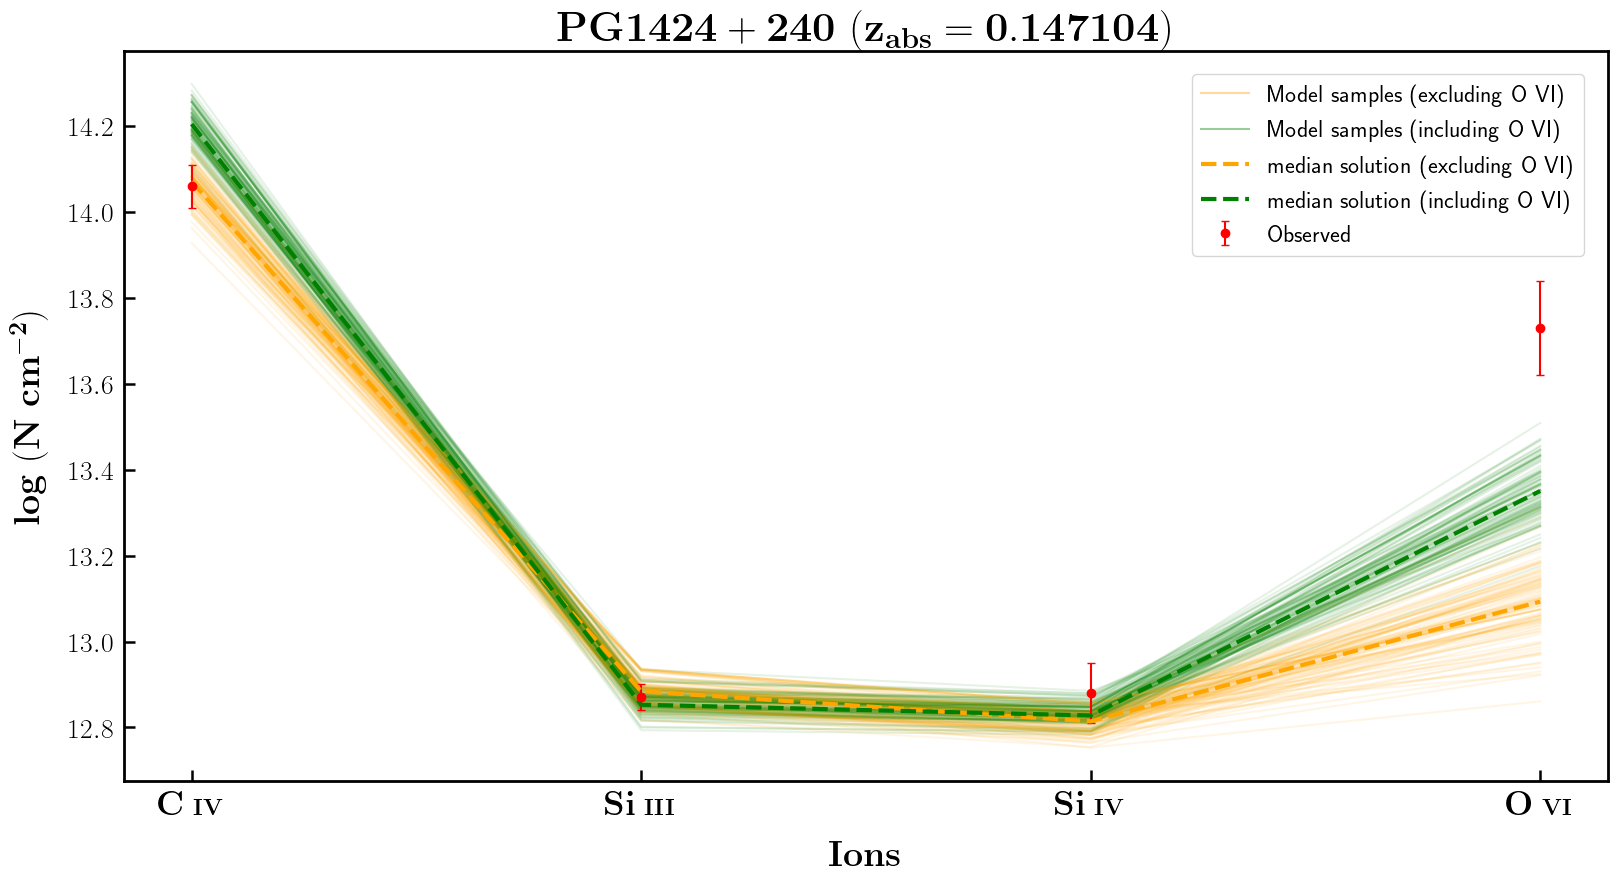
\includegraphics[width=0.9\linewidth]{Ionisation-Modelling-Plots/pg1424-z=0.147104-compIII.png}
      \caption{$\log \text{N}(\ion{H}{i}) \ [\text{cm}^{-2}]=$ 15.44}
  \end{figure}
  
  \begin{figure}[!b]
    \centering
      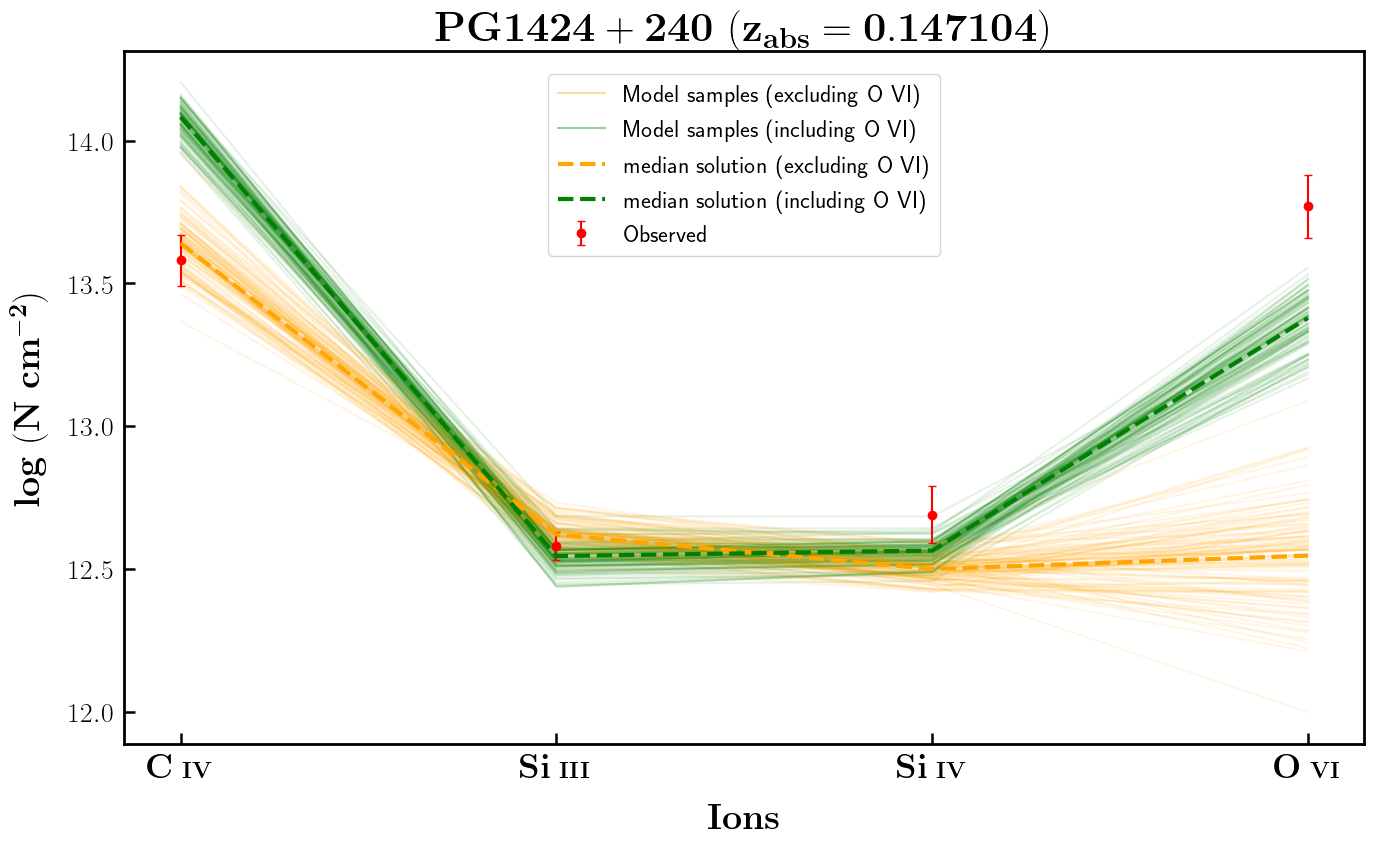
\includegraphics[width=0.9\linewidth]{Ionisation-Modelling-Plots/pg1424-z=0.147104-compII.png}
      \caption{$\log \text{N}(\ion{H}{i}) \ [\text{cm}^{-2}]=$ 14.88}
  \end{figure}
  
  
  \newpage
  \thispagestyle{empty}
  
  \begin{landscape}
  
      \begin{figure}
      \centering
      \vspace{-10mm}
      \hspace*{-20mm}
      \captionsetup{oneside,margin={0cm,20mm}}
      \includegraphics[width=1.1\linewidth]{System-Plots/PG0003+158_z=0.386089_sys_plot.png}
      \caption{System plot for the absorber along the LOS of PG 0003+158 at $z_{abs} = 0.386089$. }
      \end{figure}
      
  \end{landscape}
  
  \newgeometry{bottom=0.1cm}
  
  \begin{center}
      
      \begin{tabular}{cccc}
          \hline \hline \tabularnewline
          \head{Ion} & \head{v (km s\textsuperscript{$\mathbf{-1}$})} & \head{b (km s\textsuperscript{$\mathbf{-1}$})} & \head{log [N cm\textsuperscript{$\mathbf{-2}$}]} 
          \tabularnewline \tabularnewline \hline \tabularnewline 
      
          \ion{O}{iii}   &    -18 $\pm$ 2    &    9 $\pm$ 5    &     13.93 $\pm$ 0.08 \\
          \ion{C}{iii}   &    -11 $\pm$ 1    &    13 $\pm$ 2    &     13.35 $\pm$ 0.05 \\
          \ion{N}{v}   &    -7 $\pm$ 1    &    33 $\pm$ 11    &     13.49 $\pm$ 0.11 \\
          \ion{O}{vi}   &    0 $\pm$ 2    &    25 $\pm$ 3    &     13.87 $\pm$ 0.04 \\
          \ion{O}{vi}   &    54 $\pm$ 3    &    25 $\pm$ 4    &     13.71 $\pm$ 0.06 \\
          \ion{H}{i}   &    -10 $\pm$ 1    &    29 $\pm$ 0    &     14.81 $\pm$ 0.03 \\
          \ion{H}{i}   &    40 $\pm$ 9    &    40 $\pm$ 4    &     14.1 $\pm$ 0.05 \\
  
          \tabularnewline \hline \hline \tabularnewline
      
      \end{tabular}
      
  \end{center}
      
  $\log \text{N}(\ion{H}{i}) \ [\text{cm}^{-2}]=$ 14.81 \\
  
  Excluding \ion{O}{vi} : $\log n_H \ (\text{cm}^{-3})$ = -4.12 $\pm$ 0.06 \hspace{10mm} $\log \ Z/Z_\odot$ = -0.65 $\pm$ 0.04
  
  Including \ion{O}{vi} : $\log n_H \ (\text{cm}^{-3})$ = -4.07 $\pm$ 0.02 \hspace{10mm} $\log \ Z/Z_\odot$ = -0.68 $\pm$ 0.03 \\
  
  \begin{figure}[!h]
    \centering
    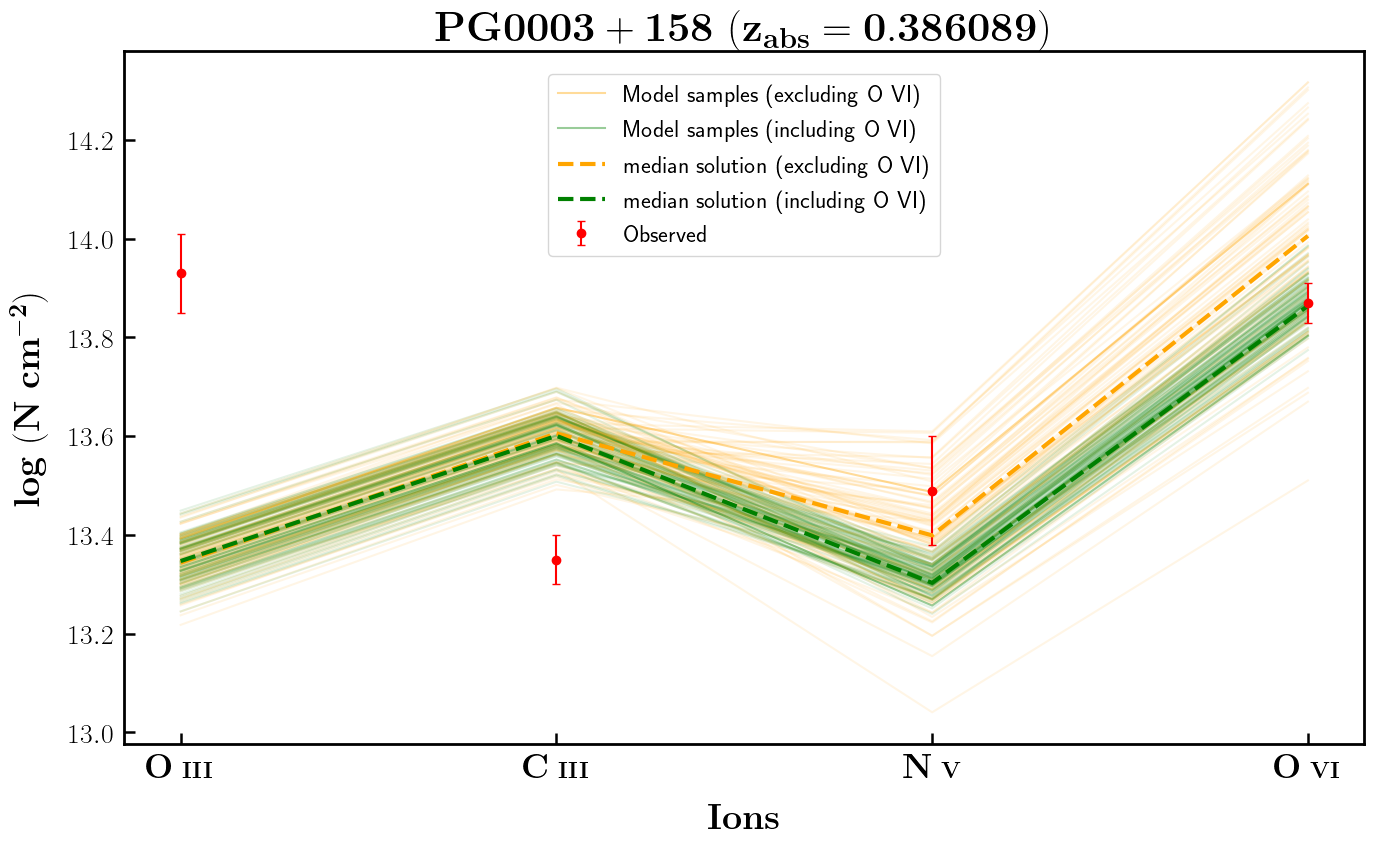
\includegraphics[width=0.9\linewidth]{Ionisation-Modelling-Plots/pg0003-z=0.386089-compI.png}
      \caption{$\log \text{N}(\ion{H}{i}) \ [\text{cm}^{-2}]=$ 14.81}
  \end{figure}
  
  \restoregeometry
  
  \newpage
  \thispagestyle{empty}
  
  \begin{landscape}
  
      \begin{figure}
      \centering
      \vspace{-10mm}
      \hspace*{-20mm}
      \captionsetup{oneside,margin={0cm,20mm}}
      \includegraphics[width=1.1\linewidth]{System-Plots/PG0003+158_z=0.421923_sys_plot.png}
      \caption{System plot for the absorber along the LOS of PG 0003+158 at $z_{abs} = 0.421923$. }
      \end{figure}
      
  \end{landscape}
  
  \newgeometry{bottom=0.1cm}
  
  \begin{center}
      
      \begin{tabular}{cccc}
          \hline \hline \tabularnewline
          \head{Ion} & \head{v (km s\textsuperscript{$\mathbf{-1}$})} & \head{b (km s\textsuperscript{$\mathbf{-1}$})} & \head{log [N cm\textsuperscript{$\mathbf{-2}$}]} 
          \tabularnewline \tabularnewline \hline \tabularnewline 
      
          \ion{C}{iii}   &    -9 $\pm$ 1    &    13 $\pm$ 1    &     13.35 $\pm$ 0.04 \\
          \ion{O}{iii}   &    -1 $\pm$ 2    &    7 $\pm$ 5    &     13.83 $\pm$ 0.13 \\
          \ion{O}{vi}   &    0 $\pm$ 1    &    27 $\pm$ 1    &     14.27 $\pm$ 0.02 \\
          \ion{H}{i}   &    -272 $\pm$ 6    &    66 $\pm$ 10    &     13.37 $\pm$ 0.05 \\
          \ion{H}{i}   &    -16 $\pm$ 1    &    64 $\pm$ 3    &     14.17 $\pm$ 0.04 \\
          \ion{H}{i}   &    -2 $\pm$ 1    &    26 $\pm$ 1    &     14.71 $\pm$ 0.02 \\
      
          \tabularnewline \hline \hline \tabularnewline
      
      \end{tabular}
      
  \end{center}
      
  $\log \text{N}(\ion{H}{i}) \ [\text{cm}^{-2}]=$ 14.17 \\
  
  Excluding \ion{O}{vi} : $\log n_H \ (\text{cm}^{-3})$ = -2.66 $\pm$ 0.22 \hspace{10mm} $\log \ Z/Z_\odot$ = 0.42 $\pm$ 0.23
  
  Including \ion{O}{vi} : $\log n_H \ (\text{cm}^{-3})$ = -4.24 $\pm$ 0.02 \hspace{10mm} $\log \ Z/Z_\odot$ = -0.09 $\pm$ 0.03 \\
  
  \begin{figure}[!h]
    \centering
    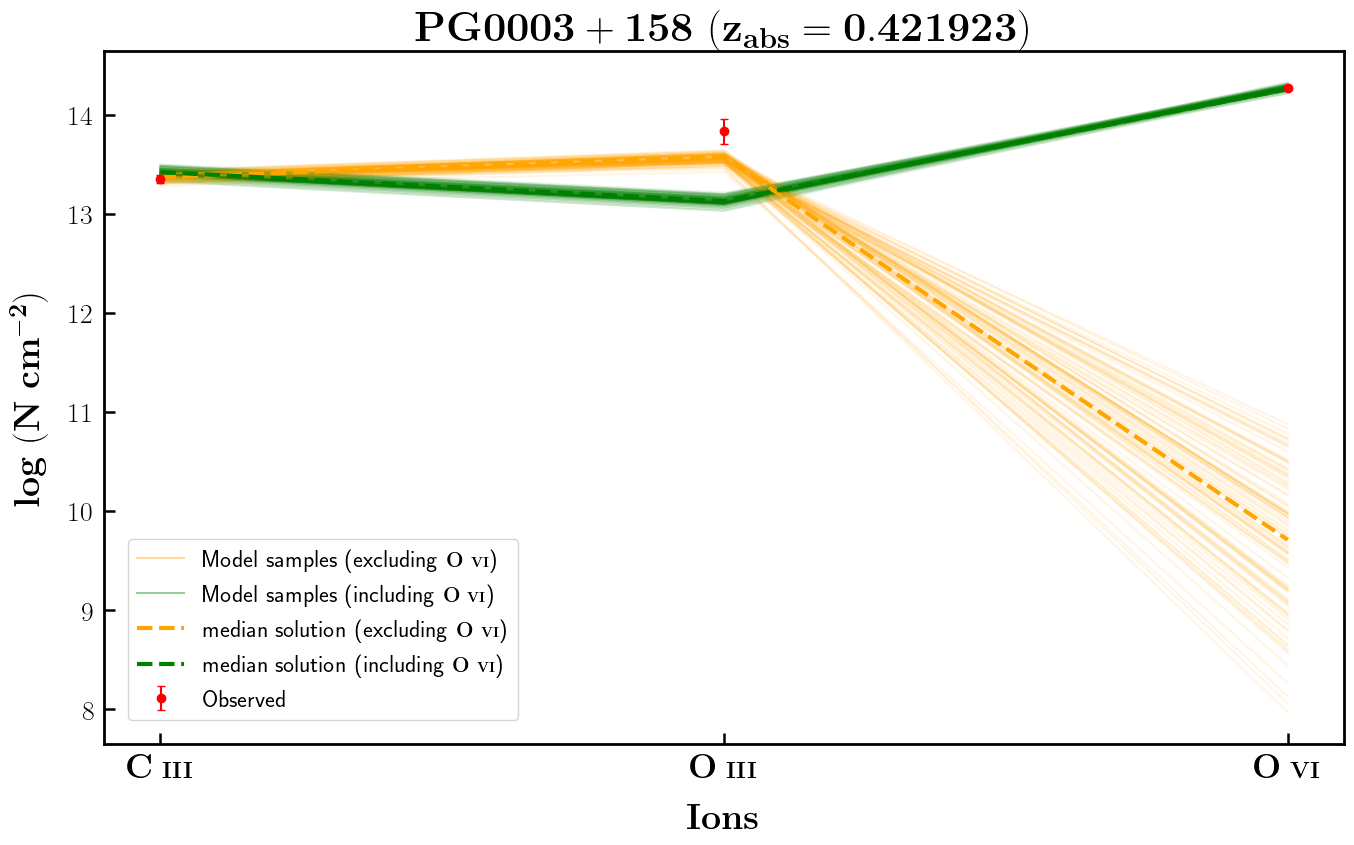
\includegraphics[width=0.9\linewidth]{Ionisation-Modelling-Plots/pg0003-z=0.421923-compII.png}
      \caption{$\log \text{N}(\ion{H}{i}) \ [\text{cm}^{-2}]=$ 14.17}
  \end{figure}

  \restoregeometry
  
  
  \newpage
  \thispagestyle{empty}
  
  \begin{landscape}
  
      \begin{figure}
      \centering
      \vspace{-10mm}
      \hspace*{-20mm}
      \captionsetup{oneside,margin={0cm,20mm}}
      \includegraphics[width=1.1\linewidth]{System-Plots/PG1216+069_z=0.282286_sys_plot.png}
      \caption{System plot for the absorber along the LOS of PG 1216+069 at $z_{abs} = 0.282286$. }
      \end{figure}
      
  \end{landscape}
  
  
  \begin{center}
   
  \begin{tabular}{cccc}
          \hline \hline \tabularnewline
          \head{Ion} & \head{v (km s\textsuperscript{$\mathbf{-1}$})} & \head{b (km s\textsuperscript{$\mathbf{-1}$})} & \head{log [N cm\textsuperscript{$\mathbf{-2}$}]} 
          \tabularnewline \tabularnewline \hline \tabularnewline 
  
          \ion{Si}{iii}   &    0 $\pm$ 1    &    14 $\pm$ 3    &     12.92 $\pm$ 0.05 \\
          \ion{C}{iii}   &    -51 $\pm$ 3    &    32 $\pm$ 5    &     13.33 $\pm$ 0.05 \\
          \ion{C}{iii}   &    5 $\pm$ 1    &    16 $\pm$ 2    &     13.76 $\pm$ 0.07 \\
          \ion{O}{vi}   &    -64 $\pm$ 6    &    58 $\pm$ 9    &     13.93 $\pm$ 0.05 \\
          \ion{O}{vi}   &    19 $\pm$ 2    &    12 $\pm$ 5    &     13.54 $\pm$ 0.09 \\
          \ion{H}{i}   &    -31 $\pm$ 1    &    52 $\pm$ 3    &     15.1 $\pm$ 0.05 \\
          \ion{H}{i}   &    7 $\pm$ 1    &    22 $\pm$ 1    &     16.4 $\pm$ 0.03 \\
          \ion{H}{i}   &    169 $\pm$ 22    &    53 $\pm$ 10    &     13.15 $\pm$ 0.18 \\
  
          \tabularnewline \hline \hline \tabularnewline
  
  \end{tabular}
      
  \end{center}
      
  $\log \text{N}(\ion{H}{i}) \ [\text{cm}^{-2}]=$ 15.10 \\
  
  Excluding \ion{O}{vi} : $\log n_H \ (\text{cm}^{-3})$ = -2.13 $\pm$ 0.15 \hspace{10mm} $\log \ Z/Z_\odot$ = 0.65 $\pm$ 0.22
  
  Including \ion{O}{vi} : $\log n_H \ (\text{cm}^{-3})$ = -3.86 $\pm$ 0.02 \hspace{10mm} $\log \ Z/Z_\odot$ = -0.37 $\pm$ 0.03 \\
  
  $\log \text{N}(\ion{H}{i}) \ [\text{cm}^{-2}]=$ 16.40 \\
  
  Excluding \ion{O}{vi} : $\log n_H \ (\text{cm}^{-3})$ = -2.08 $\pm$ 0.43 \hspace{10mm} $\log \ Z/Z_\odot$ = -0.37 $\pm$ 0.59
  
  Including \ion{O}{vi} : $\log n_H \ (\text{cm}^{-3})$ = -3.68 $\pm$ 0.02 \hspace{10mm} $\log \ Z/Z_\odot$ = -1.55 $\pm$ 0.04 
  \newpage
  
  
  \begin{figure}[!h]
      \centering
      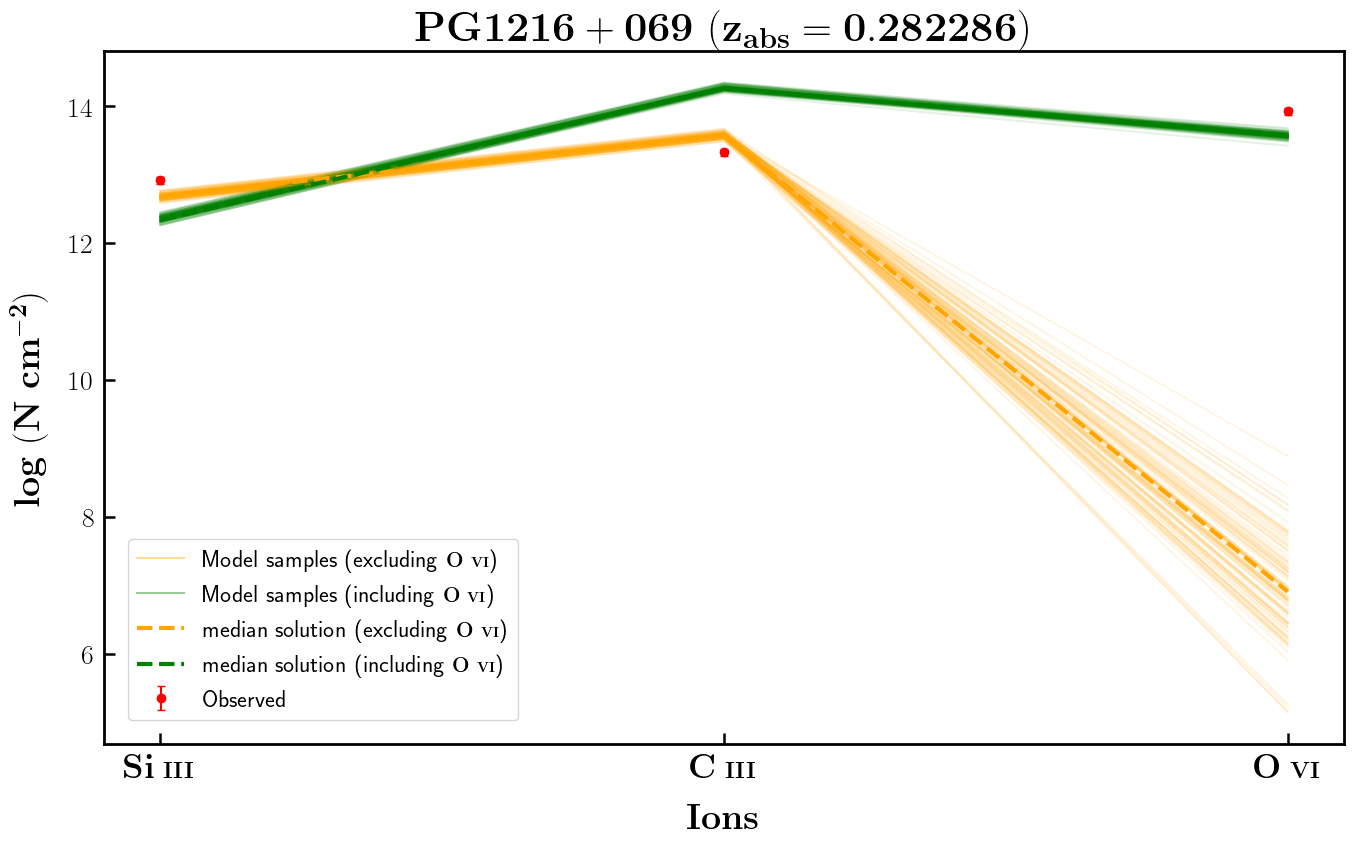
\includegraphics[width=0.9\linewidth]{Ionisation-Modelling-Plots/pg1216-z=0.282286-compI.png}
      \caption{$\log \text{N}(\ion{H}{i}) \ [\text{cm}^{-2}]=$ 15.10}
  \end{figure}
  
  \begin{figure}[!b]
      \centering
      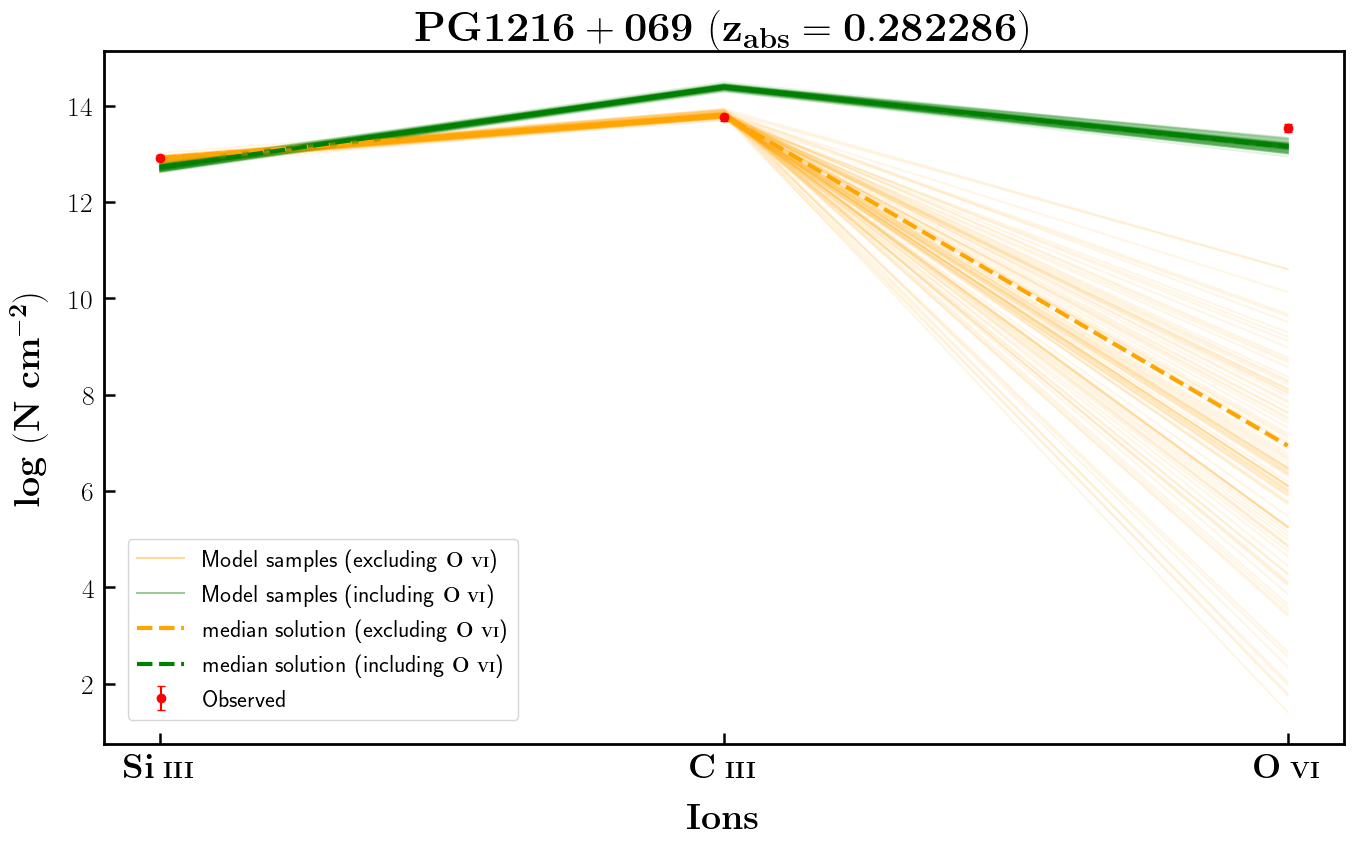
\includegraphics[width=0.9\linewidth]{Ionisation-Modelling-Plots/pg1216-z=0.282286-compII.png}
      \caption{$\log \text{N}(\ion{H}{i}) \ [\text{cm}^{-2}]=$ 16.40}
  \end{figure}
  
  
  \newpage
  \thispagestyle{empty}
  
  \begin{landscape}
  
  \begin{figure}
      \centering
      \vspace{-10mm}
      \hspace*{-20mm}
      \captionsetup{oneside,margin={0cm,20mm}}
      \includegraphics[width=1.1\linewidth]{System-Plots/SDSSJ135712.61+170444_z=0.097869_sys_plot.png}
      \caption{System plot for the absorber along the LOS of SDSS J135712.61+170444 at $z_{abs} = 0.097869$. }
  \end{figure}
  
  \end{landscape}
  
  \newgeometry{top=22mm,bottom=0.1cm}
  
  \begin{center} 
  
  \begin{tabular}{cccc} 
  
      \hline \hline \tabularnewline 
      \head{Ion} & \head{v (km s\textsuperscript{$\mathbf{-1}$})} & \head{b (km s\textsuperscript{$\mathbf{-1}$})} & \head{log [N cm\textsuperscript{$\mathbf{-2}$}]}
      \tabularnewline \tabularnewline \hline \tabularnewline 
   
      \ion{Si}{iii}   &    -62 $\pm$ 2    &    17 $\pm$ 3    &     12.94 $\pm$ 0.05 \\
      \ion{Si}{iii}   &    4 $\pm$ 1    &    13 $\pm$ 10    &     14.67 $\pm$ 2.87 \\
      \ion{C}{iv}   &    -74 $\pm$ 6    &    33 $\pm$ 1    &     13.82 $\pm$ 0.09 \\
      \ion{C}{iv}   &    -7 $\pm$ 8    &    32 $\pm$ 12    &     13.63 $\pm$ 0.12 \\
      \ion{Si}{iv}   &    -66 $\pm$ 4    &    18 $\pm$ 6    &     13.02 $\pm$ 0.08 \\
      \ion{Si}{iv}   &    0 $\pm$ 4    &    29 $\pm$ 5    &     13.3 $\pm$ 0.05 \\
      \ion{C}{ii}   &    -79 $\pm$ 8    &    19 $\pm$ 14    &     13.17 $\pm$ 0.16 \\
      \ion{C}{ii}   &    -1 $\pm$ 2    &    22 $\pm$ 3    &     13.92 $\pm$ 0.04 \\
      \ion{O}{vi}   &    -96 $\pm$ 10    &    43 $\pm$ 16    &     14.3 $\pm$ 0.11 \\
      \ion{H}{i}   &    -536 $\pm$ 3    &    29 $\pm$ 5    &     13.36 $\pm$ 0.05 \\
      \ion{H}{i}   &    -66 $\pm$ 0    &    29 $\pm$ 8    &     16.49 $\pm$ 0.12 \\
      \ion{H}{i}   &    0 $\pm$ 0    &    46 $\pm$ 4    &     15.01 $\pm$ 0.16 \\
      \ion{H}{i}   &    424 $\pm$ 3    &    34 $\pm$ 4    &     13.52 $\pm$ 0.04 \\
  
      \tabularnewline \hline \hline \tabularnewline 
  
  \end{tabular}
  
  \end{center}
  
  
  $\log \text{N}(\ion{H}{i}) \ [\text{cm}^{-2}]=$ 16.49 \\
  
  Excluding \ion{O}{vi} : $\log n_H \ (\text{cm}^{-3})$ = -3.76 $\pm$ 0.05 \hspace{10mm} $\log \ Z/Z_\odot$ = -1.49 $\pm$ 0.04
  
  Including \ion{O}{vi} : $\log n_H \ (\text{cm}^{-3})$ = -4.06 $\pm$ 0.02 \hspace{10mm} $\log \ Z/Z_\odot$ = -1.32 $\pm$ 0.04 \\
  
  \begin{figure}[!h]
      \centering
      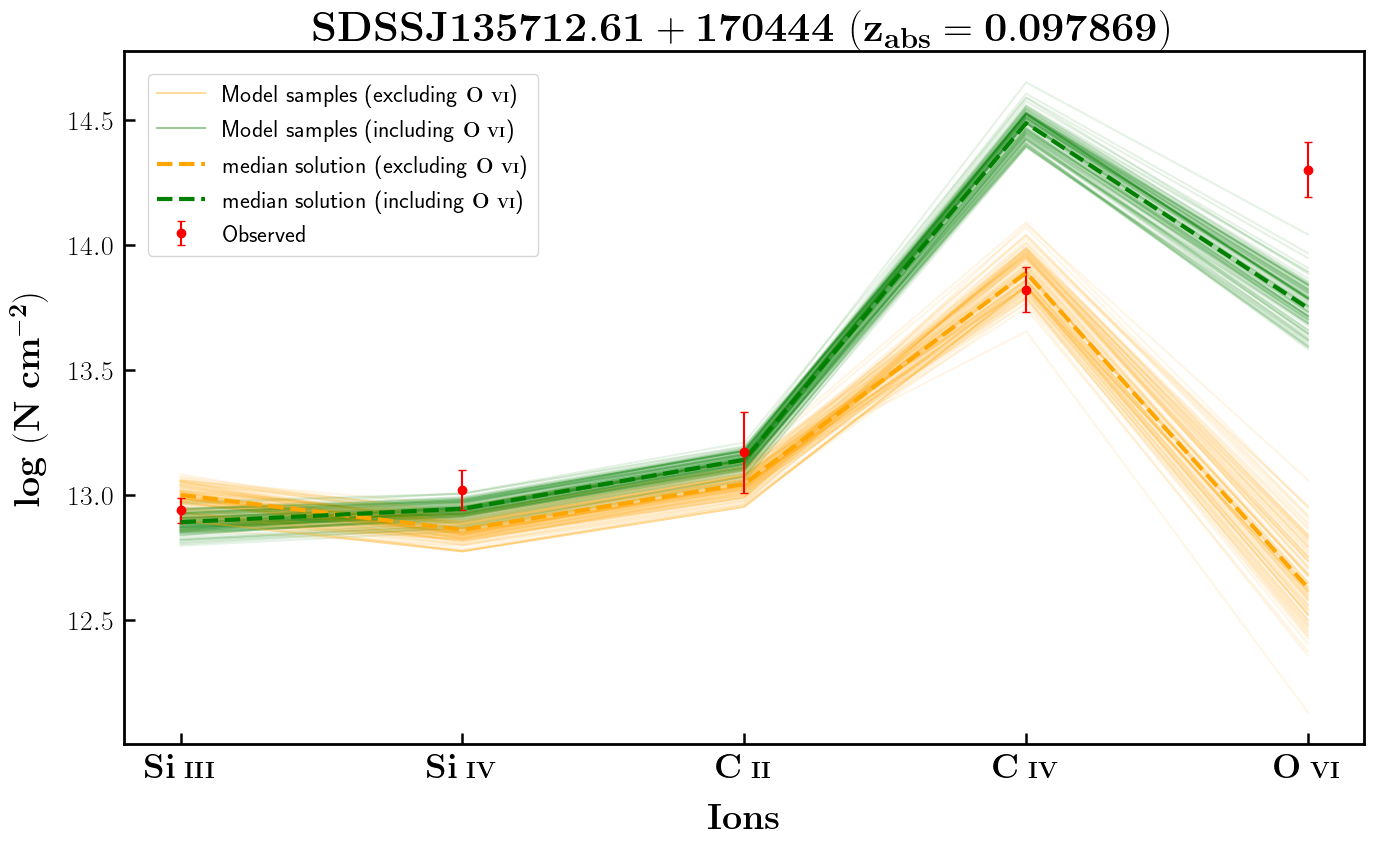
\includegraphics[width=0.9\linewidth]{Ionisation-Modelling-Plots/s135712-z=0.097869-compII.png}
      \caption{$\log \text{N}(\ion{H}{i}) \ [\text{cm}^{-2}]=$ 16.49}
  \end{figure}
  
  \restoregeometry
  
  \newpage
  \thispagestyle{empty}

  \begin{landscape}
  
  \begin{figure}
      \centering
      \vspace{-10mm}
      \hspace*{-20mm}
      \captionsetup{oneside,margin={0cm,20mm}}
      \includegraphics[width=1.1\linewidth]{System-Plots/1ES1553+113_z=0.187764_sys_plot.png}
      \caption{System plot for the absorber along the LOS of 1ES 1553+113 at $z_{abs} = 0.187764$. }
  \end{figure}
  
  \end{landscape}
  
  
  \begin{center} 
  
  \begin{tabular}{cccc} 
  
      \hline \hline \tabularnewline 
      \head{Ion} & \head{v (km s\textsuperscript{$\mathbf{-1}$})} & \head{b (km s\textsuperscript{$\mathbf{-1}$})} & \head{log [N cm\textsuperscript{$\mathbf{-2}$}]}
      \tabularnewline \tabularnewline \hline \tabularnewline 
   
      \ion{C}{iii}   &    -46 $\pm$ 1    &    5 $\pm$ 4    &     13.17 $\pm$ 0.46 \\
      \ion{C}{iii}   &    -6 $\pm$ 1    &    13 $\pm$ 2    &     13.21 $\pm$ 0.03 \\
      \ion{N}{v}   &    -47 $\pm$ 2    &    17 $\pm$ 0    &     13.43 $\pm$ 0.05 \\
      \ion{N}{v}   &    -5 $\pm$ 2    &    16 $\pm$ 4    &     13.33 $\pm$ 0.06 \\
      \ion{O}{vi}   &    -42 $\pm$ 1    &    3 $\pm$ 1    &     14.23 $\pm$ 0.33 \\
      \ion{O}{vi}   &    0 $\pm$ 1    &    15 $\pm$ 3    &     13.71 $\pm$ 0.03 \\
      \ion{O}{vi}   &    511 $\pm$ 3    &    28 $\pm$ 5    &     13.49 $\pm$ 0.05 \\
      \ion{H}{i}   &    -52 $\pm$ 3    &    8 $\pm$ 6    &     12.76 $\pm$ 0.15 \\
      \ion{H}{i}   &    -28 $\pm$ 1    &    51 $\pm$ 1    &     13.88 $\pm$ 0.01 \\
      \ion{H}{i}   &    425 $\pm$ 3    &    25 $\pm$ 5    &     13.02 $\pm$ 0.07 \\
      \ion{H}{i}   &    496 $\pm$ 2    &    37 $\pm$ 3    &     13.46 $\pm$ 0.03 \\
  
      \tabularnewline \hline \hline \tabularnewline 
  
  \end{tabular}
  
  \end{center}
  
  $\log \text{N}(\ion{H}{i}) \ [\text{cm}^{-2}]=$ 12.76 \\
  
  Excluding \ion{O}{vi} : $\log n_H \ (\text{cm}^{-3})$ = -4.62 $\pm$ 0.04 \hspace{10mm} $\log \ Z/Z_\odot$ = 1.37 $\pm$ 0.06
  
  Including \ion{O}{vi} : $\log n_H \ (\text{cm}^{-3})$ = -4.63 $\pm$ 0.03 \hspace{10mm} $\log \ Z/Z_\odot$ = 1.37 $\pm$ 0.06
  \\\\
  
  $\log \text{N}(\ion{H}{i}) \ [\text{cm}^{-2}]=$ 13.88 \\
  
  Excluding \ion{O}{vi} : $\log n_H \ (\text{cm}^{-3})$ = -4.6 $\pm$ 0.04 \hspace{10mm} $\log \ Z/Z_\odot$ = 0.03 $\pm$ 0.03
  
  Including \ion{O}{vi} : $\log n_H \ (\text{cm}^{-3})$ = -4.44 $\pm$ 0.02 \hspace{10mm} $\log \ Z/Z_\odot$ = -0.06 $\pm$ 0.02
  \\\\
  
  
  \newpage
  
  
  \begin{figure}[!h]
      \centering
      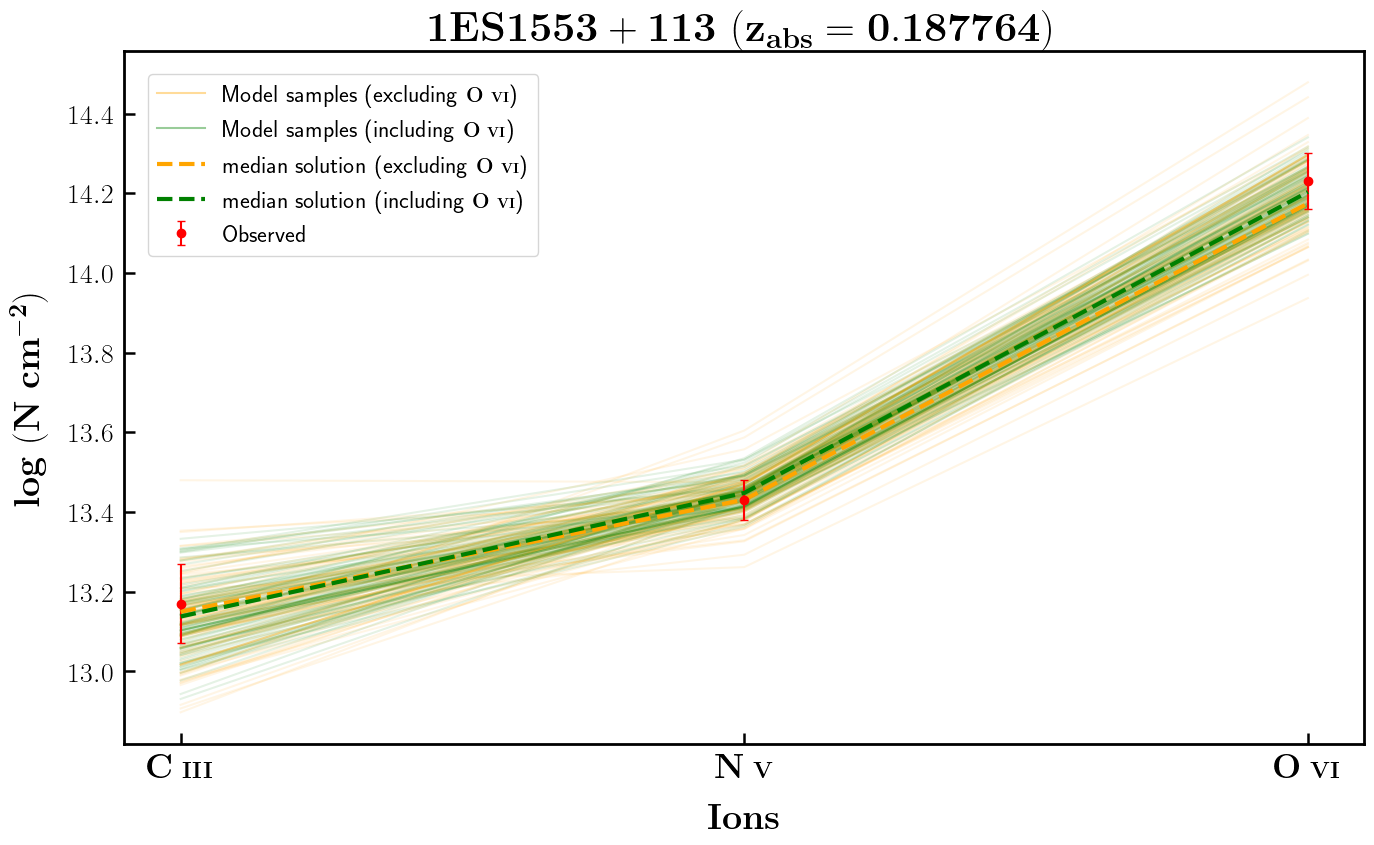
\includegraphics[width=0.9\linewidth]{Ionisation-Modelling-Plots/1es1553-z=0.187764-compI.png}
      \caption{$\log \text{N}(\ion{H}{i}) \ [\text{cm}^{-2}]=$ 12.76}
  \end{figure}
  
  \begin{figure}[!b]
      \centering
      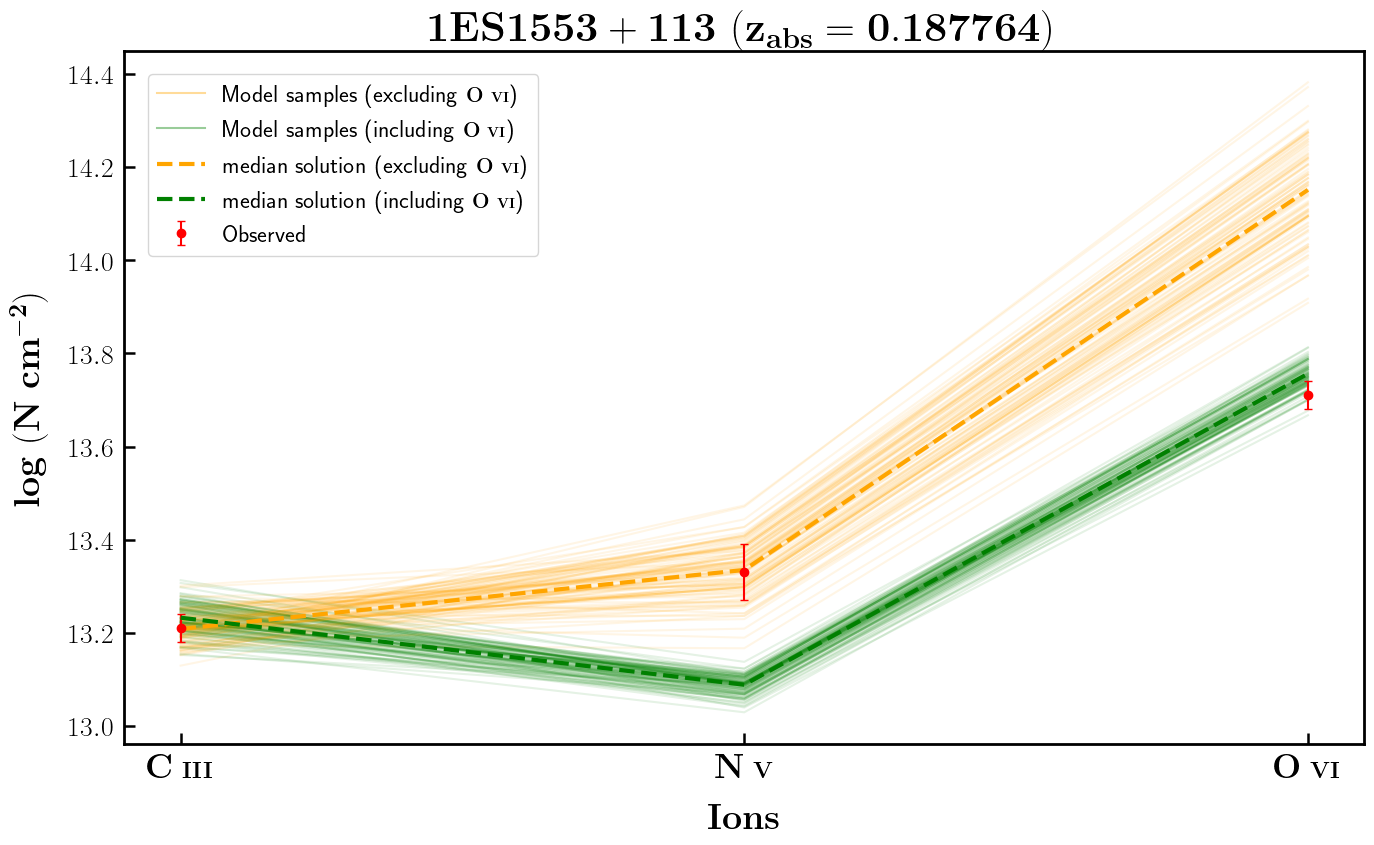
\includegraphics[width=0.9\linewidth]{Ionisation-Modelling-Plots/1es1553-z=0.187764-compII.png}
      \caption{$\log \text{N}(\ion{H}{i}) \ [\text{cm}^{-2}]=$ 13.88}
  \end{figure}
  
  
  
  \newpage
  \thispagestyle{empty}

  \begin{landscape}
  
  \begin{figure}
      \centering
      \vspace{-10mm}
      \hspace*{-20mm}
      \captionsetup{oneside,margin={0cm,20mm}}
      \includegraphics[width=1.1\linewidth]{System-Plots/SBS1108+560_z=0.463207_sys_plot.png}
      \caption{System plot for the absorber along the LOS of SBS 1108+560 at $z_{abs} = 0.463207$. }
  \end{figure}
  
  \end{landscape}
  
  
  \begin{center} 
  
  \begin{tabular}{cccc} 
  
      \hline \hline \tabularnewline 
      \head{Ion} & \head{v (km s\textsuperscript{$\mathbf{-1}$})} & \head{b (km s\textsuperscript{$\mathbf{-1}$})} & \head{log [N cm\textsuperscript{$\mathbf{-2}$}]}
      \tabularnewline \tabularnewline \hline \tabularnewline 
   
      \ion{O}{i}   &    25 $\pm$ 2    &    18 $\pm$ 4    &     14.13 $\pm$ 0.05 \\
      \ion{Si}{iii}   &    -23 $\pm$ 9    &    39 $\pm$ 12    &     13.26 $\pm$ 0.12 \\
      \ion{Si}{iii}   &    21 $\pm$ 2    &    13 $\pm$ 15    &     14.61 $\pm$ 0.24 \\
      \ion{C}{ii}   &    12 $\pm$ 9    &    31 $\pm$ 4    &     14.15 $\pm$ 0.05 \\
      \ion{C}{ii}   &    34 $\pm$ 2    &    12 $\pm$ 5    &     14.67 $\pm$ 0.1 \\
      \ion{C}{iii}   &    -48 $\pm$ 3    &    15 $\pm$ 1    &     13.66 $\pm$ 0.08 \\
      \ion{C}{iii}   &    -10 $\pm$ 3    &    26 $\pm$ 7    &     14.16 $\pm$ 0.07 \\
      \ion{C}{iii}   &    28 $\pm$ 3    &    24 $\pm$ 1    &     13.95 $\pm$ 0.05 \\
      \ion{N}{iii}   &    -22 $\pm$ 59    &    67 $\pm$ 61    &     13.77 $\pm$ 0.1 \\
      \ion{N}{iii}   &    32 $\pm$ 2    &    26 $\pm$ 4    &     14.49 $\pm$ 0.09 \\
      \ion{Si}{ii}   &    25 $\pm$ 1    &    15 $\pm$ 1    &     13.57 $\pm$ 0.08 \\
      \ion{O}{vi}   &    0 $\pm$ 6    &    45 $\pm$ 10    &     13.71 $\pm$ 0.07 \\
      \ion{H}{i}   &    -48 $\pm$ 0    &    22 $\pm$ 2    &     15.77 $\pm$ 0.02 \\
      \ion{H}{i}   &    -10 $\pm$ 2    &    16 $\pm$ 0    &     15.79 $\pm$ 0.11 \\
      \ion{H}{i}   &    28 $\pm$ 1    &    16 $\pm$ 1    &     18.1 $\pm$ 0.12 \\
      
      \tabularnewline \hline \hline \tabularnewline 
  
  \end{tabular}
  
  \end{center}
  
  
  $\log \text{N}(\ion{H}{i}) \ [\text{cm}^{-2}]=$ 18.10 \\
  
  Excluding \ion{O}{vi} : $\log n_H \ (\text{cm}^{-3})$ = -2.55 $\pm$ 0.03 \hspace{10mm} $\log \ Z/Z_\odot$ = -0.83 $\pm$ 0.04
  
  Including \ion{O}{vi} : $\log n_H \ (\text{cm}^{-3})$ = -3.49 $\pm$ 0.01 \hspace{10mm} $\log \ Z/Z_\odot$ = -0.92 $\pm$ 0.03
  \\
  
  $\log \text{N}(\ion{H}{i}) \ [\text{cm}^{-2}]=$ 15.79 \\
  
  Excluding \ion{O}{vi} : $\log n_H \ (\text{cm}^{-3})$ = -2.65 $\pm$ 0.22 \hspace{10mm} $\log \ Z/Z_\odot$ = 1.60 $\pm$ 0.22
  
  Including \ion{O}{vi} : $\log n_H \ (\text{cm}^{-3})$ = -3.56 $\pm$ 0.03 \hspace{10mm} $\log \ Z/Z_\odot$ = 1.16 $\pm$ 0.05
  
  
  \newpage
  
  \begin{figure}[!h]
    \centering
    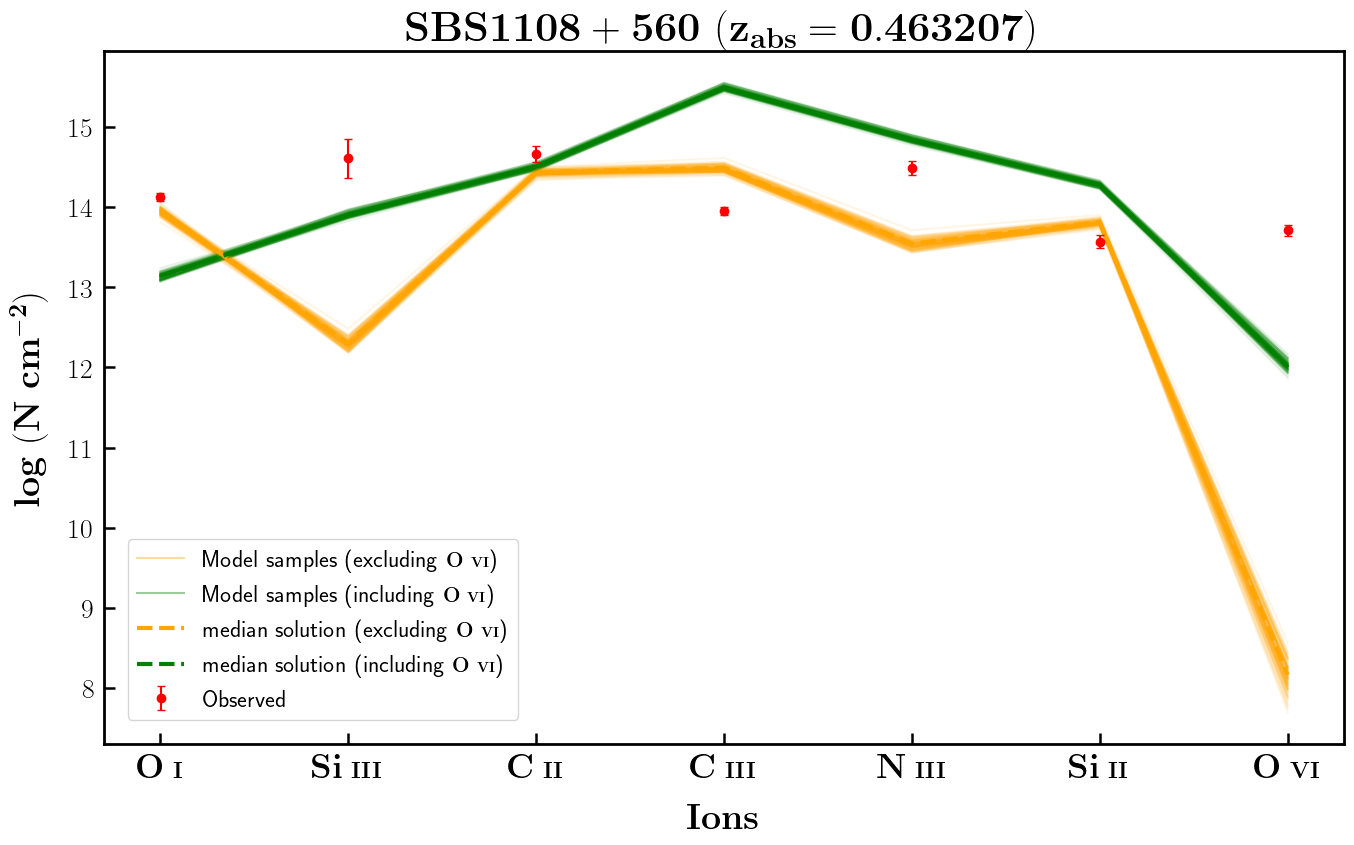
\includegraphics[width=0.9\linewidth]{Ionisation-Modelling-Plots/sbs1108-z=0.463207-compIII_logZ=1.png}
    \caption{$\log \text{N}(\ion{H}{i}) \ [\text{cm}^{-2}]=$ 18.10}
  \end{figure}
  
  
  \begin{figure}[!b]
      \centering
      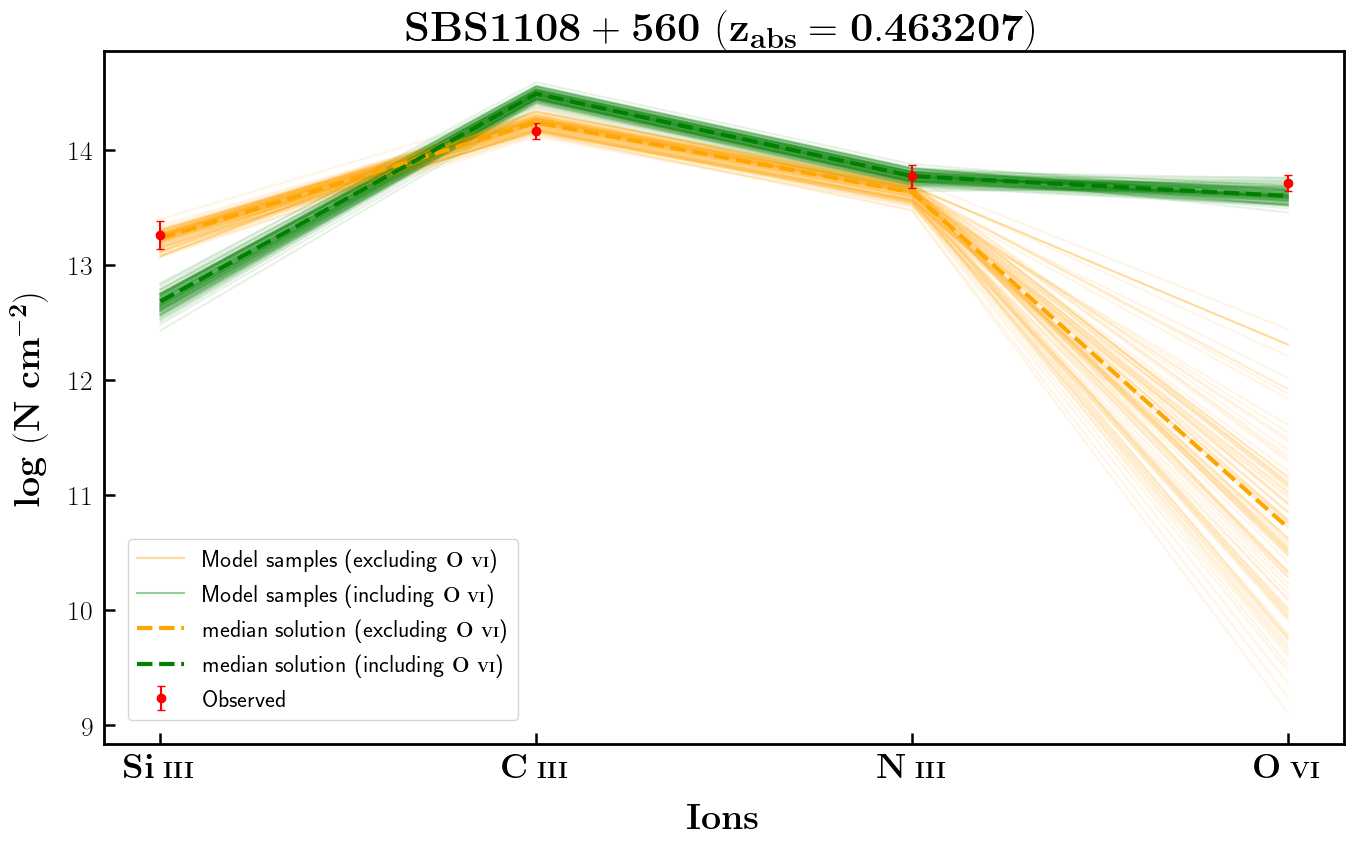
\includegraphics[width=0.9\linewidth]{Ionisation-Modelling-Plots/sbs1108-z=0.463207-compII_logZ=-1.png}
      \caption{$\log \text{N}(\ion{H}{i}) \ [\text{cm}^{-2}]=$ 15.79}
  \end{figure}
  
  
  \newpage
  \thispagestyle{empty}

  \begin{landscape}
  
  \begin{figure}
      \centering
      \vspace{-10mm}
      \hspace*{-20mm}
      \captionsetup{oneside,margin={0cm,20mm}}
      \includegraphics[width=1.1\linewidth]{System-Plots/PG1222+216_z=0.378389_sys_plot.png}
      \caption{System plot for the absorber along the LOS of PG 1222+216 at $z_{abs} = 0.378389$. }
  \end{figure}
  
  \end{landscape}
  
  
  \begin{center} 
  
  \begin{tabular}{cccc} 
  
      \hline \hline \tabularnewline 
      \head{Ion} & \head{v (km s\textsuperscript{$\mathbf{-1}$})} & \head{b (km s\textsuperscript{$\mathbf{-1}$})} & \head{log [N cm\textsuperscript{$\mathbf{-2}$}]}
      \tabularnewline \tabularnewline \hline \tabularnewline 
   
      \ion{O}{iii}   &    7 $\pm$ 5    &    61 $\pm$ 8    &     14.51 $\pm$ 0.04 \\
      \ion{Si}{iii}   &    0 $\pm$ 2    &    30 $\pm$ 3    &     12.98 $\pm$ 0.03 \\
      \ion{C}{iii}   &    -261 $\pm$ 3    &    17 $\pm$ 5    &     13.54 $\pm$ 0.06 \\
      \ion{C}{iii}   &    -215 $\pm$ 5    &    22 $\pm$ 6    &     13.40 $\pm$ 0.08 \\
      \ion{C}{iii}   &    0 $\pm$ 2    &    32 $\pm$ 3    &     13.79 $\pm$ 0.02 \\
      \ion{C}{iii}   &    63 $\pm$ 3    &    13 $\pm$ 6    &     13.12 $\pm$ 0.07 \\
      \ion{O}{vi}   &    -439 $\pm$ 3    &    28 $\pm$ 5    &     13.42 $\pm$ 0.06 \\
      \ion{O}{vi}   &    -264 $\pm$ 6    &    24 $\pm$ 6    &     13.75 $\pm$ 0.2 \\
      \ion{O}{vi}   &    -223 $\pm$ 14    &    34 $\pm$ 13    &     13.68 $\pm$ 0.24 \\
      \ion{O}{vi}   &    -24 $\pm$ 12    &    14 $\pm$ 18    &     13.00 $\pm$ 0.11 \\
      \ion{O}{vi}   &    13 $\pm$ 4    &    29 $\pm$ 13    &     13.95 $\pm$ 0.16 \\
      \ion{O}{vi}   &    59 $\pm$ 6    &    18 $\pm$ 7    &     13.42 $\pm$ 0.23 \\
      \ion{H}{i}   &    -455 $\pm$ 3    &    26 $\pm$ 4    &     13.40 $\pm$ 0.06 \\
      \ion{H}{i}   &    -353 $\pm$ 9    &    64 $\pm$ 19    &     13.54 $\pm$ 0.11 \\
      \ion{H}{i}   &    -268 $\pm$ 1    &    16 $\pm$ 6    &     13.70 $\pm$ 0.14 \\
      \ion{H}{i}   &    -227 $\pm$ 5    &    52 $\pm$ 4    &     14.34 $\pm$ 0.05 \\
      \ion{H}{i}   &    -27 $\pm$ 2    &    23 $\pm$ 1    &     14.73 $\pm$ 0.08 \\
      \ion{H}{i}   &    31 $\pm$ 2    &    43 $\pm$ 1    &     15.43 $\pm$ 0.04 \\
      
      \tabularnewline \hline \hline \tabularnewline 
  
  \end{tabular}
  
  \end{center}
  
  $\log \text{N}(\ion{H}{i}) \ [\text{cm}^{-2}]=$ 15.43 \\
  
  Excluding \ion{O}{vi} : $\log n_H \ (\text{cm}^{-3})$ = -2.66 $\pm$ 0.05 \hspace{10mm} $\log \ Z/Z_\odot$ = -0.25 $\pm$ 0.06
  
  Including \ion{O}{vi} : $\log n_H \ (\text{cm}^{-3})$ = -3.16 $\pm$ 0.03 \hspace{10mm} $\log \ Z/Z_\odot$ = -0.66 $\pm$ 0.02
  
  \newpage
  
  \begin{figure}[!h]
    \centering
    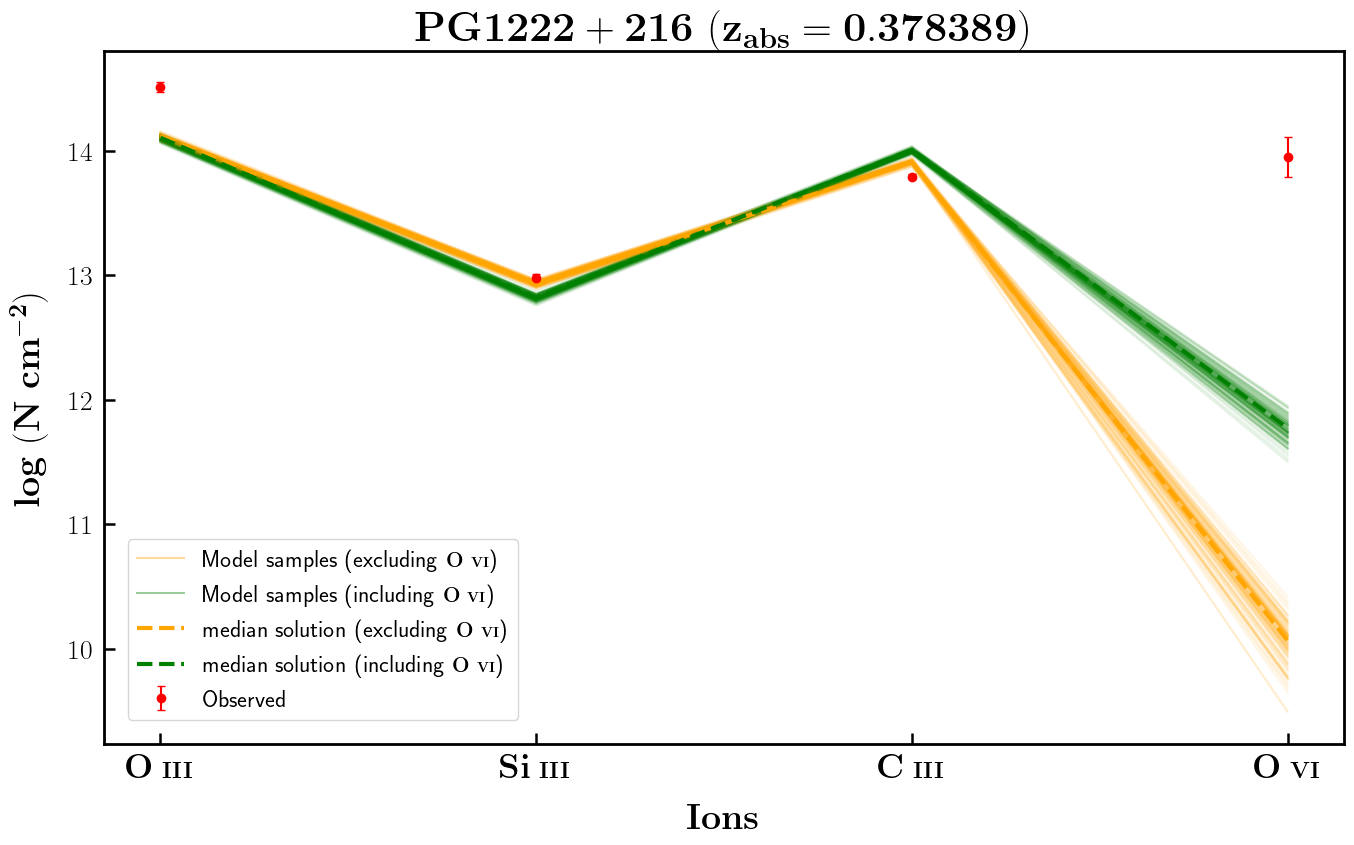
\includegraphics[width=0.9\linewidth]{Ionisation-Modelling-Plots/pg1222-z=0.378389-compVI.png}
    \caption{$\log \text{N}(\ion{H}{i}) \ [\text{cm}^{-2}]=$ 15.43}
  \end{figure}
  
  
  \newpage
  \thispagestyle{empty}

  \begin{landscape}
  
  \begin{figure}
      \centering
      \vspace{-10mm}
      \hspace*{-20mm}
      \captionsetup{oneside,margin={0cm,20mm}}
      \includegraphics[width=1.1\linewidth]{System-Plots/PG1116+215_z=0.138527_sys_plot.png}
      \caption{System plot for the absorber along the LOS of PG 1116+215 at $z_{abs} = 0.138527$. }
  \end{figure}
  
  \end{landscape}
  
  \newgeometry{top=20mm,bottom=0.1cm}
  
  \begin{center} 
  
  \begin{tabular}{cccc} 
  
      \hline \hline \tabularnewline 
      \head{Ion} & \head{v (km s\textsuperscript{$\mathbf{-1}$})} & \head{b (km s\textsuperscript{$\mathbf{-1}$})} & \head{log [N cm\textsuperscript{$\mathbf{-2}$}]}
      \tabularnewline \tabularnewline \hline \tabularnewline 
   
      \ion{N}{v}   &    -7 $\pm$ 3    &    12 $\pm$ 6    &     12.84 $\pm$ 0.09 \\
      \ion{N}{ii}   &    -5 $\pm$ 1    &    6 $\pm$ 3    &     13.62 $\pm$ 0.11 \\
      \ion{N}{ii}   &    33 $\pm$ 6    &    8 $\pm$ 13    &     12.85 $\pm$ 0.15 \\
      \ion{P}{ii}   &    -44 $\pm$ 5    &    19 $\pm$ 8    &     12.94 $\pm$ 0.09 \\
      \ion{Si}{ii}   &    -13 $\pm$ 1    &    9 $\pm$ 1    &     12.46 $\pm$ 0.06 \\
      \ion{Si}{ii}   &    13 $\pm$ 1    &    23 $\pm$ 3    &     12.31 $\pm$ 0.04 \\
      \ion{Si}{iii}   &    -9 $\pm$ 1    &    10 $\pm$ 1    &     12.92 $\pm$ 0.04 \\
      \ion{Si}{iv}   &    -13 $\pm$ 2    &    4 $\pm$ 3    &     12.84 $\pm$ 0.09 \\
      \ion{O}{vi}   &    -1 $\pm$ 1    &    35 $\pm$ 3    &     13.84 $\pm$ 0.02 \\
      \ion{C}{iv}   &    -10 $\pm$ 3    &    13 $\pm$ 4    &     13.17 $\pm$ 0.07 \\
      \ion{C}{ii}   &    -7 $\pm$ 1    &    9 $\pm$ 1    &     13.85 $\pm$ 0.04 \\
      \ion{H}{i}   &    -8 $\pm$ 3    &    27 $\pm$ 2    &     14.97 $\pm$ 0.05 \\
      \ion{H}{i}   &    -5 $\pm$ 9    &    71 $\pm$ 14    &     13.6 $\pm$ 0.23 \\
      \ion{H}{i}   &    31 $\pm$ 2    &    6 $\pm$ 2    &     16.04 $\pm$ 1.77 \\
  
      \tabularnewline \hline \hline \tabularnewline 
  
  \end{tabular}
  
  \end{center}
  
  $\log \text{N}(\ion{H}{i}) \ [\text{cm}^{-2}]=$ 13.60   \\ 
  
  Excluding \ion{O}{vi} : $\log n_H \ (\text{cm}^{-3})$ = -3.24 $\pm$ 0.03 \hspace{10mm} $\log \ Z/Z_\odot$ = 1.92 $\pm$ 0.03
  
  Including \ion{O}{vi} : $\log n_H \ (\text{cm}^{-3})$ = -3.88 $\pm$ 0.01 \hspace{10mm} $\log \ Z/Z_\odot$ = 1.87 $\pm$ 0.02 \\
  
  
%   \newpage 
  
  \begin{figure}[!h]
      \centering
      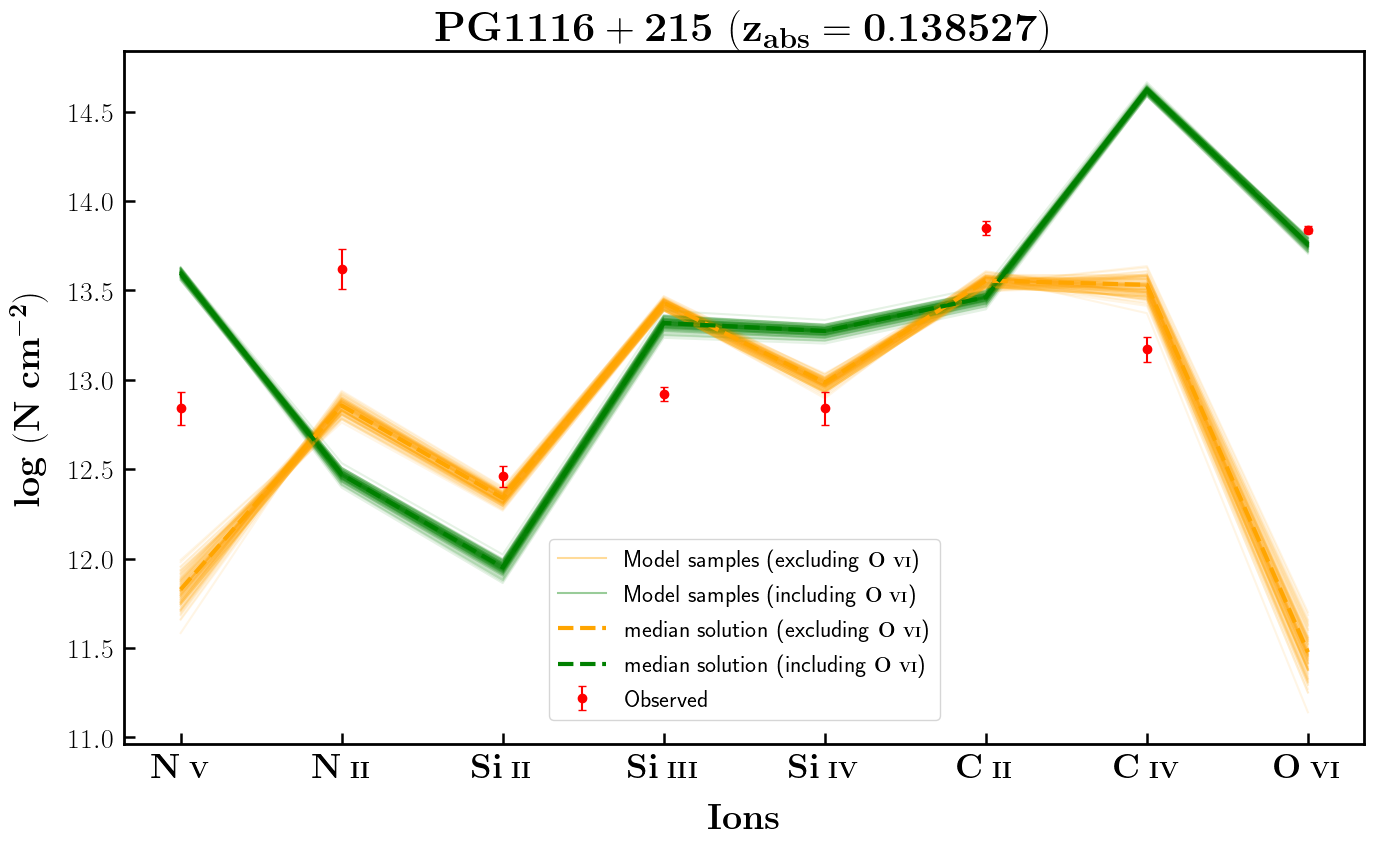
\includegraphics[width=0.9\linewidth]{Ionisation-Modelling-Plots/pg1116-z=0.138527-compII_logZ=-1.png}
      \caption{$\log \text{N}(\ion{H}{i}) \ [\text{cm}^{-2}]=$ 13.60}
  \end{figure}
  
  \restoregeometry
  
  \newpage
  \thispagestyle{empty}

  \begin{landscape}
  
  \begin{figure}
      \centering
      \vspace{-10mm}
      \hspace*{-20mm}
      \captionsetup{oneside,margin={0cm,20mm}}
      \includegraphics[width=1.1\linewidth]{System-Plots/H1821+643_z=0.170006_sys_plot.png}
      \caption{System plot for the absorber along the LOS of H 1821+643 at $z_{abs} = 0.170006$. }
  \end{figure}
  
  \end{landscape}
  
  
  \begin{center} 
  
  \begin{tabular}{cccc} 
  
      \hline \hline \tabularnewline 
      \head{Ion} & \head{v (km s\textsuperscript{$\mathbf{-1}$})} & \head{b (km s\textsuperscript{$\mathbf{-1}$})} & \head{log [N cm\textsuperscript{$\mathbf{-2}$}]}
      \tabularnewline \tabularnewline \hline \tabularnewline 
   
      \ion{Si}{iii}   &    7 $\pm$ 3    &    17 $\pm$ 5    &     12.05 $\pm$ 0.07 \\
      \ion{Si}{iii}   &    52 $\pm$ 6    &    14 $\pm$ 10    &     11.62 $\pm$ 0.17 \\
      \ion{N}{v}   &    47 $\pm$ 3    &    31 $\pm$ 5    &     13.29 $\pm$ 0.05 \\
      \ion{N}{v}   &    122 $\pm$ 7    &    21 $\pm$ 11    &     12.74 $\pm$ 0.14 \\
      \ion{O}{vi}   &    3 $\pm$ 28    &    152 $\pm$ 20    &     13.94 $\pm$ 0.06 \\
      \ion{O}{vi}   &    107 $\pm$ 9    &    48 $\pm$ 12    &     13.29 $\pm$ 0.11 \\
      \ion{H}{i}   &    -92 $\pm$ 1    &    36 $\pm$ 1    &     13.85 $\pm$ 0.02 \\
      \ion{H}{i}   &    0 $\pm$ 2    &    63 $\pm$ 3    &     13.68 $\pm$ 0.02 \\
      \ion{H}{i}   &    120 $\pm$ 1    &    28 $\pm$ 1    &     13.35 $\pm$ 0.02 \\
  
      \tabularnewline \hline \hline \tabularnewline 
  
  \end{tabular}
  
  \end{center}
  
  $\log \text{N}(\ion{H}{i}) \ [\text{cm}^{-2}]=$  13.68  \\ 
  
  Excluding \ion{O}{vi} : $\log n_H \ (\text{cm}^{-3})$ = -4.33 $\pm$ 0.02 \hspace{10mm} $\log \ Z/Z_\odot$ = 1.30 $\pm$ 0.05
  
  Including \ion{O}{vi} : $\log n_H \ (\text{cm}^{-3})$ = -4.43 $\pm$ 0.01 \hspace{10mm} $\log \ Z/Z_\odot$ = 1.25 $\pm$ 0.05
  \\
  
  $\log \text{N}(\ion{H}{i}) \ [\text{cm}^{-2}]=$  13.35  \\ 
  
  Excluding \ion{O}{vi} : $\log n_H \ (\text{cm}^{-3})$ = -4.30 $\pm$ 0.05 \hspace{10mm} $\log \ Z/Z_\odot$ = 1.18 $\pm$ 0.13
  
  Including \ion{O}{vi} : $\log n_H \ (\text{cm}^{-3})$ = -4.41 $\pm$ 0.02 \hspace{10mm} $\log \ Z/Z_\odot$ = 1.15 $\pm$ 0.12
  
  
  \newpage
  
  \begin{figure}[!h]
      \centering
      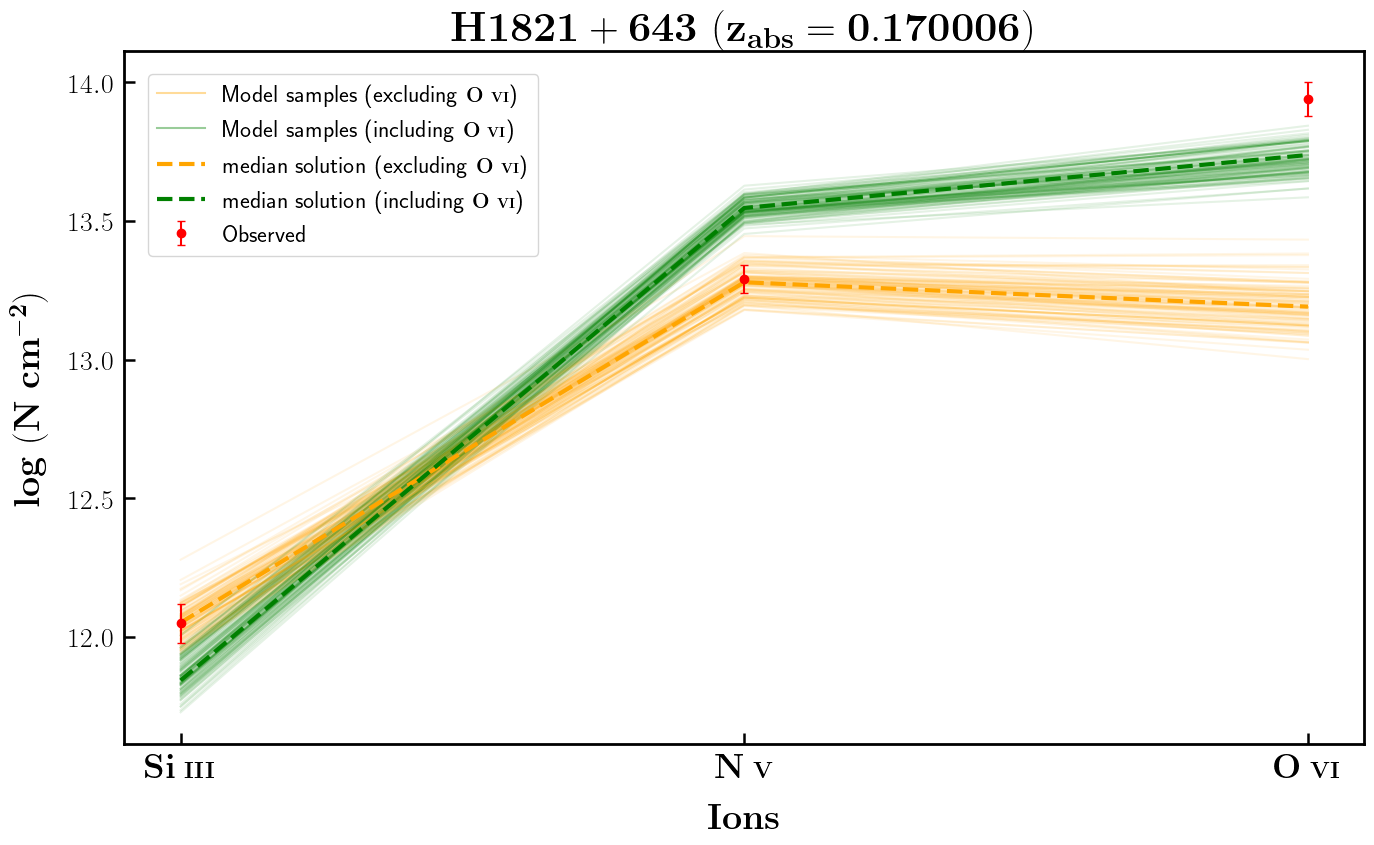
\includegraphics[width=0.9\linewidth]{Ionisation-Modelling-Plots/h1821-z=0.170006-compII.png}
      \caption{$\log \text{N}(\ion{H}{i}) \ [\text{cm}^{-2}]=$ 13.68}
  \end{figure}
  
  \begin{figure}[!b]
      \centering
      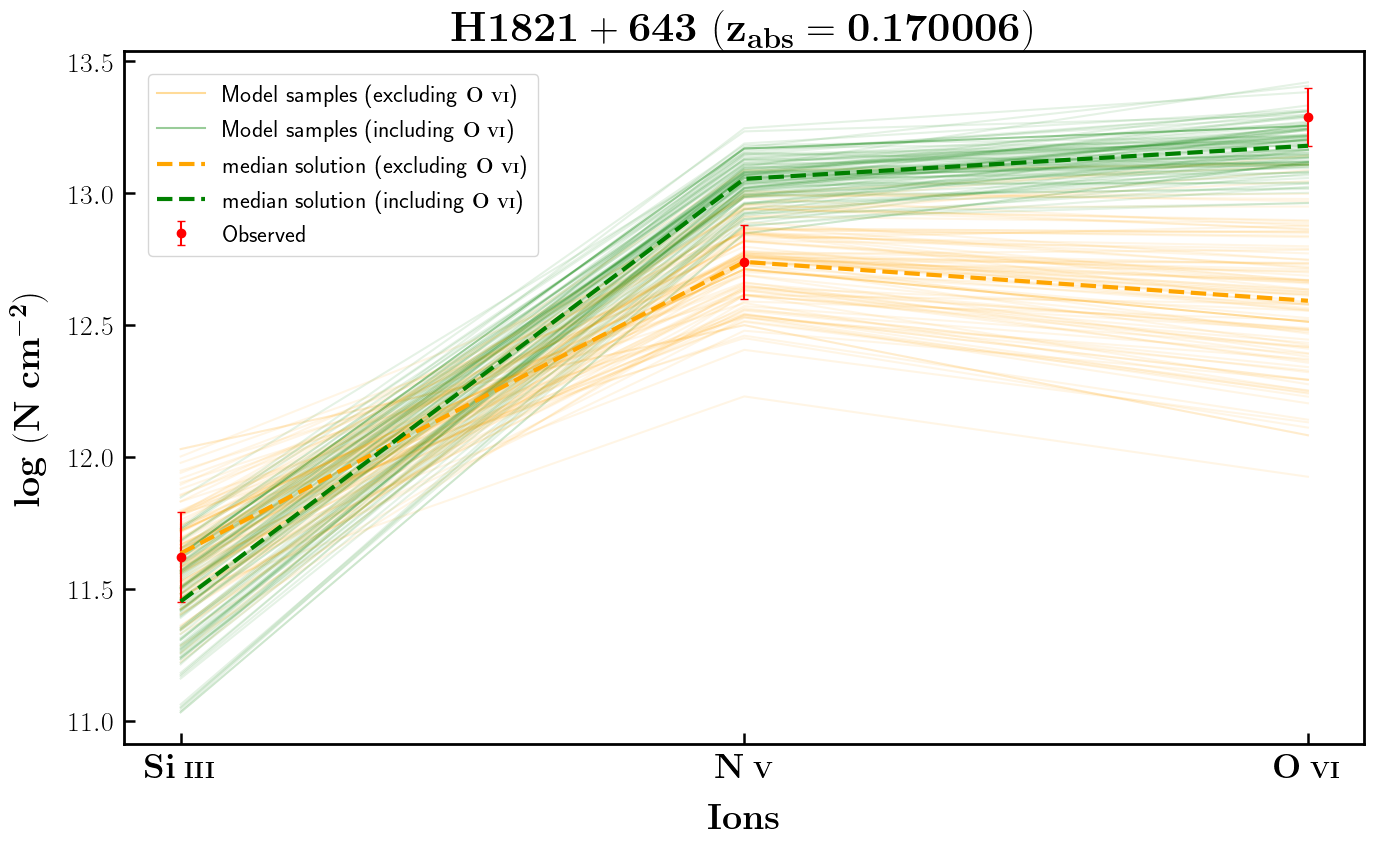
\includegraphics[width=0.9\linewidth]{Ionisation-Modelling-Plots/h1821-z=0.170006-compIII.png}
      \caption{$\log \text{N}(\ion{H}{i}) \ [\text{cm}^{-2}]=$ 13.35}
  \end{figure}
  
  
  \newpage
  \thispagestyle{empty}

  \begin{landscape}
  
  \begin{figure}
      \centering
      \vspace{-10mm}
      \hspace*{-20mm}
      \captionsetup{oneside,margin={0cm,20mm}}
      \includegraphics[width=1.1\linewidth]{System-Plots/H1821+643_z=0.224981_sys_plot.png}
      \caption{System plot for the absorber along the LOS of H 1821+643 at $z_{abs} = 0.224981$. }
  \end{figure}
  
  \end{landscape}
  
  
  \begin{center} 
  
  \begin{tabular}{cccc} 
  
      \hline \hline \tabularnewline 
      \head{Ion} & \head{v (km s\textsuperscript{$\mathbf{-1}$})} & \head{b (km s\textsuperscript{$\mathbf{-1}$})} & \head{log [N cm\textsuperscript{$\mathbf{-2}$}]}
      \tabularnewline \tabularnewline \hline \tabularnewline 
   
      \ion{Si}{iii}   &    -59 $\pm$ 13    &    31 $\pm$ 18    &     12.23 $\pm$ 0.15 \\
      \ion{Si}{iii}   &    -1 $\pm$ 6    &    22 $\pm$ 9    &     12.71 $\pm$ 0.13 \\
      \ion{C}{iii}   &    -31 $\pm$ 1    &    24 $\pm$ 2    &     13.36 $\pm$ 0.07 \\
      \ion{C}{iii}   &    12 $\pm$ 1    &    36 $\pm$ 2    &     13.84 $\pm$ 0.02 \\
      \ion{C}{iii}   &    81 $\pm$ 3    &    15 $\pm$ 5    &     12.6 $\pm$ 0.09 \\
      \ion{C}{iii}   &    335 $\pm$ 7    &    20 $\pm$ 10    &     12.13 $\pm$ 0.11 \\
      \ion{O}{vi}   &    0 $\pm$ 1    &    45 $\pm$ 1    &     14.24 $\pm$ 0.01 \\
      \ion{O}{vi}   &    57 $\pm$ 2    &    3 $\pm$ 3    &     13.12 $\pm$ 0.1 \\
      \ion{O}{vi}   &    330 $\pm$ 1    &    13 $\pm$ 2    &     13.42 $\pm$ 0.03 \\
      \ion{H}{i}   &    -109 $\pm$ 3    &    33 $\pm$ 0    &     13.87 $\pm$ 0.09 \\
      \ion{H}{i}   &    -38 $\pm$ 1    &    30 $\pm$ 1    &     15.16 $\pm$ 0.02 \\
      \ion{H}{i}   &    -19 $\pm$ 10   &    84 $\pm$ 13    &     13.64 $\pm$ 0.11 \\
      \ion{H}{i}   &    18 $\pm$ 1    &    19 $\pm$ 1    &     15.13 $\pm$ 0.03 \\
      \ion{H}{i}   &    276 $\pm$ 7    &    62 $\pm$ 11    &     13.48 $\pm$ 0.06 \\
      
      \tabularnewline \hline \hline \tabularnewline 
  
  \end{tabular}
  
  \end{center}
  
  
  $\log \text{N}(\ion{H}{i}) \ [\text{cm}^{-2}]=$  15.16  \\ 
  
  Excluding \ion{O}{vi} : $\log n_H \ (\text{cm}^{-3})$ = -3.29 $\pm$ 0.08 \hspace{10mm} $\log \ Z/Z_\odot$ = -0.95 $\pm$ 0.07
  
  Including \ion{O}{vi} : $\log n_H \ (\text{cm}^{-3})$ = -4.36 $\pm$ 0.02 \hspace{10mm} $\log \ Z/Z_\odot$ = -0.81 $\pm$ 0.04 \\
  
  $\log \text{N}(\ion{H}{i}) \ [\text{cm}^{-2}]=$  15.13  \\ 
  
  Excluding \ion{O}{vi} : $\log n_H \ (\text{cm}^{-3})$ = -3.29 $\pm$ 0.03 \hspace{10mm} $\log \ Z/Z_\odot$ = -0.44 $\pm$ 0.03
  
  Including \ion{O}{vi} : $\log n_H \ (\text{cm}^{-3})$ = -3.83 $\pm$ 0.04 \hspace{10mm} $\log \ Z/Z_\odot$ = -0.77 $\pm$ 0.03 
  
  \newpage
  
  \begin{figure}[!h]
      \centering
      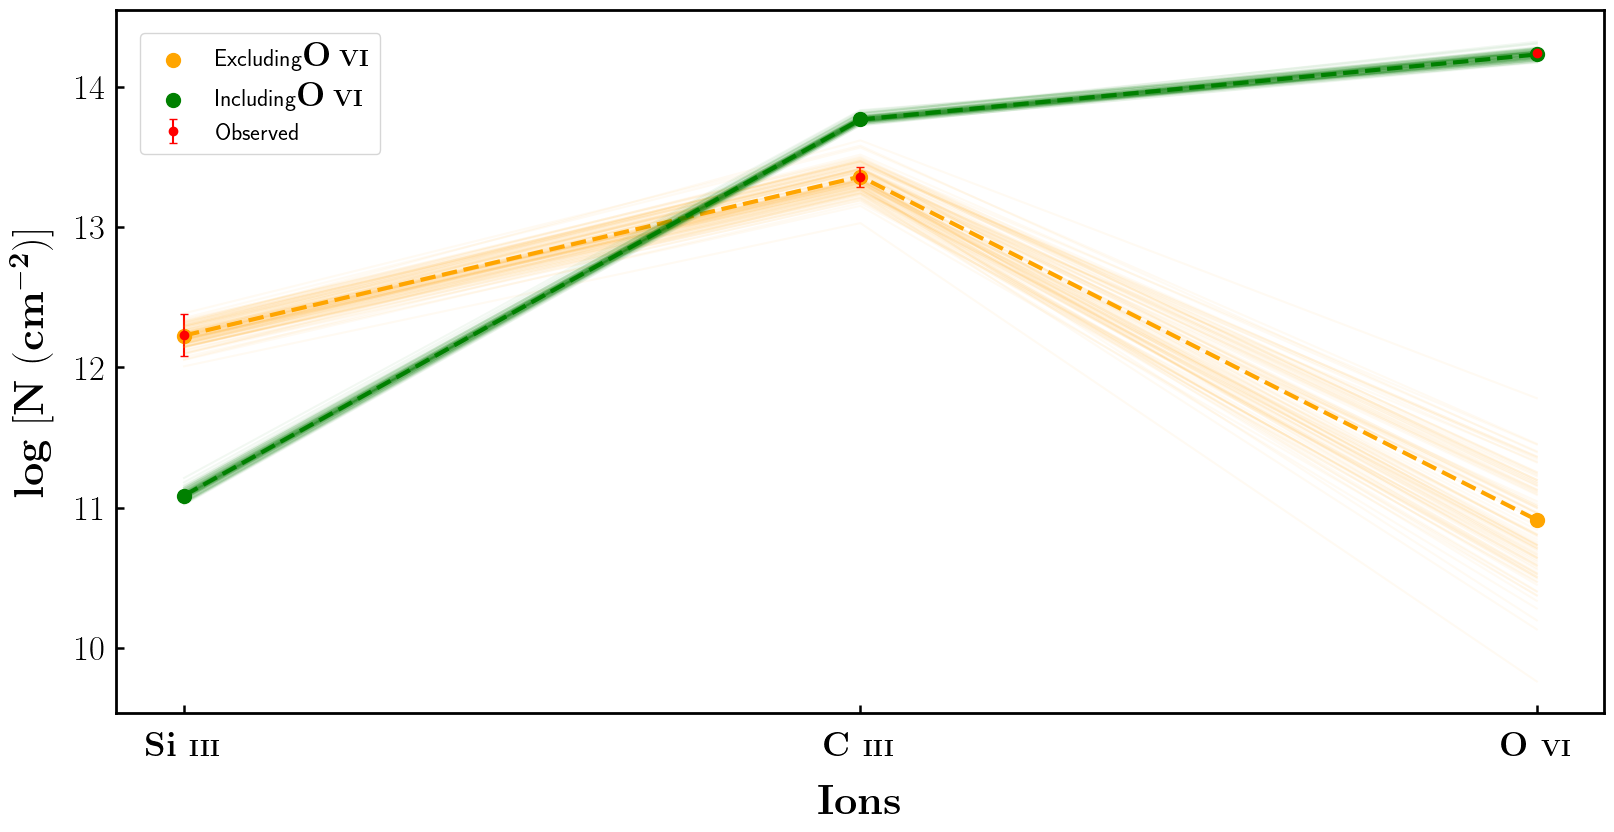
\includegraphics[width=0.9\linewidth]{Ionisation-Modelling-Plots/h1821-z=0.224981-compII.png}
      \caption{$\log \text{N}(\ion{H}{i}) \ [\text{cm}^{-2}]=$ 15.16}
  \end{figure}
  
  \begin{figure}[!b]
      \centering
      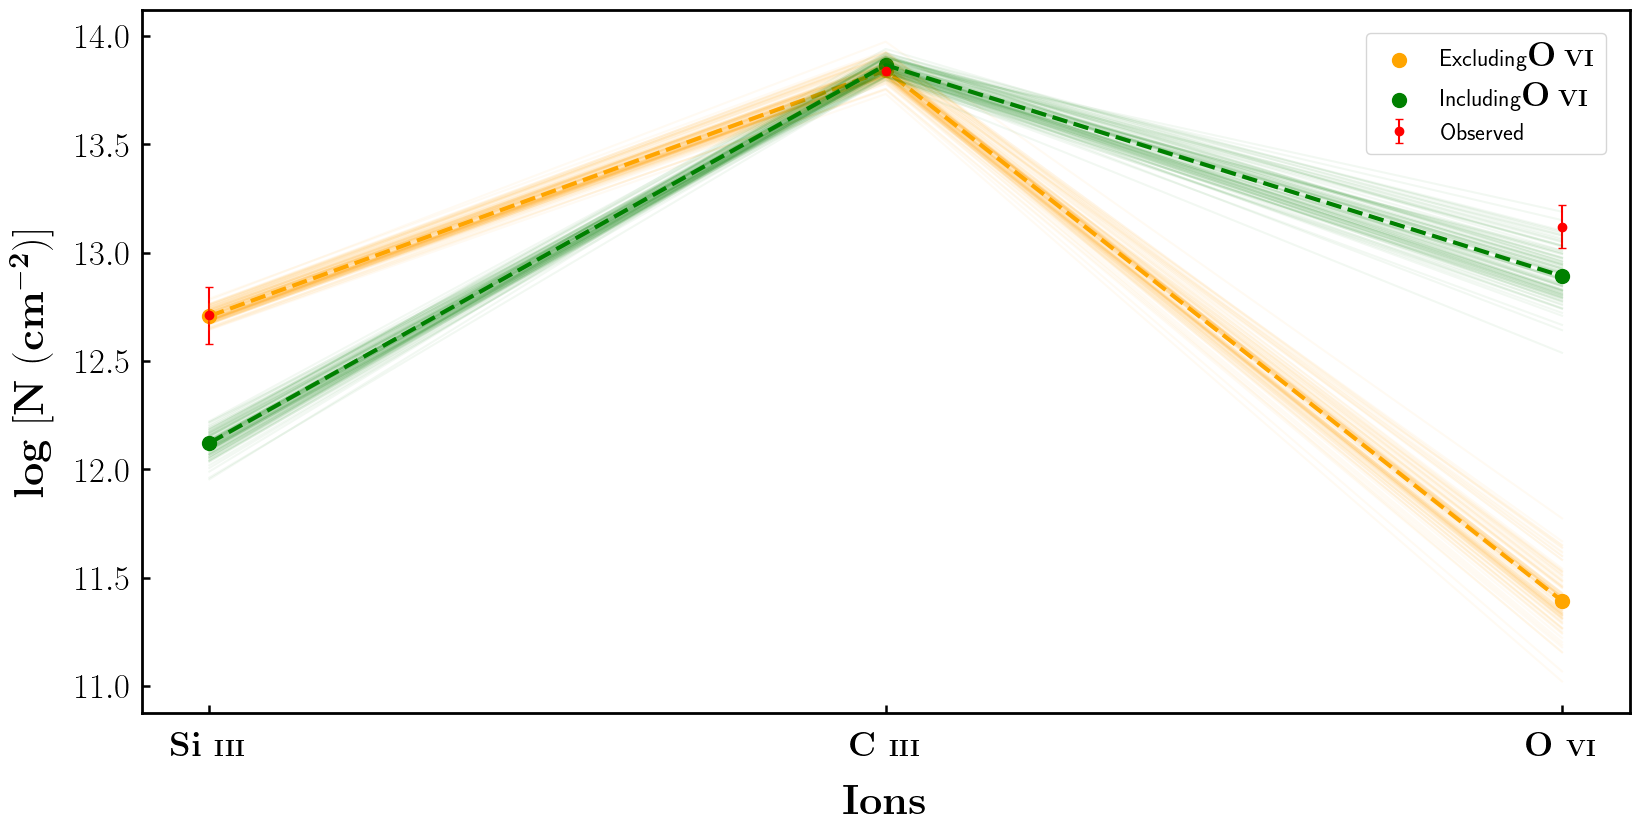
\includegraphics[width=0.9\linewidth]{Ionisation-Modelling-Plots/h1821-z=0.224981-compIV.png}
      \caption{$\log \text{N}(\ion{H}{i}) \ [\text{cm}^{-2}]=$ 15.13}
  \end{figure}
  
  
  
  \newpage
  \thispagestyle{empty}

  \begin{landscape}
  
  \begin{figure}
      \centering
      \vspace{-10mm}
      \hspace*{-20mm}
      \captionsetup{oneside,margin={0cm,20mm}}
      \includegraphics[width=1.1\linewidth]{System-Plots/PG1121+422_z=0.192393_sys_plot.png}
      \caption{System plot for the absorber along the LOS of PG 1121+422 at $z_{abs} = 0.192393$. }
  \end{figure}
  
  \end{landscape}
  
  
  \begin{center} 
  
  \begin{tabular}{cccc} 
  
      \hline \hline \tabularnewline 
      \head{Ion} & \head{v (km s\textsuperscript{$\mathbf{-1}$})} & \head{b (km s\textsuperscript{$\mathbf{-1}$})} & \head{log [N cm\textsuperscript{$\mathbf{-2}$}]}
      \tabularnewline \tabularnewline \hline \tabularnewline 
   
      \ion{Si}{iii}   &    -11 $\pm$ 13    &    10 $\pm$ 3    &     12.62 $\pm$ 0.10 \\
      \ion{Si}{iii}   &    9 $\pm$ 13    &    18 $\pm$ 4    &     13.14 $\pm$ 0.04 \\
      \ion{C}{iii}   &    -26 $\pm$ 10    &    10 $\pm$ 7    &     13.04 $\pm$ 0.09 \\
      \ion{C}{iii}   &    8 $\pm$ 5    &    18 $\pm$ 6    &     13.74 $\pm$ 0.11 \\
      \ion{C}{ii}   &    -9 $\pm$ 3    &    17 $\pm$ 5    &     13.69 $\pm$ 0.08 \\
      \ion{C}{ii}   &    9 $\pm$ 2    &    16 $\pm$ 3    &     13.93 $\pm$ 0.05 \\
      \ion{Si}{iv}   &    10 $\pm$ 7    &    22 $\pm$ 11    &     12.86 $\pm$ 0.13 \\
      \ion{Si}{ii}   &    -3 $\pm$ 1    &    15 $\pm$ 2    &     13.04 $\pm$ 0.06 \\
      \ion{Si}{ii}   &    27 $\pm$ 19    &    42 $\pm$ 1    &     12.48 $\pm$ 0.23 \\
      \ion{O}{vi}   &    -7 $\pm$ 13    &    11 $\pm$ 16    &     12.84 $\pm$ 0.19 \\
      \ion{O}{vi}   &    20 $\pm$ 3    &    3 $\pm$ 4    &     13.37 $\pm$ 0.12 \\
      \ion{H}{i}   &    1 $\pm$ 2    &    60 $\pm$ 6    &     14.34 $\pm$ 0.09 \\
      \ion{H}{i}   &    5 $\pm$ 1    &    19 $\pm$ 1    &     17.7 $\pm$ 0.11 \\
  
      \tabularnewline \hline \hline \tabularnewline 
  
  \end{tabular}
  
  \end{center}
  
  
  $\log \text{N}(\ion{H}{i}) \ [\text{cm}^{-2}]=$ 14.34   \\ 
  
  Excluding \ion{O}{vi} : $\log n_H \ (\text{cm}^{-3})$ = -1.78 $\pm$ 0.05 \hspace{10mm} $\log \ Z/Z_\odot$ = 1.97 $\pm$ 0.04
  
  Including \ion{O}{vi} : $\log n_H \ (\text{cm}^{-3})$ = -3.00 $\pm$ 0.04 \hspace{10mm} $\log \ Z/Z_\odot$ = 1.25 $\pm$ 0.04 \\
  
  $\log \text{N}(\ion{H}{i}) \ [\text{cm}^{-2}]=$  17.70  
  
  Excluding \ion{O}{vi} : $\log n_H \ (\text{cm}^{-3})$ = -2.35 $\pm$ 0.05 \hspace{10mm} $\log \ Z/Z_\odot$ = -1.66 $\pm$ 0.06
  
  Including \ion{O}{vi} : $\log n_H \ (\text{cm}^{-3})$ = -3.08 $\pm$ 0.04 \hspace{10mm} $\log \ Z/Z_\odot$ = -2.08 $\pm$ 0.05 
  
  
  \newpage
  
  \begin{figure}[!h]
      \centering
      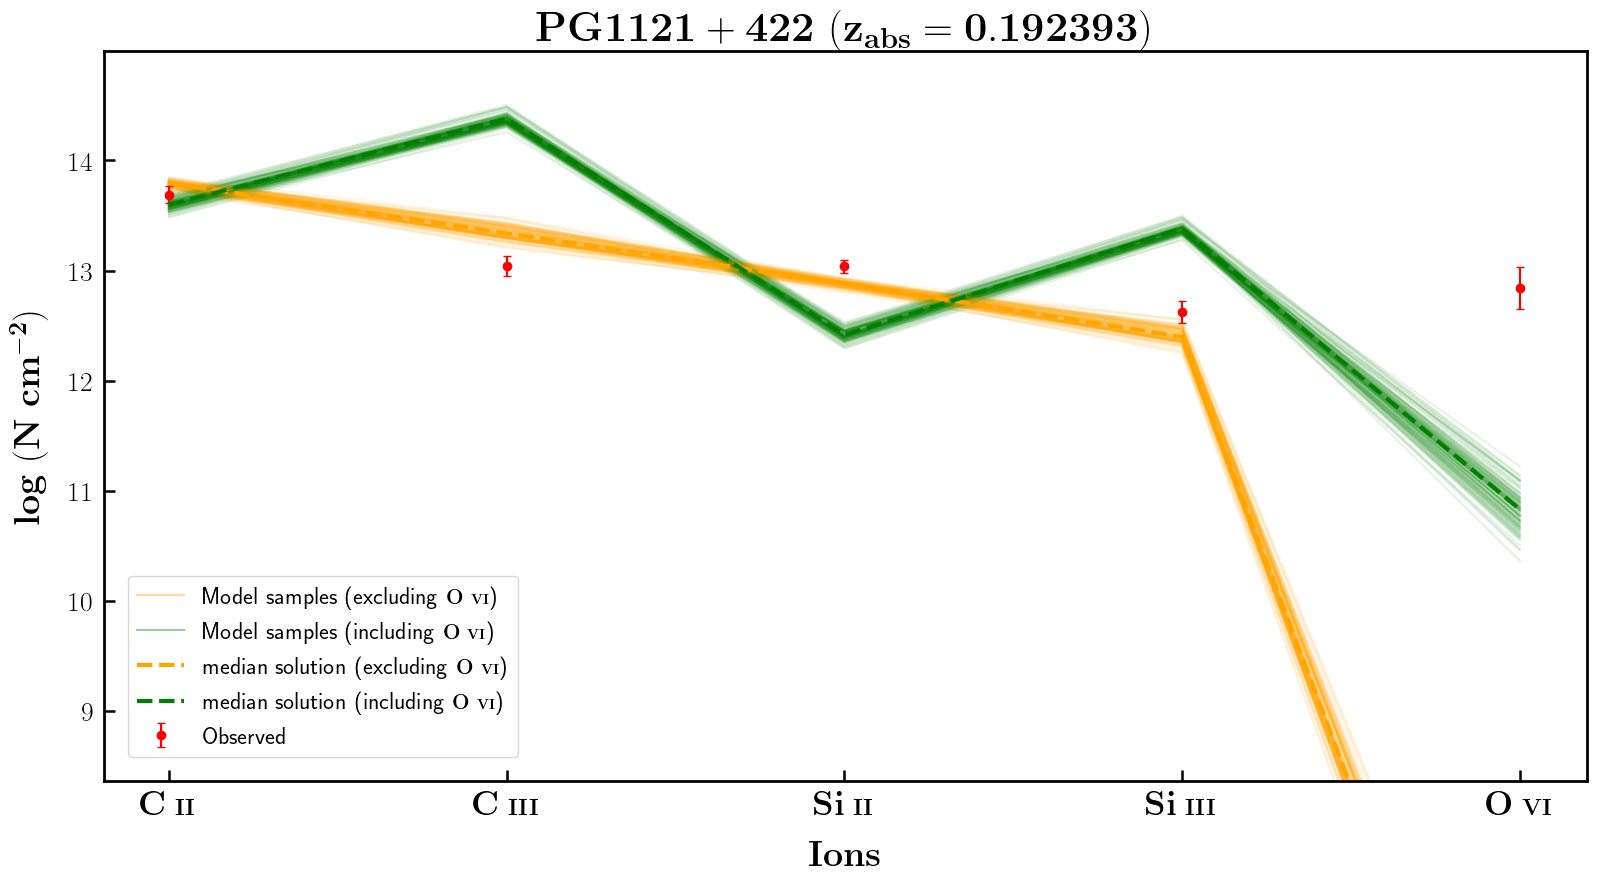
\includegraphics[width=0.9\linewidth]{Ionisation-Modelling-Plots/pg1121-z=0.192393-compI_logZ=-1.png}
      \caption{$\log \text{N}(\ion{H}{i}) \ [\text{cm}^{-2}]=$ 14.34}
  \end{figure}
  
  \begin{figure}[!b]
    \centering
    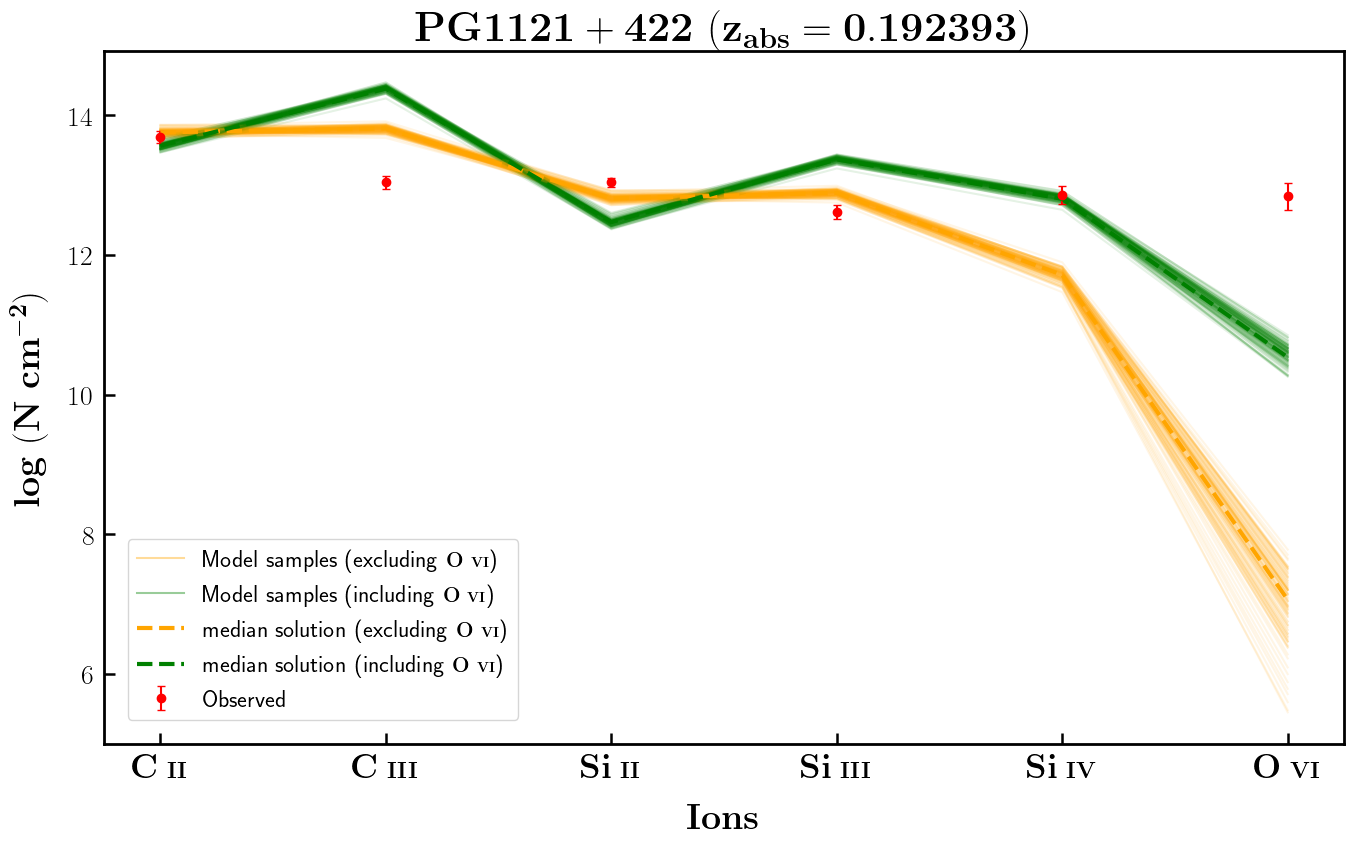
\includegraphics[width=0.9\linewidth]{Ionisation-Modelling-Plots/pg1121-z=0.192393-compII.png}
    \caption{$\log \text{N}(\ion{H}{i}) \ [\text{cm}^{-2}]=$ 17.70}
  \end{figure}
  
  
  
  \newpage
  \thispagestyle{empty}

  \begin{landscape}
  
  \begin{figure}
      \centering
      \vspace{-10mm}
      \hspace*{-20mm}
      \captionsetup{oneside,margin={0cm,20mm}}
      \includegraphics[width=1.1\linewidth]{System-Plots/PKS0405-123_z=0.167125_sys_plot.png}
      \caption{System plot for the absorber along the LOS of PKS 0405-123 at $z_{abs} = 0.167125$. }
  \end{figure}
  
  \end{landscape}

  \newgeometry{top=30mm,bottom=0.1cm}
  
  \begin{center} 
    
%    \begin{table}[H]
%     \centering

  \begin{tabular}{cccc}
  
      \hline \hline \tabularnewline 
      \head{Ion} & \head{v (km s\textsuperscript{$\mathbf{-1}$})} & \head{b (km s\textsuperscript{$\mathbf{-1}$})} & \head{log [N cm\textsuperscript{$\mathbf{-2}$}]}
      \tabularnewline \tabularnewline \hline \tabularnewline 
   
      \ion{O}{i}   &    -14 $\pm$ 5    &    23 $\pm$ 7    &     13.52 $\pm$ 0.08 \\
      \ion{C}{ii}   &    -37 $\pm$ 2    &    16 $\pm$ 2    &     13.76 $\pm$ 0.02 \\
      \ion{C}{ii}   &    -1 $\pm$ 1    &    6 $\pm$ 1    &     16.27 $\pm$ 0.12 \\
      \ion{C}{iii}   &    -136 $\pm$ 2    &    32 $\pm$ 2    &     13.45 $\pm$ 0.02 \\
      \ion{C}{iii}   &    -26 $\pm$ 0    &    37 $\pm$ 2    &     14.33 $\pm$ 0.04 \\
      \ion{N}{ii}   &    -27 $\pm$ 6    &    44 $\pm$ 5    &     13.47 $\pm$ 0.09 \\
      \ion{N}{ii}   &    -7 $\pm$ 1    &    12 $\pm$ 1    &     14.11 $\pm$ 0.02 \\
      \ion{N}{iii}   &    -7 $\pm$ 0    &    9 $\pm$ 4    &     14.06 $\pm$ 0.08 \\
      \ion{N}{iii}   &    5 $\pm$ 0    &    50 $\pm$ 2    &     14.43 $\pm$ 0.02 \\
      \ion{N}{v}   &    -276 $\pm$ 3    &    30 $\pm$ 0    &     13.25 $\pm$ 0.05 \\
      \ion{N}{v}   &    -116 $\pm$ 0    &    59 $\pm$ 9    &     13.32 $\pm$ 0.08 \\
      \ion{N}{v}   &    -79 $\pm$ 13    &    24 $\pm$ 12    &     12.77 $\pm$ 0.19 \\
      \ion{N}{v}   &    -3 $\pm$ 2    &    43 $\pm$ 3    &     13.89 $\pm$ 0.03 \\
      \ion{Si}{iii}   &    -41 $\pm$ 3    &    13 $\pm$ 4    &     12.66 $\pm$ 0.10 \\
      \ion{Si}{iii}   &    -1 $\pm$ 2    &    22 $\pm$ 2    &     13.28 $\pm$ 0.03 \\
      \ion{Si}{iv}   &    -128 $\pm$ 0    &    25 $\pm$ 5    &     12.61 $\pm$ 0.06 \\
      \ion{Si}{iv}   &    2 $\pm$ 1    &    31 $\pm$ 2    &     13.25 $\pm$ 0.02 \\
      \ion{Si}{ii}   &    -48 $\pm$ 5    &    26 $\pm$ 8    &     12.54 $\pm$ 0.09 \\
      \ion{Si}{ii}   &    -4 $\pm$ 1    &    15 $\pm$ 0    &     13.24 $\pm$ 0.02 \\
      \ion{O}{vi}   &    -268 $\pm$ 0    &    74 $\pm$ 5    &     14.05 $\pm$ 0.02 \\
      \ion{O}{vi}   &    -129 $\pm$ 8    &    41 $\pm$ 3    &     14.05 $\pm$ 0.10 \\
      \ion{O}{vi}   &    -64 $\pm$ 5    &    32 $\pm$ 2    &     14.11 $\pm$ 0.17 \\
      \ion{O}{vi}   &    -2 $\pm$ 4    &    43 $\pm$ 3    &     14.49 $\pm$ 0.05 \\
      \ion{H}{i}   &    -158 $\pm$ 0    &    56 $\pm$ 9    &     13.09 $\pm$ 0.06 \\
      \ion{H}{i}   &    -127 $\pm$ 4    &    26 $\pm$ 3    &     13.46 $\pm$ 0.04 \\
      \ion{H}{i}   &    -80 $\pm$ 1    &    18 $\pm$ 2    &     13.54 $\pm$ 0.04 \\
      \ion{H}{i}   &    -30 $\pm$ 0    &    18 $\pm$ 2    &     15.98 $\pm$ 0.34 \\
      \ion{H}{i}   &    8 $\pm$ 49    &    19 $\pm$ 0    &     17.53 $\pm$ 0.07 \\
      \ion{H}{i}   &    54 $\pm$ 90    &    30 $\pm$ 2    &     13.66 $\pm$ 0.04 \\
      
      \tabularnewline \hline \hline 
  
  \end{tabular}
% \end{table} 
  
  \end{center}

  \restoregeometry
  
  $\log \text{N}(\ion{H}{i}) \ [\text{cm}^{-2}]=$  13.46  \\ 
  
  Excluding \ion{O}{vi} : $\log n_H \ (\text{cm}^{-3})$ = -3.98 $\pm$ 0.03 \hspace{10mm} $\log \ Z/Z_\odot$ = 0.62 $\pm$ 0.02
  
  Including \ion{O}{vi} : $\log n_H \ (\text{cm}^{-3})$ = -4.17 $\pm$ 0.02 \hspace{10mm} $\log \ Z/Z_\odot$ = 0.63 $\pm$ 0.02
  \\\\
  
  $\log \text{N}(\ion{H}{i}) \ [\text{cm}^{-2}]=$  15.98  \\ 
  
  Excluding \ion{O}{vi} : $\log n_H \ (\text{cm}^{-3})$ = -2.73 $\pm$ 0.04 \hspace{10mm} $\log \ Z/Z_\odot$ = -0.18 $\pm$ 0.02
  
  Including \ion{O}{vi} : $\log n_H \ (\text{cm}^{-3})$ = -3.27 $\pm$ 0.03 \hspace{10mm} $\log \ Z/Z_\odot$ = -0.33 $\pm$ 0.02
  \\\\
  
  \begin{figure}[!h]
    \centering
    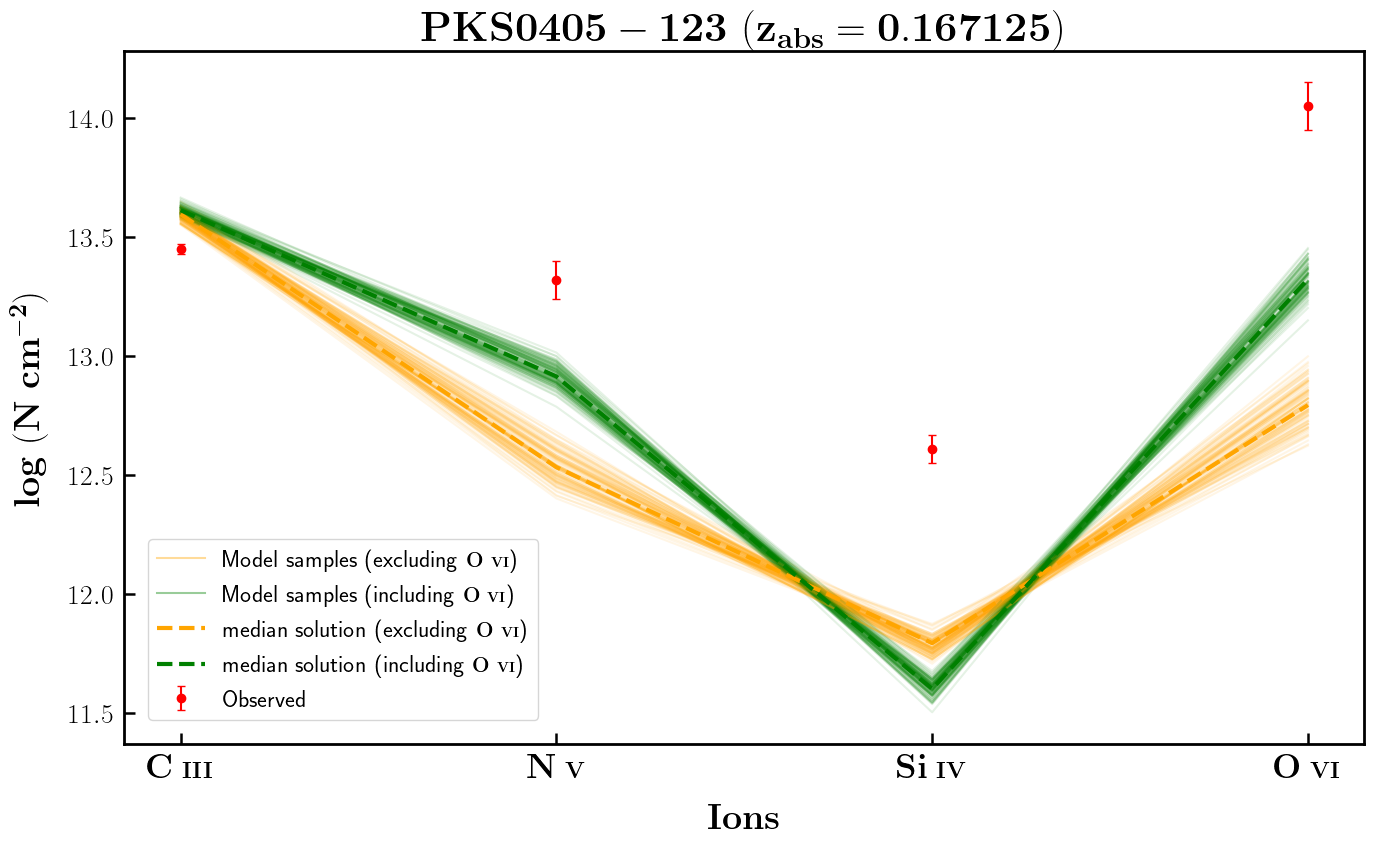
\includegraphics[width=0.9\linewidth]{Ionisation-Modelling-Plots/pks0405-z=0.167125-compII.png}
    \caption{$\log \text{N}(\ion{H}{i}) \ [\text{cm}^{-2}]=$ 13.46}
  \end{figure}
  
  
  \newpage
  
  \begin{figure}[!h]
    \centering
    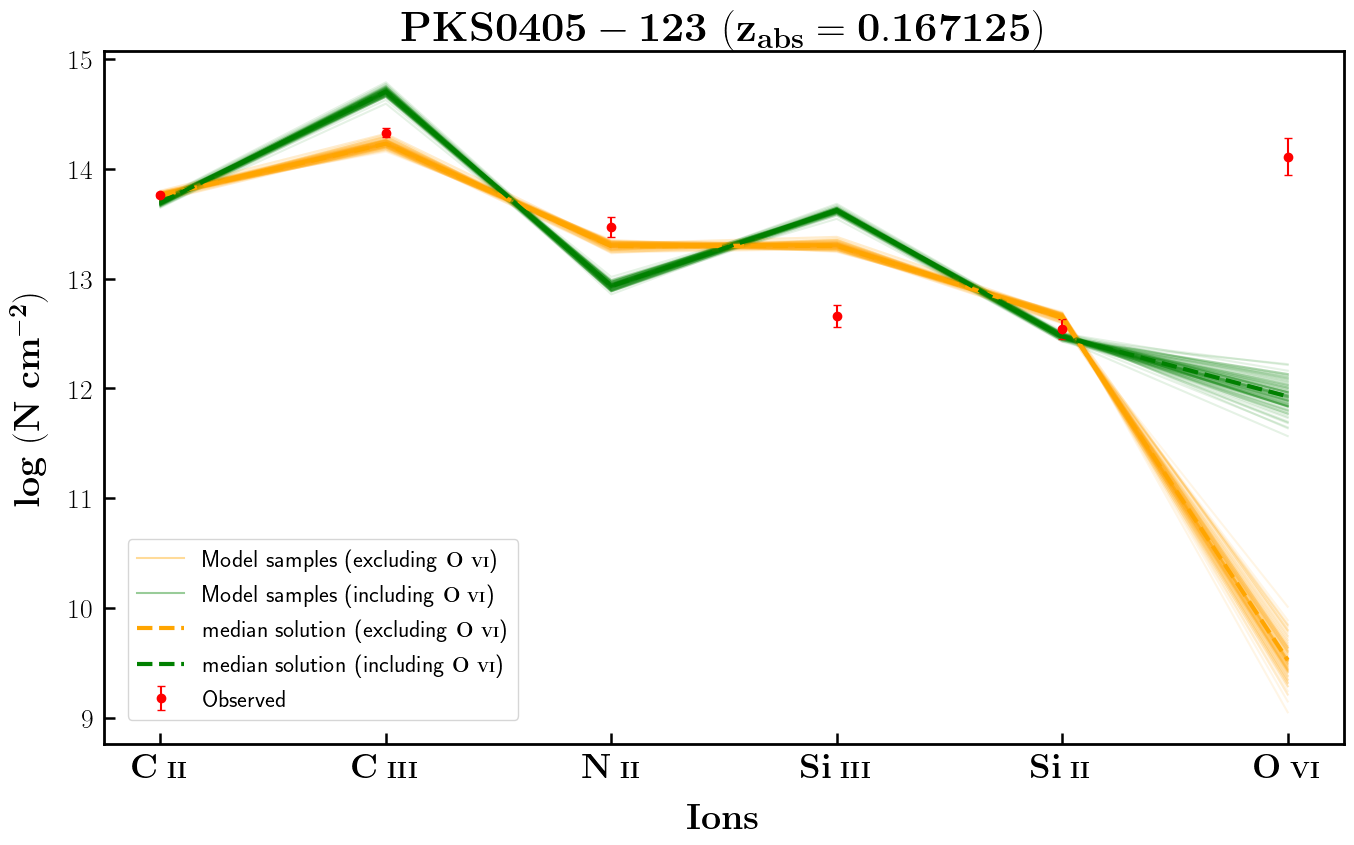
\includegraphics[width=0.9\linewidth]{Ionisation-Modelling-Plots/pks0405-z=0.167125-compIV.png}
    \caption{$\log \text{N}(\ion{H}{i}) \ [\text{cm}^{-2}]=$ 15.98}
  \end{figure}
  
  
  \newpage
  \thispagestyle{empty}

  \begin{landscape}
  
  \begin{figure}
      \centering
      \vspace{-10mm}
      \hspace*{-20mm}
      \captionsetup{oneside,margin={0cm,20mm}}
      \includegraphics[width=1.1\linewidth]{System-Plots/HE0056-3622_z=0.043265_sys_plot.png}
      \caption{System plot for the absorber along the LOS of HE 0056-3622 at $z_{abs} = 0.043265$. }
  \end{figure}
  
  \end{landscape}
  
  
  \begin{center} 
  
  \begin{tabular}{cccc} 
  
      \hline \hline \tabularnewline 
      \head{Ion} & \head{v (km s\textsuperscript{$\mathbf{-1}$})} & \head{b (km s\textsuperscript{$\mathbf{-1}$})} & \head{log [N cm\textsuperscript{$\mathbf{-2}$}]}
      \tabularnewline \tabularnewline \hline \tabularnewline 
   
      \ion{Si}{iii}   &    27 $\pm$ 6   &    34 $\pm$ 9    &     12.37 $\pm$ 0.07 \\
      \ion{N}{v}   &    -26 $\pm$ 4   &    1 $\pm$ 8    &     13.42 $\pm$ 0.46 \\
      \ion{C}{iv}   &    30 $\pm$ 2   &    31 $\pm$ 0    &     13.64 $\pm$ 0.03 \\
      \ion{H}{i}   &    0 $\pm$ 3   &    85 $\pm$ 6    &     14.02 $\pm$ 0.07 \\
      \ion{H}{i}   &    12 $\pm$ 1   &    32 $\pm$ 4    &     15.3 $\pm$ 0.1 \\
  
      \tabularnewline \hline \hline \tabularnewline 
  
  \end{tabular}
  
  \end{center}
  
  $\log \text{N}(\ion{H}{i}) \ [\text{cm}^{-2}]=$  15.30  \\ \hspace*{4mm}
  Solution : $\log n_H \ (\text{cm}^{-3})$ = -4.03 $\pm$ 0.03 \hspace{10mm} $\log \ Z/Z_\odot$ = -0.78 $\pm$ 0.04 \\ 
  
  \begin{figure}[!h]
    \centering
    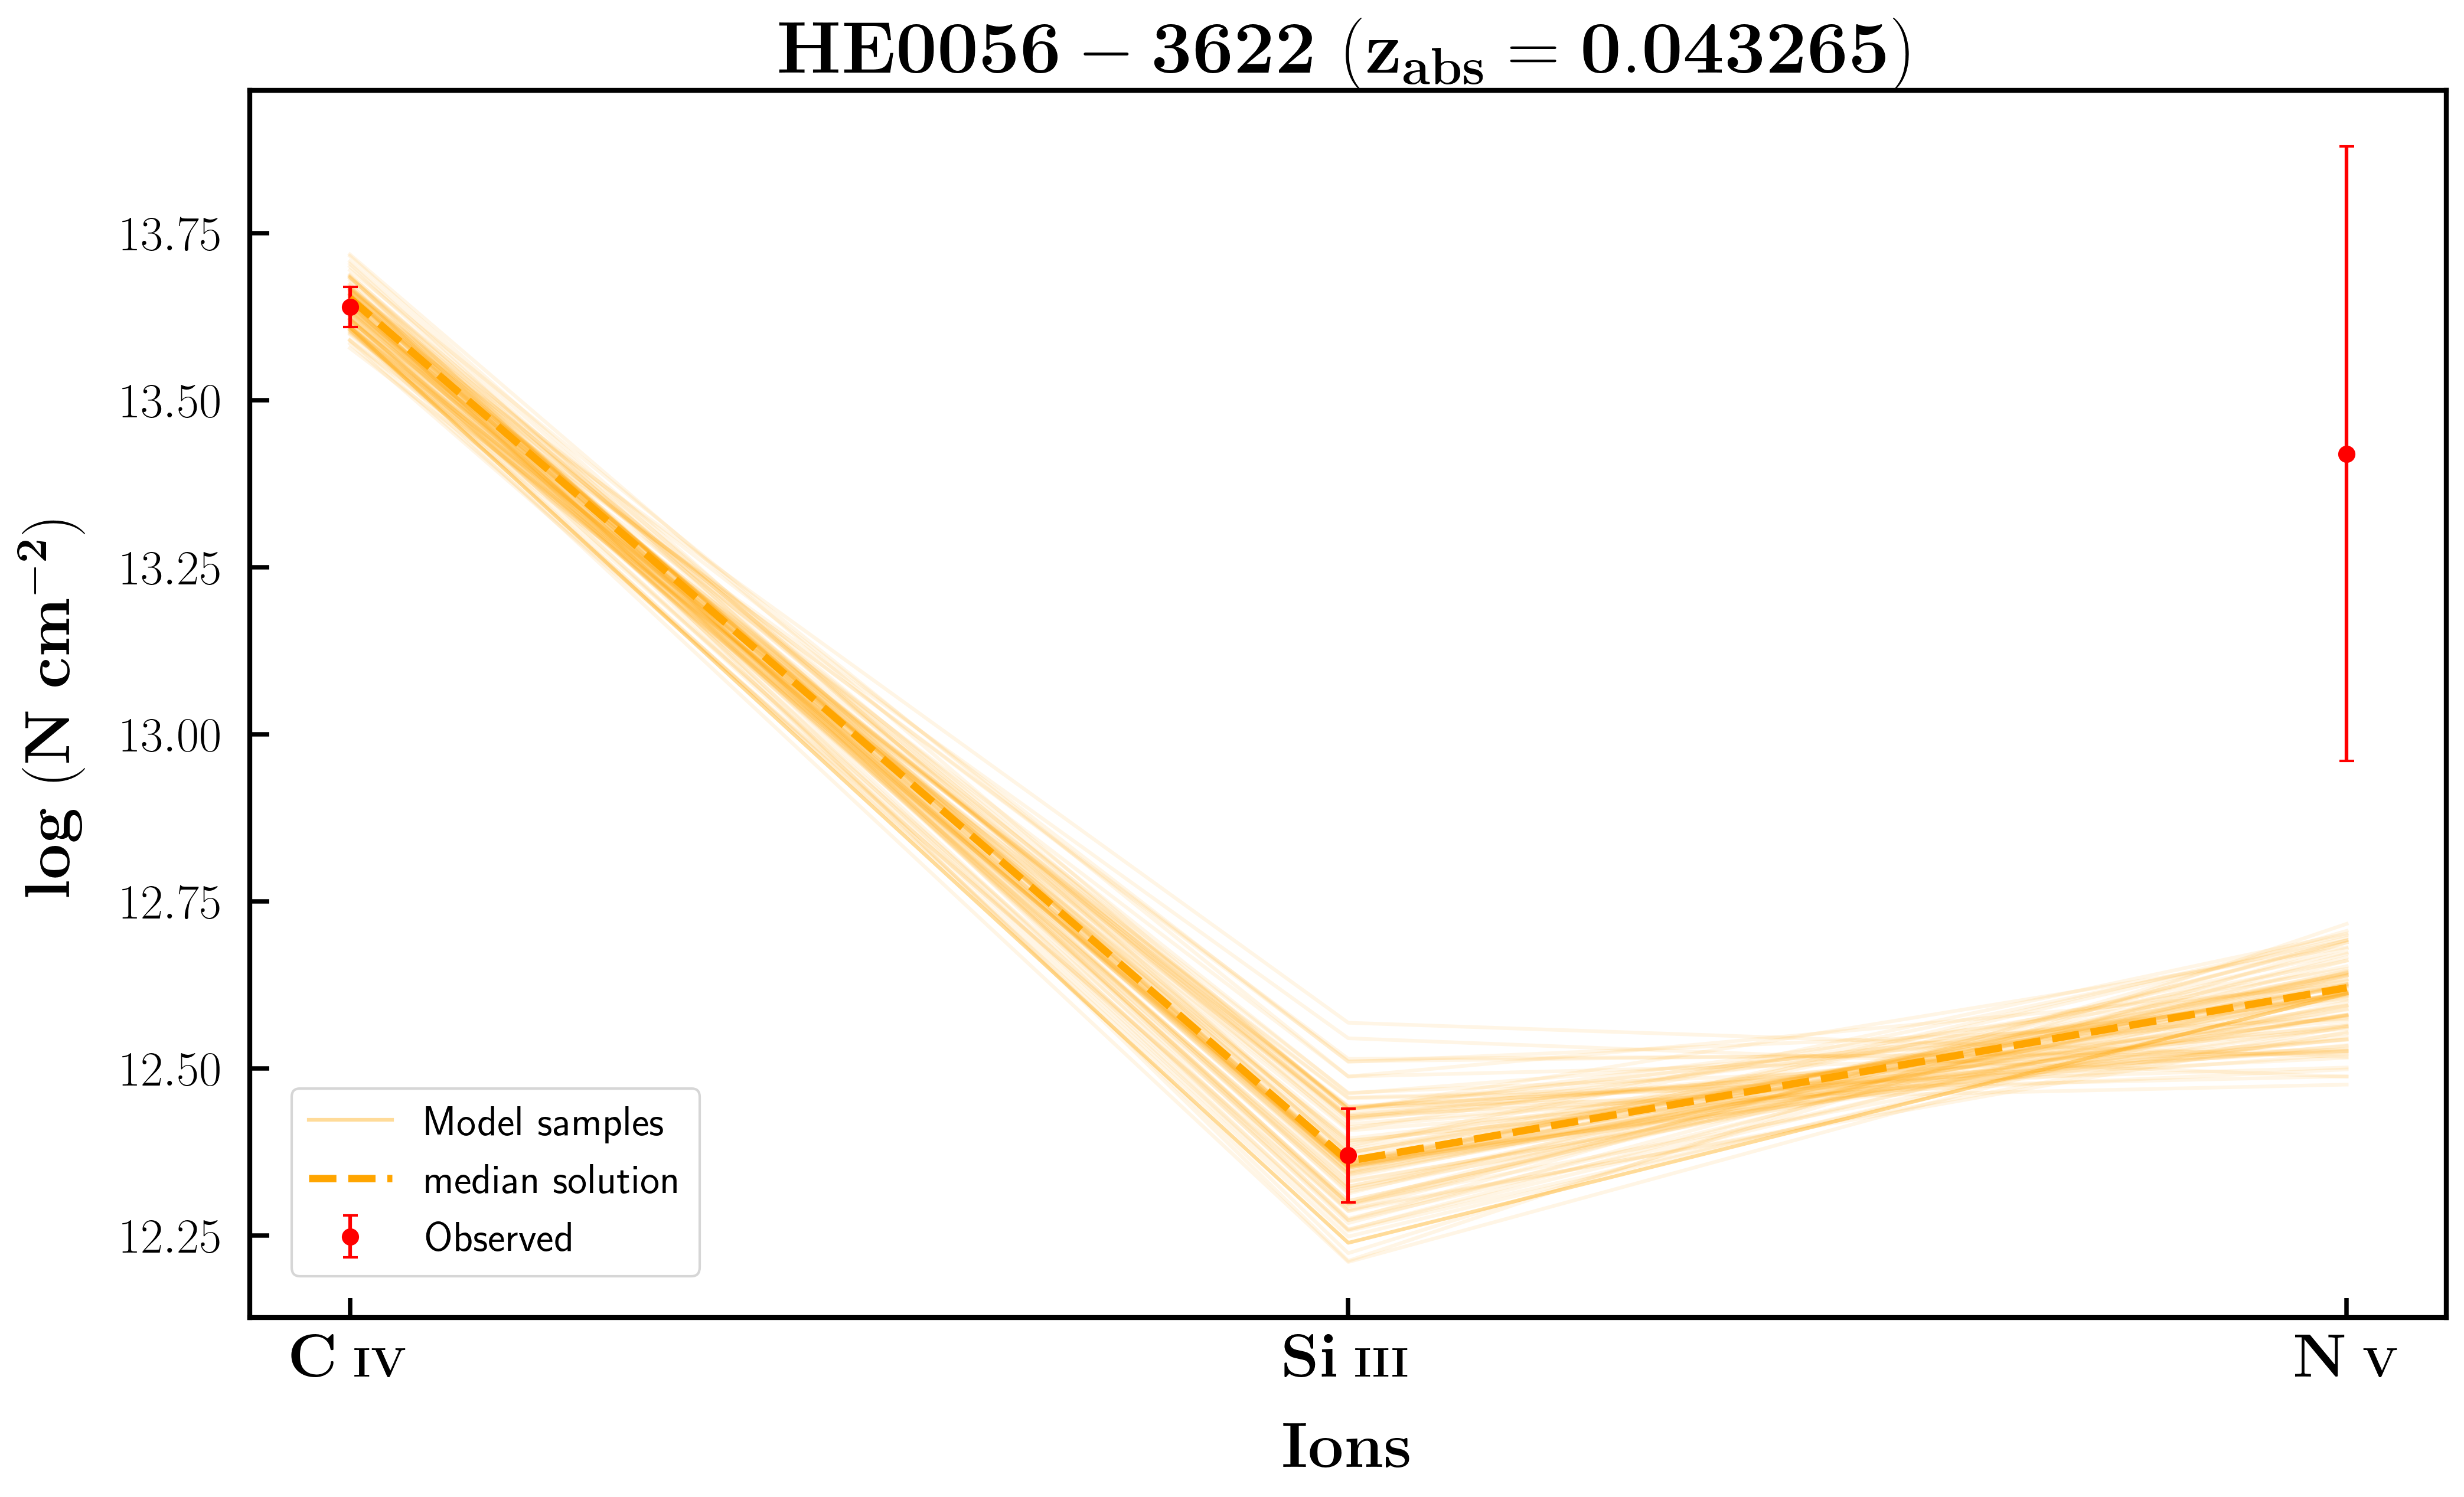
\includegraphics[width=0.9\linewidth]{Ionisation-Modelling-Plots/he0056-z=0.043265-compII_logZ=-1.png}
    \caption{$\log \text{N}(\ion{H}{i}) \ [\text{cm}^{-2}]=$ 15.30}
  \end{figure}
  
  
  \newpage
  \thispagestyle{empty}

  \begin{landscape}
  
  \begin{figure}
      \centering
      \vspace{-10mm}
      \hspace*{-20mm}
      \captionsetup{oneside,margin={0cm,20mm}}
      \includegraphics[width=1.1\linewidth]{System-Plots/PG1216+069_z=0.006328_sys_plot.png}
      \caption{System plot for the absorber along the LOS of PG 1216+069 at $z_{abs} = 0.006328$. }
  \end{figure}
  
  \end{landscape}
  
  \newgeometry{bottom=0.1cm}

  \begin{center} 
  
  \begin{tabular}{cccc} 
  
      \hline \hline \tabularnewline 
      \head{Ion} & \head{v (km s\textsuperscript{$\mathbf{-1}$})} & \head{b (km s\textsuperscript{$\mathbf{-1}$})} & \head{log [N cm\textsuperscript{$\mathbf{-2}$}]}
      \tabularnewline \tabularnewline \hline \tabularnewline 
   
      \ion{O}{i}   &    8 $\pm$ 2   &    7 $\pm$ 5    &     14.07 $\pm$ 0.16 \\
      \ion{O}{i}   &    25 $\pm$ 12   &    50 $\pm$ 13    &     14.0 $\pm$ 0.11 \\
      \ion{C}{ii}   &    0 $\pm$ 3   &    7 $\pm$ 5    &     13.98 $\pm$ 0.08 \\
      \ion{C}{ii}   &    24 $\pm$ 19   &    17 $\pm$ 6    &     13.43 $\pm$ 0.09 \\
      \ion{Si}{ii}   &    -68 $\pm$ 4   &    21 $\pm$ 6    &     12.51 $\pm$ 0.06 \\
      \ion{Si}{ii}   &    6 $\pm$ 1   &    18 $\pm$ 0    &     13.2 $\pm$ 0.02 \\
      \ion{H}{i}   &    -233 $\pm$ 110   &    95 $\pm$ 15    &     13.56 $\pm$ 0.06 \\
      \ion{H}{i}   &    -68 $\pm$ 0   &    81 $\pm$ 8    &     14.76 $\pm$ 0.12 \\
      \ion{H}{i}   &    0 $\pm$ 0   &    106 $\pm$ 15    &     14.79 $\pm$ 0.08 \\
      \ion{H}{i}   &    24 $\pm$ 0   &    20 $\pm$ 12    &     19.09 $\pm$ 0.03 \\
  
      \tabularnewline \hline \hline \tabularnewline 
  
  \end{tabular}
  
  \end{center}
  
  
  $\log \text{N}(\ion{H}{i}) \ [\text{cm}^{-2}]$ = 14.79   \\ \hspace*{4mm}
  Solution : $\log n_H \ (\text{cm}^{-3})$ = -2.69 $\pm$ 0.05 \hspace{10mm} $\log \ Z/Z_\odot$ = 1.97 $\pm$ 0.04 \\ 
  
%   \newpage
  
  \begin{figure}[!h]
    \centering
    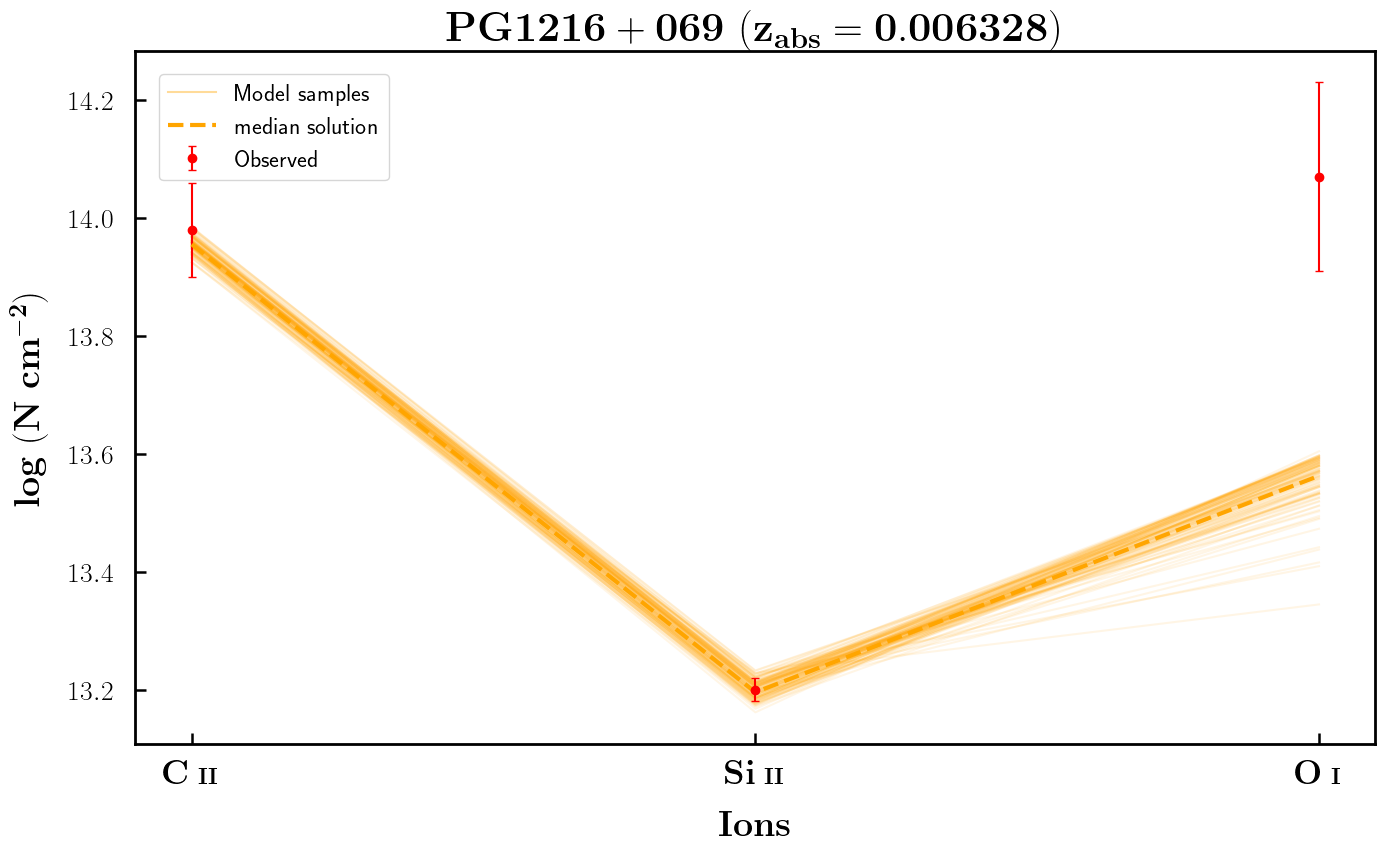
\includegraphics[width=0.9\linewidth]{Ionisation-Modelling-Plots/pg1216-z=0.006328-compIII_logZ=1.png}
    \caption{$\log \text{N}(\ion{H}{i}) \ [\text{cm}^{-2}]=$ 14.79}
  \end{figure}
  
  \restoregeometry
  
  \newpage
  \thispagestyle{empty}

  \begin{landscape}
  
  \begin{figure}
      \centering
      \vspace{-10mm}
      \hspace*{-20mm}
      \captionsetup{oneside,margin={0cm,20mm}}
      \includegraphics[width=1.1\linewidth]{System-Plots/3C263_z=0.063397_sys_plot.png}
      \caption{System plot for the absorber along the LOS of 3C 263 at $z_{abs} = 0.063397$. }
  \end{figure}
  
  \end{landscape}
  
  \newgeometry{bottom=0.1cm}
  
  \begin{center} 
  
  \begin{tabular}{cccc} 
  
      \hline \hline \tabularnewline 
      \head{Ion} & \head{v (km s\textsuperscript{$\mathbf{-1}$})} & \head{b (km s\textsuperscript{$\mathbf{-1}$})} & \head{log [N cm\textsuperscript{$\mathbf{-2}$}]}
      \tabularnewline \tabularnewline \hline \tabularnewline 
   
      \ion{Si}{ii}   &    26 $\pm$ 2   &    8 $\pm$ 4    &     12.29 $\pm$ 0.06 \\
      \ion{Si}{iii}   &    -39 $\pm$ 1   &    21 $\pm$ 2    &     12.64 $\pm$ 0.03 \\
      \ion{Si}{iii}   &    34 $\pm$ 1   &    12 $\pm$ 1    &     12.91 $\pm$ 0.04 \\
      \ion{Si}{iv}   &    25 $\pm$ 1   &    22 $\pm$ 0    &     13.57 $\pm$ 0.02 \\
      \ion{C}{iv}   &    -35 $\pm$ 1   &    12 $\pm$ 3    &     13.42 $\pm$ 0.06 \\
      \ion{C}{iv}   &    0 $\pm$ 2   &    13 $\pm$ 3    &     13.63 $\pm$ 0.06 \\
      \ion{C}{iv}   &    38 $\pm$ 2   &    17 $\pm$ 2    &     13.86 $\pm$ 0.04 \\
      \ion{C}{ii}   &    34 $\pm$ 2   &    17 $\pm$ 3    &     13.37 $\pm$ 0.04 \\
      \ion{H}{i}   &    -146 $\pm$ 2   &    25 $\pm$ 2    &     13.87 $\pm$ 0.04 \\
      \ion{H}{i}   &    -35 $\pm$ 0   &    50 $\pm$ 6    &     14.88 $\pm$ 0.12 \\
      \ion{H}{i}   &    0 $\pm$ 0   &    54 $\pm$ 6    &     14.42 $\pm$ 0.2 \\
      \ion{H}{i}   &    38 $\pm$ 0   &    12 $\pm$ 3    &     16.46 $\pm$ 0.13 \\
  
      \tabularnewline \hline \hline \tabularnewline 
  
  \end{tabular}
  
  \end{center}
  
  
  $\log \text{N}(\ion{H}{i}) \ [\text{cm}^{-2}]$ = 16.46   \\  \hspace*{4mm}
  Solution : $\log n_H \ (\text{cm}^{-3})$ = -3.72 $\pm$ 0.02 \hspace{10mm} $\log \ Z/Z_\odot$ = -0.99 $\pm$ 0.02 \\  
  
%   \newpage 
  
  \begin{figure}[!h]
      \centering
    %   \vspace*{-10mm}
      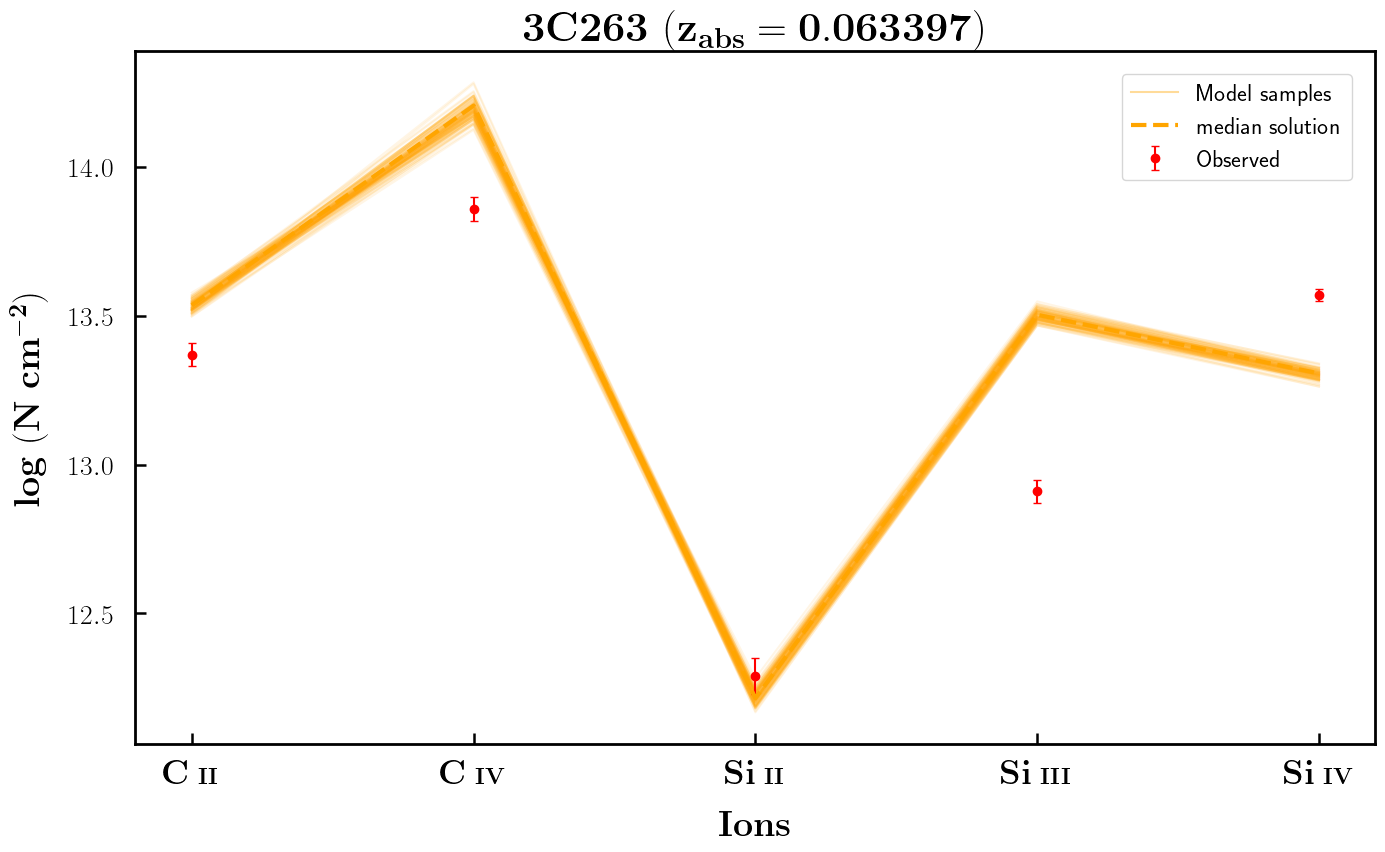
\includegraphics[width=0.9\linewidth]{Ionisation-Modelling-Plots/3c263-z=0.063397-compIV_logZ=-1.png}
      \caption{$\log \text{N}(\ion{H}{i}) \ [\text{cm}^{-2}]=$ 16.46}
  \end{figure}
  
  \restoregeometry
  
  \newpage
  \thispagestyle{empty}

  \begin{landscape}
  
  \begin{figure}
      \centering
      \vspace{-10mm}
      \hspace*{-20mm}
      \captionsetup{oneside,margin={0cm,20mm}}
      \includegraphics[width=1.1\linewidth]{System-Plots/PG1222+216_z=0.054479_sys_plot.png}
      \caption{System plot for the absorber along the LOS of PG 1222+216 at $z_{abs} = 0.054479$. }
  \end{figure}
  
  \end{landscape}
  
  
  \begin{center} 
  
  \begin{tabular}{cccc} 
  
      \hline \hline \tabularnewline 
      \head{Ion} & \head{v (km s\textsuperscript{$\mathbf{-1}$})} & \head{b (km s\textsuperscript{$\mathbf{-1}$})} & \head{log [N cm\textsuperscript{$\mathbf{-2}$}]}
      \tabularnewline \tabularnewline \hline \tabularnewline 
   
      \ion{Si}{iii}   &    -12 $\pm$ 3   &    20 $\pm$ 3    &     13.19 $\pm$ 0.05 \\
      \ion{Si}{iii}   &    40 $\pm$ 5   &    27 $\pm$ 5    &     13.04 $\pm$ 0.07 \\
      \ion{Si}{iv}   &    0 $\pm$ 1   &    25 $\pm$ 8    &     12.89 $\pm$ 0.08 \\
      \ion{Si}{iv}   &    41 $\pm$ 4   &    10 $\pm$ 7    &     12.39 $\pm$ 0.13 \\
      \ion{C}{iv}   &    -2 $\pm$ 1   &    29 $\pm$ 6    &     13.55 $\pm$ 0.1 \\
      \ion{C}{iv}   &    41 $\pm$ 8   &    34 $\pm$ 6    &     13.5 $\pm$ 0.11 \\
      \ion{C}{iv}   &    182 $\pm$ 10   &    26 $\pm$ 15    &     12.86 $\pm$ 0.15 \\
      \ion{C}{ii}   &    7 $\pm$ 4   &    26 $\pm$ 6    &     13.51 $\pm$ 0.07 \\
      \ion{C}{ii}   &    51 $\pm$ 4   &    10 $\pm$ 6    &     12.98 $\pm$ 0.09 \\
      \ion{H}{i}   &    -12 $\pm$ 23   &    74 $\pm$ 11    &     14.08 $\pm$ 0.15 \\
      \ion{H}{i}   &    5 $\pm$ 4   &    24 $\pm$ 3    &     17.91 $\pm$ 0.15 \\
  
      \tabularnewline \hline \hline \tabularnewline 
  
  \end{tabular}
  
  \end{center}
  
  $\log \text{N}(\ion{H}{i}) \ [\text{cm}^{-2}]$ = 14.08 \\ \hspace*{4mm}
  Solution : $\log n_H \ (\text{cm}^{-3})$ = -3.45 $\pm$ 0.06 \hspace{10mm} $\log \ Z/Z_\odot$ = 1.25 $\pm$ 0.05 \\  
  
  $\log \text{N}(\ion{H}{i}) \ [\text{cm}^{-2}]$ = 17.91   \\  \hspace*{4mm}
  Solution : $\log n_H \ (\text{cm}^{-3})$ = -3.86 $\pm$ 0.08 \hspace{10mm} $\log \ Z/Z_\odot$ = -2.91 $\pm$ 0.07 \newline  
  
  \newpage
  
  \begin{figure}[!h]
      \centering
      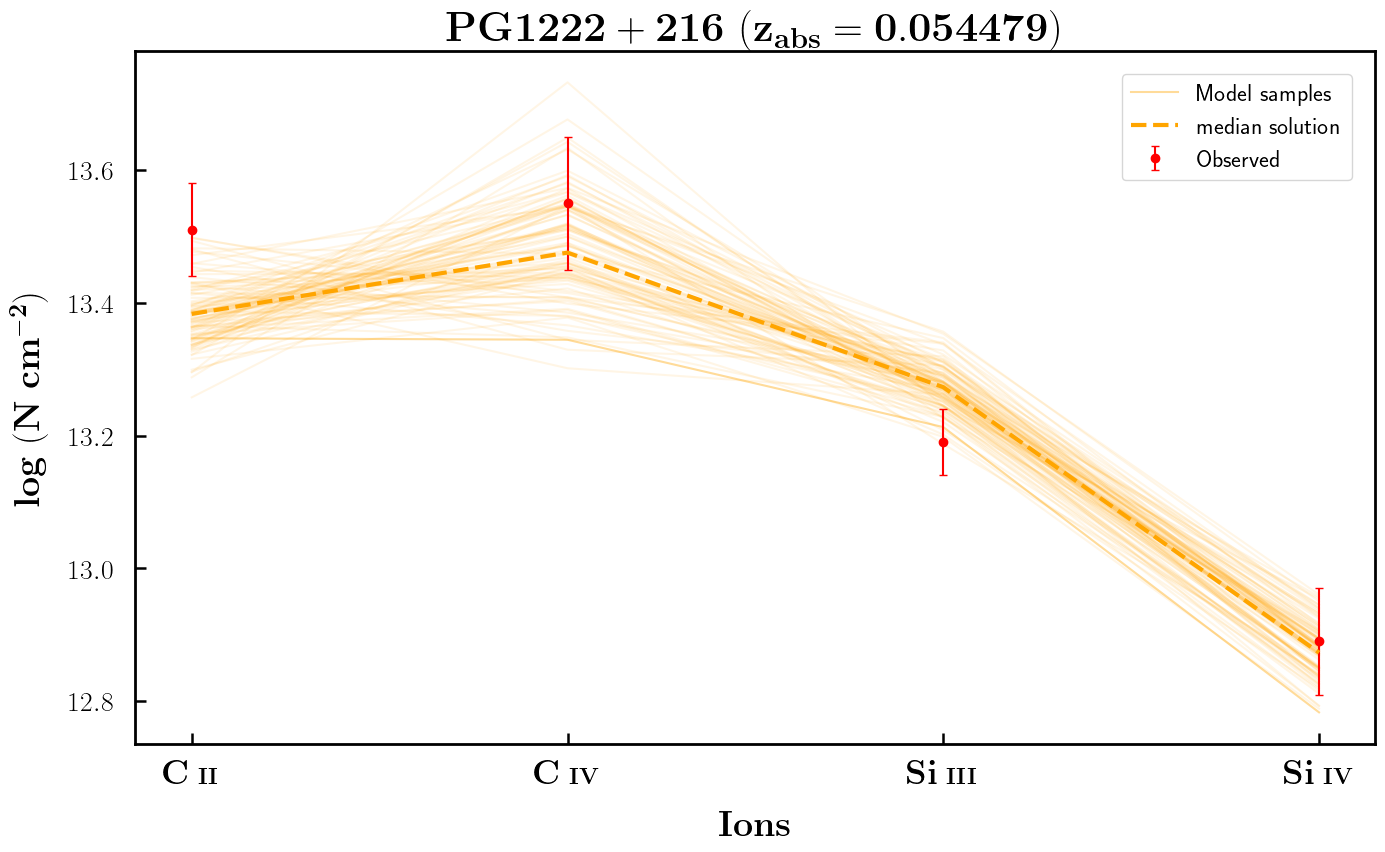
\includegraphics[width=0.9\linewidth]{Ionisation-Modelling-Plots/pg1222-z=0.054479-compI_logZ=-1.png}
      \caption{$\log \text{N}(\ion{H}{i}) \ [\text{cm}^{-2}]=$ 14.08}
  \end{figure}
  
  \begin{figure}[!b]
      \centering
      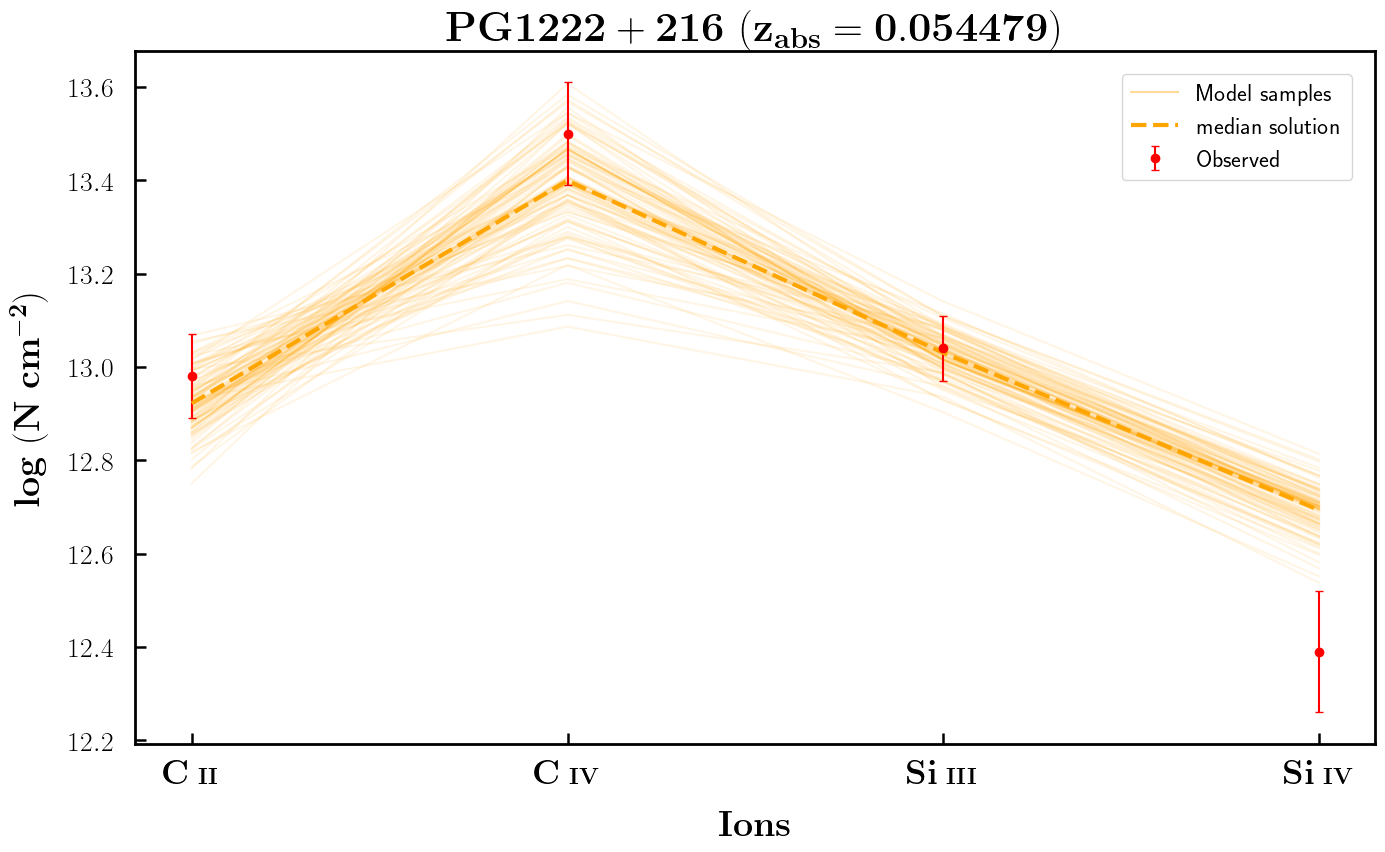
\includegraphics[width=0.9\linewidth]{Ionisation-Modelling-Plots/pg1222-z=0.054479-compII_logZ=-1.png}
      \caption{$\log \text{N}(\ion{H}{i}) \ [\text{cm}^{-2}]=$ 17.91}
  \end{figure}
  
  
  \newpage
  \thispagestyle{empty}

  \begin{landscape}
  
  \begin{figure}
      \centering
      \vspace{-10mm}
      \hspace*{-20mm}
      \captionsetup{oneside,margin={0cm,20mm}}
      \includegraphics[width=1.1\linewidth]{System-Plots/RXJ0439.6-5311_z=0.005568_sys_plot.png}
      \caption{System plot for the absorber along the LOS of RX J0439.6-5311 at $z_{abs} = 0.005568$. }
  \end{figure}
  
  \end{landscape}
  
  
  \begin{center} 
  
  \begin{tabular}{cccc} 
  
      \hline \hline \tabularnewline 
      \head{Ion} & \head{v (km s\textsuperscript{$\mathbf{-1}$})} & \head{b (km s\textsuperscript{$\mathbf{-1}$})} & \head{log [N cm\textsuperscript{$\mathbf{-2}$}]}
      \tabularnewline \tabularnewline \hline \tabularnewline 
   
      \ion{Si}{iii}   &    16 $\pm$ 1   &    11 $\pm$ 3    &     13.01 $\pm$ 0.12 \\
      \ion{Si}{iv}   &    -3 $\pm$ 4   &    20 $\pm$ 6    &     12.77 $\pm$ 0.08 \\
      \ion{C}{iv}   &    4 $\pm$ 3   &    13 $\pm$ 5    &     13.5 $\pm$ 0.07 \\
      \ion{H}{i}   &    0 $\pm$ 2   &    53 $\pm$ 6    &     14.3 $\pm$ 0.09 \\
      \ion{H}{i}   &    5 $\pm$ 3   &    15 $\pm$ 6    &     16.11 $\pm$ 0.26 \\
  
      \tabularnewline \hline \hline \tabularnewline 
  
  \end{tabular}
  
  \end{center}
  
  
  $\log \text{N}(\ion{H}{i}) \ [\text{cm}^{-2}]=$  16.11  \\ \hspace*{4mm}
  Solution : $\log n_H \ (\text{cm}^{-3})$ = -3.69 $\pm$ 0.07 \hspace{10mm} $\log \ Z/Z_\odot$ = -1.07 $\pm$ 0.1 \newline
  
  \begin{figure}[!h]
      \centering
      \includegraphics[width=0.9\linewidth]{Ionisation-Modelling-Plots/rxj0439-z=0.005568-compII_logZ=-1.png}
      \caption{$\log \text{N}(\ion{H}{i}) \ [\text{cm}^{-2}]=$ 16.11}
  \end{figure}
  
  
  
  \newpage
  \thispagestyle{empty}

  \begin{landscape}
  
  \begin{figure}
      \centering
      \vspace{-10mm}
      \hspace*{-20mm}
      \captionsetup{oneside,margin={0cm,20mm}}
      \includegraphics[width=1.1\linewidth]{System-Plots/UKS0242-724_z=0.063850_sys_plot.png}
      \caption{System plot for the absorber along the LOS of UKS 0242-724 at $z_{abs} = 0.063850$. }
  \end{figure}
  
  \end{landscape}
  
  \newgeometry{bottom=0.1cm}

  \begin{center} 
  
  \begin{tabular}{cccc} 
  
      \hline \hline \tabularnewline 
      \head{Ion} & \head{v (km s\textsuperscript{$\mathbf{-1}$})} & \head{b (km s\textsuperscript{$\mathbf{-1}$})} & \head{log [N cm\textsuperscript{$\mathbf{-2}$}]}
      \tabularnewline \tabularnewline \hline \tabularnewline 
   
      \ion{Fe}{ii}   &    -90 $\pm$ 4   &    9 $\pm$ 9    &     13.49 $\pm$ 0.14 \\
      \ion{C}{ii}   &    -84 $\pm$ 2   &    7 $\pm$ 5    &     13.46 $\pm$ 0.11 \\
      \ion{C}{ii}   &    0 $\pm$ 3   &    3 $\pm$ 7    &     13.55 $\pm$ 0.16 \\
      \ion{C}{ii}   &    24 $\pm$ 5   &    9 $\pm$ 6    &     13.32 $\pm$ 0.1 \\
      \ion{Si}{ii}   &    -78 $\pm$ 3   &    25 $\pm$ 5    &     12.6 $\pm$ 0.05 \\
      \ion{Si}{ii}   &    10 $\pm$ 2   &    15 $\pm$ 4    &     12.52 $\pm$ 0.06 \\
      \ion{H}{i}   &    -84 $\pm$ 0   &    30 $\pm$ 5    &     14.61 $\pm$ 0.06 \\
      \ion{H}{i}   &    0 $\pm$ 0   &    46 $\pm$ 6    &     15.17 $\pm$ 0.1 \\
      \ion{H}{i}   &    24 $\pm$ 0   &    19 $\pm$ 6    &     15.34 $\pm$ 1.33 \\
  
      \tabularnewline \hline \hline \tabularnewline 
  
  \end{tabular}
  
  \end{center}
  
  
  $\log \text{N}(\ion{H}{i}) \ [\text{cm}^{-2}]$ = 14.61   \\ \hspace*{4mm}
  Solution : $\log n_H \ (\text{cm}^{-3})$ = -2.23 $\pm$ 0.13 \hspace{10mm} $\log \ Z/Z_\odot$ = 1.92 $\pm$ 0.10 \newline 
  
  
  \begin{figure}[!h]
    \centering
    \includegraphics[width=0.9\linewidth]{Ionisation-Modelling-Plots/uks0242-z=0.06385-compI_logZ=1.png}
    \caption{$\log \text{N}(\ion{H}{i}) \ [\text{cm}^{-2}]=$ 14.61}
  \end{figure}
  
  \restoregeometry
  
  \newpage
  \thispagestyle{empty}

  \begin{landscape}
  
  \begin{figure}
      \centering
      \vspace{-10mm}
      \hspace*{-20mm}
      \captionsetup{oneside,margin={0cm,20mm}}
      \includegraphics[width=1.1\linewidth]{System-Plots/PG1259+593_z=0.046284_sys_plot.png}
      \caption{System plot for the absorber along the LOS of PG 1259+593 at $z_{abs} = 0.046284$. }
  \end{figure}
  
  \end{landscape}
  
  \newgeometry{bottom=0.1cm}
  
  \begin{center} 
  
  \begin{tabular}{cccc} 
  
      \hline \hline \tabularnewline 
      \head{Ion} & \head{v (km s\textsuperscript{$\mathbf{-1}$})} & \head{b (km s\textsuperscript{$\mathbf{-1}$})} & \head{log [N cm\textsuperscript{$\mathbf{-2}$}]}
      \tabularnewline \tabularnewline \hline \tabularnewline 
   
      \ion{C}{iv}   &    -34 $\pm$ 2   &    31 $\pm$ 3    &     13.7 $\pm$ 0.03 \\
      \ion{C}{iv}   &    42 $\pm$ 2   &    16 $\pm$ 3    &     13.56 $\pm$ 0.05 \\
      \ion{Si}{iv}   &    -43 $\pm$ 4   &    35 $\pm$ 6    &     12.67 $\pm$ 0.05 \\
      \ion{Si}{iii}   &    -50 $\pm$ 2   &    29 $\pm$ 3    &     12.87 $\pm$ 0.03 \\
      \ion{Si}{iii}   &    67 $\pm$ 3   &    40 $\pm$ 5    &     12.78 $\pm$ 0.04 \\
      \ion{H}{i}   &    -590 $\pm$ 8   &    47 $\pm$ 12    &     12.79 $\pm$ 0.08 \\
      \ion{H}{i}   &    -23 $\pm$ 7   &    26 $\pm$ 3    &     17.79 $\pm$ 0.07 \\
      \ion{H}{i}   &    0 $\pm$ 5   &    61 $\pm$ 7    &     14.86 $\pm$ 0.06 \\
      \ion{H}{i}   &    140 $\pm$ 3   &    27 $\pm$ 4    &     13.43 $\pm$ 0.07 \\
  
      \tabularnewline \hline \hline \tabularnewline 
  
  \end{tabular}
  
  \end{center}
  
  
  $\log \text{N}(\ion{H}{i}) \ [\text{cm}^{-2}]$ = 17.79   \\ \hspace*{4mm}
  Solution : $\log n_H \ (\text{cm}^{-3})$ = -4.23 $\pm$ 0.04 \hspace{10mm} $\log \ Z/Z_\odot$ = -3.18 $\pm$ 0.04 \\
  
%   \newpage 
  
  \begin{figure}[!h]
      \centering
      \includegraphics[width=0.9\linewidth]{Ionisation-Modelling-Plots/pg1259-z=0.046284-compII_logZ=-1.png}
      \caption{$\log \text{N}(\ion{H}{i}) \ [\text{cm}^{-2}]=$ 17.79}
  \end{figure}
  
  \restoregeometry
  
  \newpage
  \thispagestyle{empty}

  \begin{landscape}
  
  \begin{figure}
      \centering
      \vspace{-10mm}
      \hspace*{-20mm}
      \captionsetup{oneside,margin={0cm,20mm}}
      \includegraphics[width=1.1\linewidth]{System-Plots/PKS1302-102_z=0.094839_sys_plot.png}
      \caption{System plot for the absorber along the LOS of PKS 1302-102 at $z_{abs} = 0.094839$. }
  \end{figure}
  
  \end{landscape}
  
  \newgeometry{bottom=0.1cm}
  
  \begin{center} 
  
  \begin{tabular}{cccc} 
  
      \hline \hline \tabularnewline 
      \head{Ion} & \head{v (km s\textsuperscript{$\mathbf{-1}$})} & \head{b (km s\textsuperscript{$\mathbf{-1}$})} & \head{log [N cm\textsuperscript{$\mathbf{-2}$}]}
      \tabularnewline \tabularnewline \hline \tabularnewline 
   
      \ion{Si}{iii}   &    0 $\pm$ 2   &    22 $\pm$ 3    &     12.82 $\pm$ 0.04 \\
      \ion{Si}{iii}   &    45 $\pm$ 3   &    16 $\pm$ 4    &     12.48 $\pm$ 0.08 \\
      \ion{Si}{ii}   &    11 $\pm$ 5   &    34 $\pm$ 7    &     12.48 $\pm$ 0.06 \\
      \ion{C}{ii}   &    7 $\pm$ 8   &    21 $\pm$ 8    &     13.27 $\pm$ 0.09 \\
      \ion{C}{ii}   &    46 $\pm$ 4   &    10 $\pm$ 5    &     13.25 $\pm$ 0.09 \\
      \ion{H}{i}   &    -229 $\pm$ 1   &    29 $\pm$ 2    &     14.81 $\pm$ 0.14 \\
      \ion{H}{i}   &    0 $\pm$ 0   &    46 $\pm$ 2    &     14.96 $\pm$ 0.1 \\
      \ion{H}{i}   &    45 $\pm$ 0   &    31 $\pm$ 4    &     14.25 $\pm$ 0.14 \\
  
      \tabularnewline \hline \hline \tabularnewline 
  
  \end{tabular}
  
  \end{center}
  
  
  $\log \text{N}(\ion{H}{i}) \ [\text{cm}^{-2}]$ = 14.96   \\ \hspace*{4mm}
  Solution : $\log n_H \ (\text{cm}^{-3})$ = -4.14 $\pm$ 0.04 \hspace{10mm} $\log \ Z/Z_\odot$ = 0.64 $\pm$ 0.03 \\
  
%   \newpage
  
  \begin{figure}[!h]
    \centering
    \includegraphics[width=0.9\linewidth]{Ionisation-Modelling-Plots/pks1302-z=0.094839-compII_logZ=1.png}
    \caption{$\log \text{N}(\ion{H}{i}) \ [\text{cm}^{-2}]=$ 14.96}
  \end{figure}
  
  \restoregeometry
  
  \newpage
  \thispagestyle{empty}

  \begin{landscape}
  
  \begin{figure}
      \centering
      \vspace{-10mm}
      \hspace*{-20mm}
      \captionsetup{oneside,margin={0cm,20mm}}
      \includegraphics[width=1.1\linewidth]{System-Plots/3C57_z=0.077430_sys_plot.png}
      \caption{System plot for the absorber along the LOS of 3C 57 at $z_{abs} = 0.077430$. }
  \end{figure}
  
  \end{landscape}
  
  
  \begin{center} 
  
  \begin{tabular}{cccc} 
  
      \hline \hline \tabularnewline 
      \head{Ion} & \head{v (km s\textsuperscript{$\mathbf{-1}$})} & \head{b (km s\textsuperscript{$\mathbf{-1}$})} & \head{log [N cm\textsuperscript{$\mathbf{-2}$}]}
      \tabularnewline \tabularnewline \hline \tabularnewline 
   
      \ion{C}{iv}   &    -12 $\pm$ 6   &    32 $\pm$ 9    &     13.43 $\pm$ 0.08 \\
      \ion{Si}{iv}   &    -4 $\pm$ 4   &    7 $\pm$ 6    &     12.54 $\pm$ 0.09 \\
      \ion{Si}{iv}   &    37 $\pm$ 4   &    22 $\pm$ 6    &     12.92 $\pm$ 0.07 \\
      \ion{Si}{iii}   &    -38 $\pm$ 5   &    34 $\pm$ 7    &     12.67 $\pm$ 0.06 \\
      \ion{H}{i}   &    -50 $\pm$ 2   &    8 $\pm$ 4    &     13.3 $\pm$ 0.08 \\
      \ion{H}{i}   &    0 $\pm$ 4   &    50 $\pm$ 4    &     13.86 $\pm$ 0.04 \\
  
      \tabularnewline \hline \hline \tabularnewline 
  
  \end{tabular}
  
  \end{center}
  
  
  $\log \text{N}(\ion{H}{i}) \ [\text{cm}^{-2}]$ = 13.30   \\ \hspace*{4mm}
  Solution : $\log n_H \ (\text{cm}^{-3})$ = -3.73 $\pm$ 0.05 \hspace{10mm} $\log \ Z/Z_\odot$ = 1.38 $\pm$ 0.05 \\
  
  \begin{figure}[!h]
      \centering
      \includegraphics[width=0.9\linewidth]{Ionisation-Modelling-Plots/3c57-z=0.07743-compI_logZ=-1.png}
      \caption{$\log \text{N}(\ion{H}{i}) \ [\text{cm}^{-2}]=$ 13.30}
  \end{figure}
  
  
  \newpage
  \thispagestyle{empty}

  \begin{landscape}
  
  \begin{figure}
      \centering
      \vspace{-10mm}
      \hspace*{-20mm}
      \captionsetup{oneside,margin={0cm,20mm}}
      \includegraphics[width=1.1\linewidth]{System-Plots/PMNJ1103-2329_z=0.003934_sys_plot.png}
      \caption{System plot for the absorber along the LOS of PMN J1103-2329 at $z_{abs} = 0.003934$. }
  \end{figure}
  
  \end{landscape}
  
  \newgeometry{bottom=0.1cm}

  \begin{center} 
  
  \begin{tabular}{cccc} 
  
      \hline \hline \tabularnewline 
      \head{Ion} & \head{v (km s\textsuperscript{$\mathbf{-1}$})} & \head{b (km s\textsuperscript{$\mathbf{-1}$})} & \head{log [N cm\textsuperscript{$\mathbf{-2}$}]}
      \tabularnewline \tabularnewline \hline \tabularnewline 
   
      \ion{Si}{iii}   &    23 $\pm$ 3   &    4 $\pm$ 3    &     15.02 $\pm$ 0.22 \\
      \ion{Si}{iv}   &    13 $\pm$ 3   &    23 $\pm$ 5    &     12.96 $\pm$ 0.06 \\
      \ion{N}{v}   &    22 $\pm$ 5   &    52 $\pm$ 8    &     13.65 $\pm$ 0.05 \\
      \ion{C}{iv}   &    10 $\pm$ 1   &    24 $\pm$ 2    &     14.26 $\pm$ 0.04 \\
      \ion{H}{i}   &    -68 $\pm$ 6   &    10 $\pm$ 7    &     13.37 $\pm$ 0.09 \\
      \ion{H}{i}   &    0 $\pm$ 12   &    19 $\pm$ 2    &     16.29 $\pm$ 0.19 \\
      \ion{H}{i}   &    60 $\pm$ 27   &    28 $\pm$ 4    &     13.95 $\pm$ 0.05 \\
  
      \tabularnewline \hline \hline \tabularnewline 
  
  \end{tabular}
  
  \end{center}
  
  $\log \text{N}(\ion{H}{i}) \ [\text{cm}^{-2}]$ = 16.29   \\ \hspace*{4mm}
  Solution : $\log n_H \ (\text{cm}^{-3})$ = -4.17 $\pm$ 0.03 \hspace{10mm} $\log \ Z/Z_\odot$ = -1.08 $\pm$ 0.04 \\
  
  \begin{figure}[!h]
      \centering
      \includegraphics[width=0.9\linewidth]{Ionisation-Modelling-Plots/p1103-z=0.003934-compII_logZ=-1.png}
      \caption{$\log \text{N}(\ion{H}{i}) \ [\text{cm}^{-2}]=$ 16.29}
  \end{figure}
  
  \restoregeometry

  \newpage
  \thispagestyle{empty}

  \begin{landscape}
  
  \begin{figure}
      \centering
      \vspace{-10mm}
      \hspace*{-20mm}
      \captionsetup{oneside,margin={0cm,20mm}}
      \includegraphics[width=1.1\linewidth]{System-Plots/PHL1811_z=0.080928_sys_plot.png}
      \caption{System plot for the absorber along the LOS of PHL 1811 at $z_{abs} = 0.080928$. }
  \end{figure}
  
  \end{landscape}
  
  
  \begin{center} 
  
  \begin{tabular}{cccc} 
  
      \hline \hline \tabularnewline 
      \head{Ion} & \head{v (km s\textsuperscript{$\mathbf{-1}$})} & \head{b (km s\textsuperscript{$\mathbf{-1}$})} & \head{log [N cm\textsuperscript{$\mathbf{-2}$}]}
      \tabularnewline \tabularnewline \hline \tabularnewline 
   
      \ion{O}{i}   &    -6 $\pm$ 1   &    15 $\pm$ 2    &     14.29 $\pm$ 0.05 \\
      \ion{C}{ii}   &    -1 $\pm$ 1   &    16 $\pm$ 1    &     14.15 $\pm$ 0.02 \\
      \ion{N}{ii}   &    -1 $\pm$ 1   &    13 $\pm$ 1    &     14.06 $\pm$ 0.03 \\
      \ion{C}{iv}   &    -49 $\pm$ 2   &    16 $\pm$ 3    &     13.38 $\pm$ 0.04 \\
      \ion{C}{iv}   &    -1 $\pm$ 1   &    11 $\pm$ 1    &     13.93 $\pm$ 0.04 \\
      \ion{Si}{iv}   &    -2 $\pm$ 1   &    11 $\pm$ 1    &     13.46 $\pm$ 0.03 \\
      \ion{Fe}{ii}   &    -4 $\pm$ 1   &    7 $\pm$ 3    &     13.7 $\pm$ 0.07 \\
      \ion{Si}{ii}   &    -10 $\pm$ 1   &    3 $\pm$ 1    &     14.24 $\pm$ 0.07 \\
      \ion{Si}{ii}   &    7 $\pm$ 1   &    4 $\pm$ 1    &     13.33 $\pm$ 0.08 \\
      \ion{H}{i}   &    -875 $\pm$ 1   &    32 $\pm$ 1    &     14.6 $\pm$ 0.06 \\
      \ion{H}{i}   &    -528 $\pm$ 0   &    30 $\pm$ 2    &     15.38 $\pm$ 0.05 \\
      \ion{H}{i}   &    -34 $\pm$ 1   &    29 $\pm$ 1    &     18.02 $\pm$ 0.11 \\
      \ion{H}{i}   &    0 $\pm$ 19   &    126 $\pm$ 23    &     13.62 $\pm$ 0.07 \\
  
      \tabularnewline \hline \hline \tabularnewline 
  
  \end{tabular}
  
  \end{center}
  
  
  $\log \text{N}(\ion{H}{i}) \ [\text{cm}^{-2}]$ = 18.02   \\ 
  
  Using all ions :
  
  Solution : $\log n_H \ (\text{cm}^{-3})$ = -3.11 $\pm$ 0.01 \hspace{10mm} $\log \ Z/Z_\odot$ = -1.28 $\pm$ 0.01 \newline  
  
  Using \ion{C}{ii}, \ion{C}{iv}, \ion{Si}{ii} and \ion{Si}{iv} :
  
  Solution : $\log n_H \ (\text{cm}^{-3})$ = -3.44 $\pm$ 0.02 \hspace{10mm} $\log \ Z/Z_\odot$ = -1.7 $\pm$ 0.02 \newline 
  
  \newpage
  
  \begin{figure}[!t]
      \centering
      \includegraphics[width=0.9\linewidth]{Ionisation-Modelling-Plots/phl1811-z=0.080928-compIII_logZ=-1.png}
      \caption{$\log \text{N}(\ion{H}{i}) \ [\text{cm}^{-2}]=$ 18.02, all ions}
  \end{figure}
  
  \begin{figure}[!b]
      \centering
      \includegraphics[width=0.9\linewidth]{Ionisation-Modelling-Plots/phl1811-z=0.080928-compIII_logZ=-1_ions.png}
      \caption{$\log \text{N}(\ion{H}{i}) \ [\text{cm}^{-2}]=$ 18.02, \ion{C}{ii}, \ion{C}{iv}, \ion{Si}{ii} and \ion{Si}{iv}}
  \end{figure}
  
  
  \newpage
  \thispagestyle{empty}

  \begin{landscape}
  
  \begin{figure}
      \centering
      \vspace{-10mm}
      \hspace*{-20mm}
      \captionsetup{oneside,margin={0cm,20mm}}
      \includegraphics[width=1.1\linewidth]{System-Plots/PG0832+251_z=0.017505_sys_plot.png}
      \caption{System plot for the absorber along the LOS of PG 0832+251 at $z_{abs} = 0.017505$. }
  \end{figure}
  
  \end{landscape}
  
  \begin{center} 
  
  \begin{tabular}{cccc} 
  
      \hline \hline \tabularnewline 
      \head{Ion} & \head{v (km s\textsuperscript{$\mathbf{-1}$})} & \head{b (km s\textsuperscript{$\mathbf{-1}$})} & \head{log [N cm\textsuperscript{$\mathbf{-2}$}]}
      \tabularnewline \tabularnewline \hline \tabularnewline 
   
      \ion{Al}{ii}   &    -58 $\pm$ 7   &    21 $\pm$ 6    &     12.76 $\pm$ 0.08 \\
      \ion{Al}{ii}   &    -16 $\pm$ 4   &    12 $\pm$ 4    &     13.04 $\pm$ 0.11 \\
      \ion{O}{i}   &    -50 $\pm$ 2   &    4 $\pm$ 2    &     15.28 $\pm$ 0.41 \\
      \ion{O}{i}   &    -11 $\pm$ 1   &    7 $\pm$ 3    &     15.76 $\pm$ 0.28 \\
      \ion{Fe}{ii}   &    -12 $\pm$ 1   &    12 $\pm$ 3    &     14.16 $\pm$ 0.07 \\
      \ion{Si}{iv}   &    -43 $\pm$ 8   &    39 $\pm$ 6    &     13.72 $\pm$ 0.1 \\
      \ion{Si}{iv}   &    3 $\pm$ 3   &    21 $\pm$ 3    &     13.68 $\pm$ 0.11 \\
      \ion{Si}{iv}   &    88 $\pm$ 1   &    120 $\pm$ 15    &     13.46 $\pm$ 0.05 \\
      \ion{C}{iv}   &    -57 $\pm$ 2   &    4 $\pm$ 1    &     17.26 $\pm$ 0.12 \\
      \ion{C}{iv}   &    0 $\pm$ 3   &    31 $\pm$ 3    &     14.59 $\pm$ 0.08 \\
      \ion{C}{iv}   &    78 $\pm$ 1   &    15 $\pm$ 3    &     14.45 $\pm$ 0.07 \\
      \ion{C}{iv}   &    166 $\pm$ 3   &    51 $\pm$ 4    &     14.31 $\pm$ 0.03 \\
      \ion{Si}{ii}   &    -25 $\pm$ 1   &    38 $\pm$ 2    &     14.29 $\pm$ 0.06 \\
      \ion{Si}{ii}   &    -11 $\pm$ 4   &    15 $\pm$ 2    &     14.02 $\pm$ 0.13 \\
      \ion{Si}{ii}   &    198 $\pm$ 4   &    13 $\pm$ 7    &     12.7 $\pm$ 0.09 \\
      \ion{Si}{iii}   &    -21 $\pm$ 2   &    38 $\pm$ 7    &     14.67 $\pm$ 0.06 \\
      \ion{Si}{iii}   &    77 $\pm$ 17   &    130 $\pm$ 14    &     13.48 $\pm$ 0.07 \\
      \ion{N}{v}   &    84 $\pm$ 6   &    23 $\pm$ 7    &     13.53 $\pm$ 0.08 \\
      \ion{C}{ii}   &    -23 $\pm$ 1   &    43 $\pm$ 3    &     15.2 $\pm$ 0.1 \\
      \ion{C}{ii}   &    -78 $\pm$ 3   &    10 $\pm$ 0    &     13.7 $\pm$ 0.08 \\
      \ion{H}{i}   &    -57 $\pm$ 0   &    38 $\pm$ 6    &     15.82 $\pm$ 0.17 \\
      \ion{H}{i}   &    0 $\pm$ 0   &    115 $\pm$ 26    &     14.79 $\pm$ 0.07 \\
      \ion{H}{i}   &    78 $\pm$ 0   &    24 $\pm$ 5    &     18.22 $\pm$ 0.11 \\
      \ion{H}{i}   &    166 $\pm$ 0   &    20 $\pm$ 6    &     15.83 $\pm$ 0.98 \\
      \ion{H}{i}   &    227 $\pm$ 0   &    29 $\pm$ 4    &     14.18 $\pm$ 0.09 \\
  
      \tabularnewline \hline \hline \tabularnewline 
  
  \end{tabular}
  
  \end{center}
  
  
  $\log \text{N}(\ion{H}{i}) \ [\text{cm}^{-2}]$ = 15.82  \\ \hspace*{4mm}
  Solution : $\log n_H \ (\text{cm}^{-3})$ = -4.09 $\pm$ 0.05 \hspace{10mm} $\log \ Z/Z_\odot$ = 1.4 $\pm$ 0.07 \newline  
  
  $\log \text{N}(\ion{H}{i}) \ [\text{cm}^{-2}]$ = 14.79   \\ \hspace*{4mm}
  Solution : $\log n_H \ (\text{cm}^{-3})$ = -3.74 $\pm$ 0.02 \hspace{10mm} $\log \ Z/Z_\odot$ = 2.0 $\pm$ 0.0 \newline  
  
  Excluding \ion{O}{i}, \ion{Fe}{II} and \ion{Al}{ii} \\ \hspace*{4mm}
  Solution : $\log n_H \ (\text{cm}^{-3})$ = -4.11 $\pm$ 0.02 \hspace{10mm} $\log \ Z/Z_\odot$ = 2.0 $\pm$ 0.01 \\
  
  $\log \text{N}(\ion{H}{i}) \ [\text{cm}^{-2}]$ = 18.22   \\ \hspace*{4mm}
  Solution : $\log n_H \ (\text{cm}^{-3})$ = -4.68 $\pm$ 0.07 \hspace{10mm} $\log \ Z/Z_\odot$ = -2.97 $\pm$ 0.08 \newline  
  
  
  \begin{figure}[!h]
      \centering
      \includegraphics[width=0.9\linewidth]{Ionisation-Modelling-Plots/pg0832-z=0.017505-compI_logZ=-1.png}
      \caption{$\log \text{N}(\ion{H}{i}) \ [\text{cm}^{-2}]=$ 15.82}
  \end{figure}
  
  \newpage
  
  \begin{figure}[!h]
      \centering
      \includegraphics[width=0.9\linewidth]{Ionisation-Modelling-Plots/pg0832-z=0.017505-compII_logZ=-1_OI_FeII__AlII.png}
      \caption{$\log \text{N}(\ion{H}{i}) \ [\text{cm}^{-2}]=$ 14.79, excluding \ion{O}{i}, \ion{Fe}{II} and \ion{Al}{ii}}
  \end{figure}
  
  \begin{figure}[!b]
      \centering
      \includegraphics[width=0.9\linewidth]{Ionisation-Modelling-Plots/pg0832-z=0.017505-compIII_logZ=-1.png}
      \caption{$\log \text{N}(\ion{H}{i}) \ [\text{cm}^{-2}]=$ 18.22}
  \end{figure}
  
  

% --------------------------------------------------------------------















 






% \begin{landscape}

% \fancyhead{}
% % \fancyfoot[C]{\thepage}
% \renewcommand{\headrulewidth}{0pt}

% \begin{figure} 
%   \centering  
%   \hspace*{-21mm}
%     \captionsetup{oneside,margin={0cm,21mm}}
%     \includegraphics[width=\linewidth]{Figures//system-plots/1ES1553+113_z=0.187764_sys_plot.png} 
%   \caption{System plot of the BLA candidate towards LOS of 1ES1553+113 at $z_{abs}=$0.187764} 
% \end{figure}



% \begin{figure} 
%   \centering  
%   \hspace*{-21mm}
%     \captionsetup{oneside,margin={0cm,21mm}}
%     \includegraphics[width=\linewidth]{Figures//system-plots/3C263_z=0.140756_sys_plot.png} 
%   \caption{System plot of the BLA candidate towards LOS of 3C263 at $z_{abs}=$0.140756} 
% \end{figure}



% \begin{figure} 
%   \centering  
%   \hspace*{-21mm}
%     \captionsetup{oneside,margin={0cm,21mm}}
%     \includegraphics[width=\linewidth]{Figures//system-plots/H1821+643_z=0.224981_sys_plot.png} 
%   \caption{System plot of the BLA candidate towards LOS of H1821+643 at $z_{abs}=$0.224981} 
% \end{figure}


% \begin{figure} 
%   \centering  
%   \hspace*{-21mm}
%     \captionsetup{oneside,margin={0cm,21mm}}
%     \includegraphics[width=\linewidth]{Figures//system-plots/H1821+643_z=0.224981_sys_plot.png} 
%   \caption{System plot of the BLA candidate towards LOS of H1821+643 at $z_{abs}=$0.170062} 
% \end{figure}



% \begin{figure} 
%   \centering  
%   \hspace*{-21mm}
%     \captionsetup{oneside,margin={0cm,21mm}}
%     \includegraphics[width=\linewidth]{Figures//system-plots/PG0003+158_z=0.386089_sys_plot.png} 
%   \caption{System plot of the BLA candidate towards LOS of PG0003+158 at $z_{abs}=$0.386089} 
% \end{figure}



% \begin{figure} 
%   \centering  
%   \hspace*{-21mm}
%     \captionsetup{oneside,margin={0cm,21mm}}
%     \includegraphics[width=\linewidth]{Figures//system-plots/PG0003+158_z=0.421923_sys_plot.png} 
%   \caption{System plot of the BLA candidate towards LOS of PG0003+158 at $z_{abs}=$0.421923} 
% \end{figure}



% \begin{figure} 
%   \centering  
%   \hspace*{-21mm}
%     \captionsetup{oneside,margin={0cm,21mm}}
%     \includegraphics[width=\linewidth]{Figures//system-plots/PG1116+215_z=0.138527_sys_plot.png} 
%   \caption{System plot of the BLA candidate towards LOS of PG1116+215 at $z_{abs}=$0.138527} 
% \end{figure}



% \begin{figure} 
%   \centering  
%   \hspace*{-21mm}
%     \captionsetup{oneside,margin={0cm,21mm}}
%     \includegraphics[width=\linewidth]{Figures//system-plots/PG1121+422_z=0.192393_sys_plot.png} 
%   \caption{System plot of the BLA candidate towards LOS of PG1121+422 at $z_{abs}=$0.192393} 
% \end{figure}



% \begin{figure} 
%   \centering  
%   \hspace*{-21mm}
%     \captionsetup{oneside,margin={0cm,21mm}}
%     \includegraphics[width=\linewidth]{Figures//system-plots/PG1216+069_z=0.282286_sys_plot.png} 
%   \caption{System plot of the BLA candidate towards LOS of PG1216+069 at $z_{abs}=$0.282286} 
% \end{figure}



% \begin{figure} 
%   \centering  
%   \hspace*{-21mm}
%     \captionsetup{oneside,margin={0cm,21mm}}
%     \includegraphics[width=\linewidth]{Figures//system-plots/PG1222+216_z=0.378389_sys_plot.png} 
%   \caption{System plot of the BLA candidate towards LOS of PG1222+216 at $z_{abs}=$0.378389} 
% \end{figure}



% \begin{figure} 
%   \centering  
%   \hspace*{-21mm}
%     \captionsetup{oneside,margin={0cm,21mm}}
%     \includegraphics[width=\linewidth]{Figures//system-plots/PG1424+240_z=0.147104_sys_plot.png} 
%   \caption{System plot of the BLA candidate towards LOS of PG1424+240 at $z_{abs}=$0.147104} 
% \end{figure}



% \begin{figure} 
%   \centering  
%   \hspace*{-21mm}
%     \captionsetup{oneside,margin={0cm,21mm}}
%     \includegraphics[width=\linewidth]{Figures//system-plots/PKS0405-123_z=0.167125_sys_plot.png} 
%   \caption{System plot of the BLA candidate towards LOS of PKS0405-123 at $z_{abs}=$0.167125} 
% \end{figure}



% \begin{figure} 
%   \centering  
%   \hspace*{-21mm}
%     \captionsetup{oneside,margin={0cm,21mm}}
%     \includegraphics[width=\linewidth]{Figures//system-plots/PKS0637-752_z=0.161064_sys_plot.png} 
%   \caption{System plot of the BLA candidate towards LOS of PKS0637-752 at $z_{abs}=$0.161064} 
% \end{figure}



% \begin{figure} 
%   \centering  
%   \hspace*{-21mm}
%     \captionsetup{oneside,margin={0cm,21mm}}
%     \includegraphics[width=\linewidth]{Figures//system-plots/PKS0637-752_z=0.417539_sys_plot.png} 
%   \caption{System plot of the BLA candidate towards LOS of PKS0637-752 at $z_{abs}=$0.417539} 
% \end{figure}



% \begin{figure} 
%   \centering  
%   \hspace*{-21mm}
%     \captionsetup{oneside,margin={0cm,21mm}}
%     \includegraphics[width=\linewidth]{Figures//system-plots/SBS1108+560_z=0.463207_sys_plot.png} 
%   \caption{System plot of the BLA candidate towards LOS of SBS1108+560 at $z_{abs}=$0.463207} 
% \end{figure}



% \begin{figure} 
%   \centering  
%   \hspace*{-21mm}
%     \captionsetup{oneside,margin={0cm,21mm}}
%     \includegraphics[width=\linewidth]{Figures//system-plots/SDSSJ135712.61+170444_z=0.097869_sys_plot.png} 
%   \caption{System plot of the BLA candidate towards LOS of SDSSJ135712.61+170444 at $z_{abs}=$0.097869} 
% \end{figure}

% \end{landscape}

